\documentclass[12pt, twoside]{book}
\usepackage[a4paper, includehead, headheight=0.6cm, inner=3cm ,outer=2.5cm, top=2.5 cm, bottom=2.5cm]{geometry}  % Changing size of document
\usepackage[english]{babel} % The document is in English
\usepackage[utf8]{inputenc} % UTF8 encoding
\usepackage[T1]{fontenc} % Font encoding
\usepackage{graphicx} % For including images
\usepackage{float} % For including images
\usepackage{rotating}
\RequirePackage[misc]{ifsym} % For the \Letter symbol
\graphicspath{{./Images/}} % Specifies the directory where pictures are stored
\usepackage{longtable} % tables that can span several pages
\usepackage[bf]{caption} % caption: FIG in bold
\captionsetup{font=footnotesize}
\usepackage{fancyhdr} % For the headers
\usepackage{setspace} % For double spacing
\usepackage{appendix}

\newcommand{\numberedchapter}{ % Preparation for numbered chapters
	\cleardoublepage % To make sure the previous headers are passed
	\fancyhead[RE]{{\bfseries \leftmark}}% Headers for left pages
	\fancyhead[LO]{{\bfseries \rightmark}}}% Headers for right pages
\newcommand{\unnumberedchapter}[1]{ % Preparation for unnumbered chapters
	\cleardoublepage % To make sure the previous headers are passed
	\phantomsection % To make sure the table of content links to the right page
	\addcontentsline{toc}{chapter}{#1} % Also adds the chapter name to the Contents
	\fancyhead[RE]{{\bfseries #1}} % Headers for left pages
	\fancyhead[LO]{}}%Headers for right pages

\usepackage{emptypage} % No headers on an empty page

\usepackage{hyperref} % Adds clickable links at references
\hypersetup{hidelinks}

\usepackage[switch, modulo]{lineno}

%----------------------------------------------------------------------------------------
%	Input Styles
%----------------------------------------------------------------------------------------

%----------------------------------------------------------------------------------------
%	VALUES FOR THE THESIS
%----------------------------------------------------------------------------------------

\newcommand{\name}{Johannes Florian Hevler} % Author name
\newcommand{\thesistitle}{STRUCTURAL CHARACTERISTICS OF MITOCHONDRIAL PROTEIN ASSEMBLIES PROBED BY MASS SPECTROMETRY} % Title of the thesis
\newcommand{\submissiondate}{October, 2022} % Submission date "Month, year"
\newcommand{\Promotor}{Albert J. R. Heck} % Supervisor name
\newcommand{\CoPromotor}{} % Co-Supervisor name, comment this line if there is none


%----------------------------------------------------------------------------------------
%	BIBLIOGRAPHY STYLE (pick the style you want)
%----------------------------------------------------------------------------------------
\usepackage{chapterbib}
\usepackage[sectionbib,numbers,sort&compress,merge,round]{natbib} % for bibliography - Square brackets, citing references with numbers, citations sorted by appearance in the text and compressed (as in [4-7])
\usepackage{multicol}

\bibliographystyle{Style_settings/bibstyle_pnas} % You may use a different style adapted to your field
\renewcommand{\bibpreamble}{\begin{multicols}{2}}
        \renewcommand{\bibpostamble}{\end{multicols}}
\setlength{\bibsep}{0.0pt}
\setlength{\itemsep}{0pt}
\renewcommand{\bibsection}{} % Remove header
\renewcommand\bibfont{\normalfont\fontsize{6}{8}\selectfont} % set font to be sans serif

%----------------------------------------------------------------------------------------
%   Page settings
%----------------------------------------------------------------------------------------

%% Abstract and keywords
\newenvironment{abstract101}{%
    \begin{minipage}[t]{1cm}\bf%
        \center
        \begin{sideways}{\Large{\textbf{Abstract}}}\end{sideways}
        \vline
    \end{minipage}
    \begin{minipage}[b]{12cm}\it
        }{%
    \end{minipage}
    \normalsize\rm
    \mbox{}\par
    \mbox{}\par
    \mbox{}\par
}

%%Abstract that fits set page layout
\newenvironment{abstract102}{%
    \newpage
    \begin{minipage}[b]{0.5cm}\bf%
        \hspace*{-0.6cm}
        \begin{sideways}{\Large{\textbf{Abstract}}}\end{sideways}
        \vline
    \end{minipage}
    \begin{minipage}[t]{11.8977267833cm}\it
        \vspace*{-1.9cm}
        }{%
    \end{minipage}
    \normalsize\rm
    \newpage
}

%%Picture chapter
\newcommand*\cleartoleftpage{%  
    \clearpage  \ifodd\value{page}\hbox{}\newpage\fi
}
\newcommand*{\picturechapter}[2]{%
    \cleartoleftpage
    \refstepcounter{chapter}%
    \includepdf[pages=1,
        pagecommand={%
                \thispagestyle{empty}%
                \addcontentsline{toc}{chapter}{\protect\numberline{\thechapter}#1}%
                \chaptermark{#1}%
            }%
    ]{#2}%
    {\thispagestyle{empty}\Large\textbf{#1}}%
}
\newcommand*{\picturechapterlong}[3]{%
    \cleartoleftpage
    \refstepcounter{chapter}%
    \includepdf[pages=1,
        pagecommand={%
                \thispagestyle{empty}%
                \addcontentsline{toc}{chapter}{\protect\numberline{\thechapter}#1}%
                \chaptermark{#1}%
            }%
    ]{#3}%
    {\thispagestyle{empty}\Large\textbf{#2}}%
}
\newcommand*{\picturechapterr}[1]{%
    \refstepcounter{chapter}%
    \addcontentsline{toc}{chapter}{\protect\numberline{\thechapter}#1}%
    \chaptermark{#1}%
    {\thispagestyle{empty}\Large\textbf{#1}}%
}

%%no paragraph indentation
\setlength{\parindent}{0cm}

%% Lowercase Text start
\def\PARstart#1#2{\begingroup\def\par{\endgraf\endgroup\lineskiplimit=0pt}
\setbox2=\hbox{\lowercase{#2}}\newdimen\tmpht \tmpht \ht2
\advance\tmpht by \baselineskip\font\hhuge=cmr10 at \tmpht
\setbox1=\hbox{{\hhuge #1}}
\count7=\tmpht \count8=\ht1\divide\count8 by 1000 \divide\count7 by\count8
\tmpht=.001\tmpht\multiply\tmpht by \count7\font\hhuge=cmr10 at \tmpht
\setbox1=\hbox{{\hhuge #1}} \noindent \hangindent1.05\wd1
\hangafter=-2 {\hskip-\hangindent \lower1\ht1\hbox{\raise1.0\ht2\copy1}%
\kern-0\wd1}\copy2\lineskiplimit=-1000pt}
\endinput

%% Figure caption style
\DeclareCaptionFormat{smallformat}{\normalfont\sffamily\fontsize{7}{9}\selectfont#1#2#3}
\DeclareCaptionFormat{largeformat}{\normalfont\sffamily\fontsize{9}{12}\selectfont#1#2#3}
\captionsetup*{format=smallformat}

%----------------------------------------------------------------------------------------
%	YOUR PACKAGES (be careful of package interaction)
%----------------------------------------------------------------------------------------

\usepackage{amsthm,amsmath,amssymb,amsfonts,bbm}% Math symbols

%----------------------------------------------------------------------------------------
%	YOUR DEFINITIONS AND COMMANDS
%----------------------------------------------------------------------------------------

% New Commands
\newcommand{\bea}{\begin{eqnarray}} % Shortcut for equation arrays
        \newcommand{\eea}{\end{eqnarray}}
\newcommand{\e}[1]{\times 10^{#1}}  % Powers of 10 notation

% Defining a theorem box for Criteria
\newtheorem{critere}{Criterion}
\newcommand{\crit}[2]{
    \begin{center}
        \fbox{ \begin{minipage}[c]{0.9 \textwidth}
                \begin{critere}
                    \textbf{\textup{ #1}} --- #2
                \end{critere}
            \end{minipage}  } \end{center}
}

%----------------------------------------------------------------------------------------
%	Start document
%----------------------------------------------------------------------------------------


\begin{document}
%----------------------------------------------------------------------------------------
%	TITLE PAGE
%----------------------------------------------------------------------------------------

%----------------------------------------------------------------------------------------
%	TITLE PAGE
%----------------------------------------------------------------------------------------
\cleardoublepage
\pagestyle{empty} % No page numbers
\frontmatter % Use roman page numbering style (i, ii, iii, iv...) for the preamble pages
\begin{titlepage}
	\begin{center}
		\rule{\textwidth}{1.5pt}\\[0cm]
		%
\includegraphics[width=\textwidth]{Title_Page/Images/mitochondria_schematic.png} 
		{\huge \bfseries \thesistitle \par \ }\\[-0.5cm]
		%
\includegraphics[width=\textwidth]{Title_Page/Images/mitochondria_schematic.png}
		\rule{\textwidth}{1.5pt}\\[2.5cm]
		{\large \bfseries\name}\\
		[2cm]
		\begin{small}
			\emph{\textbf{Aut dies aut dies curris te currit} \\
				- Jim Rohn}
		\end{small}
	\end{center}
	\clearpage
	%% ISBN and Copyright
	\begin{flushleft}
		\vspace*{\fill}

		{\small \textbf{ISBN: 978-90-3937-539-6}\\
		\textbf{DOI: https://doi.org/10.33540/1640}\\
		[0.5cm]
		\textbf{Copyright ©: Johannes F. Hevler}\\
		\textbf{Cover: Johannes F. Hevler}\\
		\textbf{Chapter covers: Douwe Schulte}\\
		\textbf{Printed by IPSKAMP printing}\\
		[0.5cm]
		\textbf{The research in this thesis was performed in the Biomolecular Mass
			Spectrometry and Proteomics Group, Utrecht Institute for Pharmaceutical Sciences (UIPS), Utrecht University, The Netherlands}}

	\end{flushleft}
	\clearpage

	\begin{center}
		{\huge \bfseries \thesistitle \par \ }\\
		[0.5cm]
		%%Dutch summary
		{\small \bfseries Bestudering van membraaneiwit complexen in mitochondria met behulp van massaspectrometrie\\
		(met een samenvatting in het Nederlands)}\\
		[0.25cm]
		%%German summary
		{\small \bfseries Strukturelle Charakterisierung von mitochondrialen Proteinkomplexen mithilfe von Massenspektrometrie\\
		(mit einer Zusammenfassung in deutsch)}\\
		[0.25cm]
		%%French summary
		{\small \bfseries Caractéristiques structurelles des assemblages de protéines mitochondriales déterminées par spectrométrie de masse\\
		(avec un résumé en français)}\\
		[2cm]
		%% Apart from the names and dates, the following text is dictated by the
		%% promotieregelement.
		{\Large \bfseries Proefschrift}\\
		\bigskip
		\bigskip
		{\small \bfseries ter verkrijging van de graad van doctor aan de\\
			Universiteit Utrecht\\
			rector magnificus, prof.dr. H.R.B.M. Kummeling,\\
			ingevolge het besluit van het college voor promoties\\
			in het openbaar te verdedigen op\\
			\bigskip
			maandag 20 februari 2023 des middags te 2.15 uur}\\
		[1cm]
		{\small \bfseries door}\\
		[1cm]

		{\large \bfseries\name\\
		\smallskip
		\small geboren op 12 december 1992\\
		te Karslruhe, Duitsland}

	\end{center}

	\clearpage

	\begin{flushleft}
		{\bfseries Promotor:\\
			\small Prof. dr. A.J.R. Heck}
	\end{flushleft}

\end{titlepage}

%----------------------------------------------------------------------------------------
%	Setup page numbering
%----------------------------------------------------------------------------------------

\pagestyle{fancy} % Changes the headers
\renewcommand{\chaptermark}[1]{\markboth{Chapter \thechapter\;}{}} % Getting the chapter name right
\renewcommand{\sectionmark}[1]{\markright{Chapter \thechapter\;}} % Getting the section name right
\fancyhf{}% Clears header and footer
\fancyhead[RO,LE]{\thepage} % page number on the outside of headers


%----------------------------------------------------------------------------------------
%	LIST OF CONTENTS/FIGURES/TABLES
%----------------------------------------------------------------------------------------

\unnumberedchapter{Contents}
\tableofcontents % Write out the Table of Contents


%----------------------------------------------------------------------------------------
%	THESIS MAIN TEXT - CHAPTERS
%----------------------------------------------------------------------------------------

\addtocontents{toc}{\vspace{2em}} % Add a gap in the Contents, for aesthetics
\mainmatter % Begin numeric (1,2,3...) page numbering
\doublespacing % Double spacing
\numberedchapter
\picturechapterr{Combining cross-linking mass spectrometry and complexome profiling to structurally characterize mitochondrial protein complexes} \label{ch-1}
%
{
    \begin{center}
        \vspace*{4cm}
        \footnotesize
        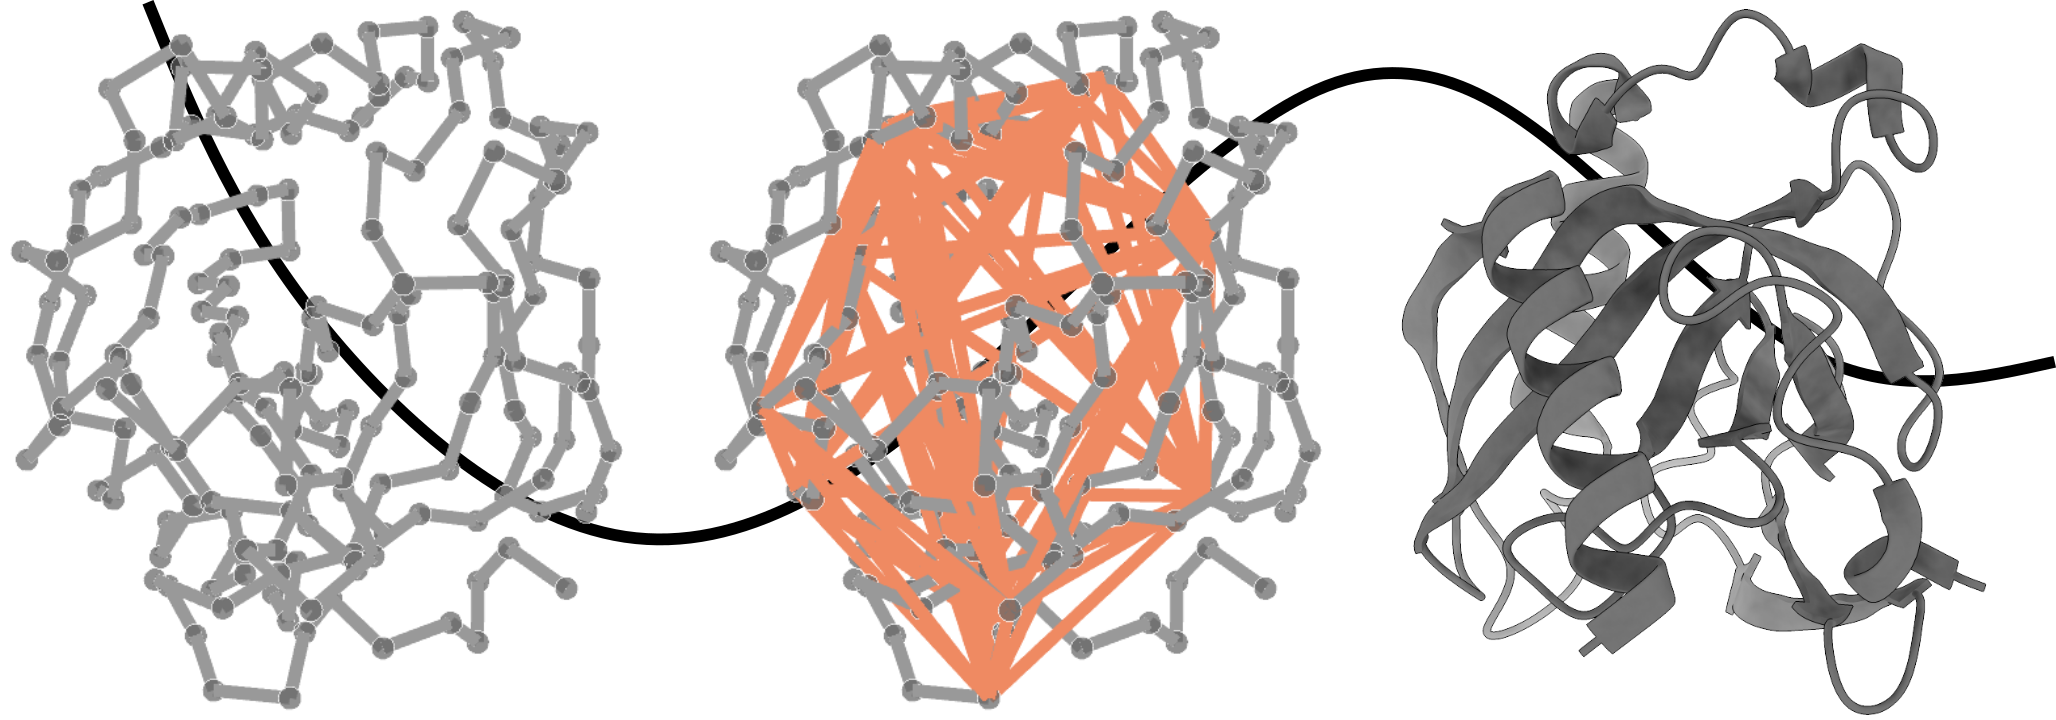
\includegraphics[width=0.6\textwidth]{Chapter.1/Figures/chapter1_cover.png}
    \end{center}
}
%
\begin{flushleft}
    \vspace*{\fill}
    \rule{\textwidth}{1pt}\\[0cm]
    This chapter includes parts of the following publication:\\
    \textbf{Complexome profiling - exploring mitochondrial protein complexes in health and disease}\\
    \footnotesize
    \vspace{0.3cm}
    Alfredo Cabrera-Orefice, Alisa Potter, Felix Evers, Johannes F. Hevler and Sergio Guerrero-Castillo \\
    %\vspace{0.3cm}
    \textbf{\emph{Front Cell Dev Biol.}} (2022), 9:796128, doi: 10.3389/fcell.2021.796128. \emph{Review}\\
\end{flushleft}
\newpage
%
\section{Prelude - The importance of probing protein interactions}
\lettrine[lraise=0.1, nindent=0em, slope=-.5em]{P}{roteins}, the so-called “workhorses” of life, are the tools that make living machines work  \cite{Adams_2008}. The vast majority of biological processes are thus structured, mediated and executed by these macromolecules. Even though many single proteins do perform specific functions by their own, most proteins habitually interact with other proteins, DNA, RNA and lipid molecules rather than acting individually for achieving their biological tasks. The resultant protein complexes can form transient or steady interactions, which also correlate with the type of biological processes they are involved in \cite{De_Las_Rivas_2010}. For example, housekeeping cell processes are likely performed by a large fraction of physically stable protein complexes, whereas in signaling, cell migration, membrane trafficking, metabolic response and other highly dynamic processes, involvement of transient complexes is required for rapid responses and adaptation. The entire set of multi-protein complexes in a cell or compartment is referred to as the complexome \cite{Ceulemans_2006, Deshaies_2002, Lasserre_2006}.

In situations where impaired interaction of the elements of a protein complex affects its proper formation; e.g., due to genetic mutations, the related cell process(es) could be compromised and result in biological dysfunction. Higher complexity in multicellular organisms is of course accompanied by larger complexomes than those from unicellular species. Therefore, alterations in protein complexes may affect not only multiple cell processes, but also lead to severe pathophysiological issues at the tissue/organ level. An integral elucidation of both complexomes and protein interaction networks; i.e., interactome \cite{Vidal_2011} under different cellular scenarios, becomes crucial to fully comprehend the molecular mechanisms behind cell physiology and disease.

Numerous biochemical, biophysical, structural, genetic, microscopy and mass spectrometry (MS) approaches have been applied to characterize protein complexes. Although these methods have different principles, in most cases, they require experimental interventions, cell/tissue fractionation, protein extraction and/or time-consuming protocols prior to data collection and analyses. Besides, the amount of information obtained is often limited to one or a small set of protein complexes. The recent breakthrough in quantitative high-throughput technologies and bioinformatic tools has substantially increased the efficiency and quality of the large-scale identification of protein interactors \cite{Iacobucci_2021, Low_2021}. Accordingly, an outstanding volume of evidence on the composition, 3D structure, interactions and molecular roles of hundreds of protein complexes is now easily accessible through multiple repositories, such as RCSB PDB \cite{Burley_2021}, STRING \cite{Szklarczyk_2021}, CORUM \cite{Giurgiu_2019}, BioGRID \cite{Oughtred_2021}, Pfam \cite{Mistry_2021}, Complex Portal \cite{Meldal_2021}, NCBI \cite{Coordinators_2016} and UniProt \cite{UniProt_2021}. Yet, a substantial fraction of the protein interactors reported in those databases still lack full validation of their occurrence \emph{in vivo} by using novel and more reliable methods.

Further, function and capability to interact is closely linked to a proteins three-dim\-ensional conformation. As such, interrogating structures and interactions of proteins is key to understand cellular processes and therefore has evolved into a significant area of biological research \cite{De_Las_Rivas_2010, Russell_2004}. Discerning structural details of proteins and macromolecular complexes is performed using techniques such as X-ray crystallography, nuclear magnetic resonance (NMR), Small Angle X-ray Scattering (SAXS), cryo-transmission electron microscopy (cryo-EM) as well as cryo-electron tomography (cryo-ET) \cite{Cerofolini_2019, Dunstone_2017}. Especially, X-ray crystallography, NMR and cryo-EM with the ability of providing atomic structures of proteins and protein complexes contributed unprecedented structural and biological insights into processes crucial for cellular life \cite{Cate_1999, Englmeier_2019, O'Connell_2009}. Despite these accomplishments, these more standard techniques also have their limitations. Foremost, they predominantly require a highly purified sample for analysis, consequently proteins and protein complexes are rarely studied in their naïve cellular environment. In recent years it has become very apparent that structures need to be solved \emph{in situ} to fully understand biological processes, but methods enabling \emph{in situ} structural characterization lagged behind \cite{Lucic_2008}. New developments an opposing the reductionist approach, cryo-ET allows to image whole organisms, tissues, cells and organelles. Recorded images are subsequently reconstructed into three-dimensional tomograms, enabling the investigation of macromolecular complexes in a near native environment \cite{Doerr_2017}. Although cryo-ET holds a future potential to image the entire proteome of a cell, it is currently still limited to highly abundant, very large protein complexes such as ribosomes or respiratory chain assemblies \cite{Davies_2014, Turk_2020}. Alternatively, mass spectrometry (MS) allows to study macromolecules and their assemblies independent of their size and abundance and has thereby evolved into a new pillar in the structural characterization of the proteome (structural proteomics). Since the development of electrospray ionization (ESI) \cite{Fenn_1989, Yamashita_1984} and matrix-assisted laser desorption ionization (MALDI) \cite{Karas_1988} in the mid 1980's, rapid technical advancements resulted in a diverse suit of MS-based techniques for the structural characterization of proteins and protein assemblies. A selection of popular structural MS methods is depicted in \textbf{\autoref{fig:fig1}}. The diversity of available methods not only arose from the many different macromolecules present in the proteome but also from different analysis strategies. Fundamentally, MS-based approaches can be divided into protein-centric and peptide-centric strategies \cite{Soldi_2013}. While protein-centric strategies enable the characterization of intact proteins and protein complexes, peptide-centric approaches delineate structural information by enzymatically digesting proteins into peptides prior to MS analysis. Despite those differences, MS based methods can provide highly complementary structural information on proteins and protein complexes such as their conformation, post-translational modifications (PTMs), surface properties, interaction interfaces, stoichiometry and subunit connectivity. Especially in combination with computational modeling, MS based technologies provide a toolbox that is helpful to unravel structural details that would not be easily accessible with other structural approaches.

\begin{figure*}[hbt]
    \center
    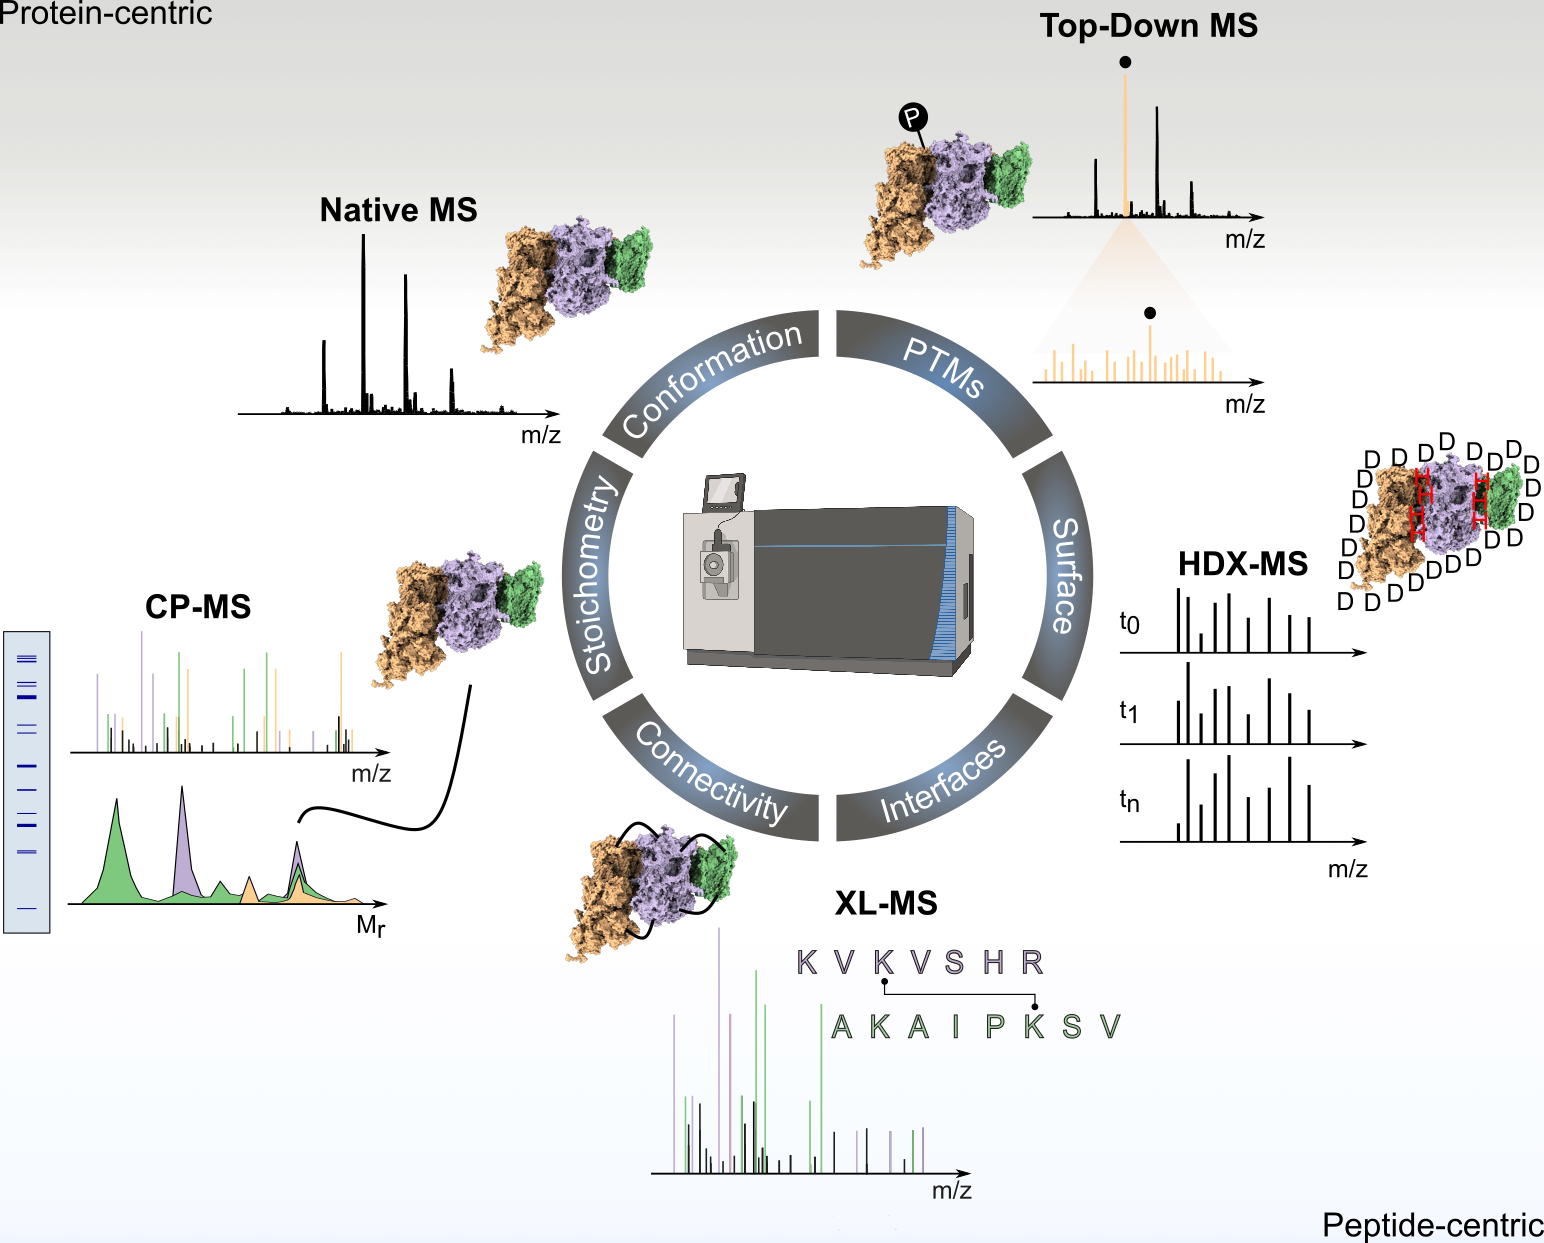
\includegraphics[]{Chapter.1/Figures/Figure1.png}
    \caption{\textbf{Overview of various types of structural MS techniques that can be applied for the characterization of proteins and protein complexes.} The top panel describes protein-centric approaches (native-MS, top-down MS), where intact proteins are analyzed. Complementary, peptide-centric methods (XL-MS, CP-MS, HDX-MS) depicted in the bottom panel, delineate structural information of proteins and protein complexes from peptides.}
    \label{fig:fig1}
\end{figure*} \clearpage
Amongst the versatile MS based toolbox, cross-linking mass-spectrometry (XL-MS) and complexome profiling mass-spectrometry (CP-MS) have emerged as powerful methods to structurally and functionally characterize proteins and protein-protein interactions \cite{Steigenberger_2020}. Nonetheless, both methods also present drawbacks that significantly hamper an adequate structural characterization of protein assemblies. In this thesis I present a collection of XL-MS based advancements that significantly improve the structural and functional analysis of protein complexes in mitochondria. In short, chapter 2 and 3 introduce XL-MS and CP-MS as highly complementary methods, allowing the detailed characterization of protein complexes. Chapter 4 and 5 highlight how XL-MS can aid the identification and characterization of protein complexes using cryo-ET as well as computational structure prediction methods. In the subsequent parts of this introduction, I will succinctly review the fundamentals of XL-MS and CP-MS. The last part will be devoted to how XL-MS in combination with CP-MS and computational modeling, whereby I describe how such a combination can benefit our molecular understanding of mitochondrial protein complexes.
%
\section{The fundamentals of probing protein structure and interactions with XL-MS}
Chemical cross-linking is a special category of protein chemical modifications, and as such it was developed already over 70 years ago to elucidate the chemical and biological function of proteins \cite{French_1945}. Using a cross-linking reagent non-covalent interactions within or between amino acid side-chains of proteins are converted into covalent chemical bonds, stabilizing proteins or protein complexes so that they can be analyzed using methods that normally could denature proteins \cite{Means_1998, Naowarojna_2021}. Like that, cross-linking paired with gel electrophoresis enabled the identification of protein-protein interactions in ribosomes of \emph{Escherichia coli} as early as in the 1970s \cite{Clegg_1974, Sun_1974}. The development of peptide-centric MS methods roughly 30 years later substantially increased the impact of cross-linking for the structural characterization of proteins and respective complexes \cite{Rappsilber_2011, Rappsilber_2000}. Combining cross-linking and peptide-centric MS (XL-MS) enabled not only the fast and sensitive identification of cross-linked proteins but furthermore promised to reveal the position of interacting residues, thereby catering valuable restraints for the structural characterization of proteins and protein complexes. Advances in instrumentation, bioinformatics tools as well as the development of innovative-, MS compatible cross-linkers further increased the application of XL-MS, for instance to study also protein-nucleic acid interactions \cite{Gotze_2021, Wong_1991}.
%
\subsection*{An overview of available cross-linking reagents}
To date, a variety of MS compatible cross-link reagents have been introduced, all aiming at efficiently leveraging spatial distance restraints representative of the in-solution state of proteins and protein complexes. To accomplish this, most of the available reagents typically share a similar structural design, in which two reactive moieties (most commonly amine-reactive) are connected by a spacer arm. However, to account for different applications, e.g. different type of samples as well as to ease the identification cross-linked peptides more elaborated designs have been developed \cite{Steigenberger_2020}. To counteract the low efficiency of the cross-linking reaction, and the subsequent low abundance of cross-linked peptides \cite{Leitner_2014, Leitner_2010}, cross-linkers containing enrichable moieties have been introduced. The usage of linkers with enrichable handles like biotin, phosphonic acid as well as azides proved to significantly increase the number of detected cross-linked peptides, by reducing the huge background of non-modified peptides \cite{Matzinger_2020, Steigenberger_2019, Tan_2016}. Additionally, to simplify the computational challenges that are accompanied with identifying cross-linked peptides, so-called “cleavable” cross-linkers have been introduced. Cleavable-cross-linkers possess a labile moiety between the two reactive groups, which can be cleaved during MS analysis. This reduces the subsequent MS2 sequencing to just a single precursor mass originating from an individual peptide with respective part of the cross-linker attached. In contrast, “non-cleavable” cross-linkers stay intact during MS analysis for which subsequent spectra contain fragment ions of the two linked peptides which significantly hampers the identification \cite{Kao_2011}. A more detailed explanation of MS identification of cleavable and non-cleavable cross-linked peptides will follow below.

\begin{figure*}[hbt]
    \center
    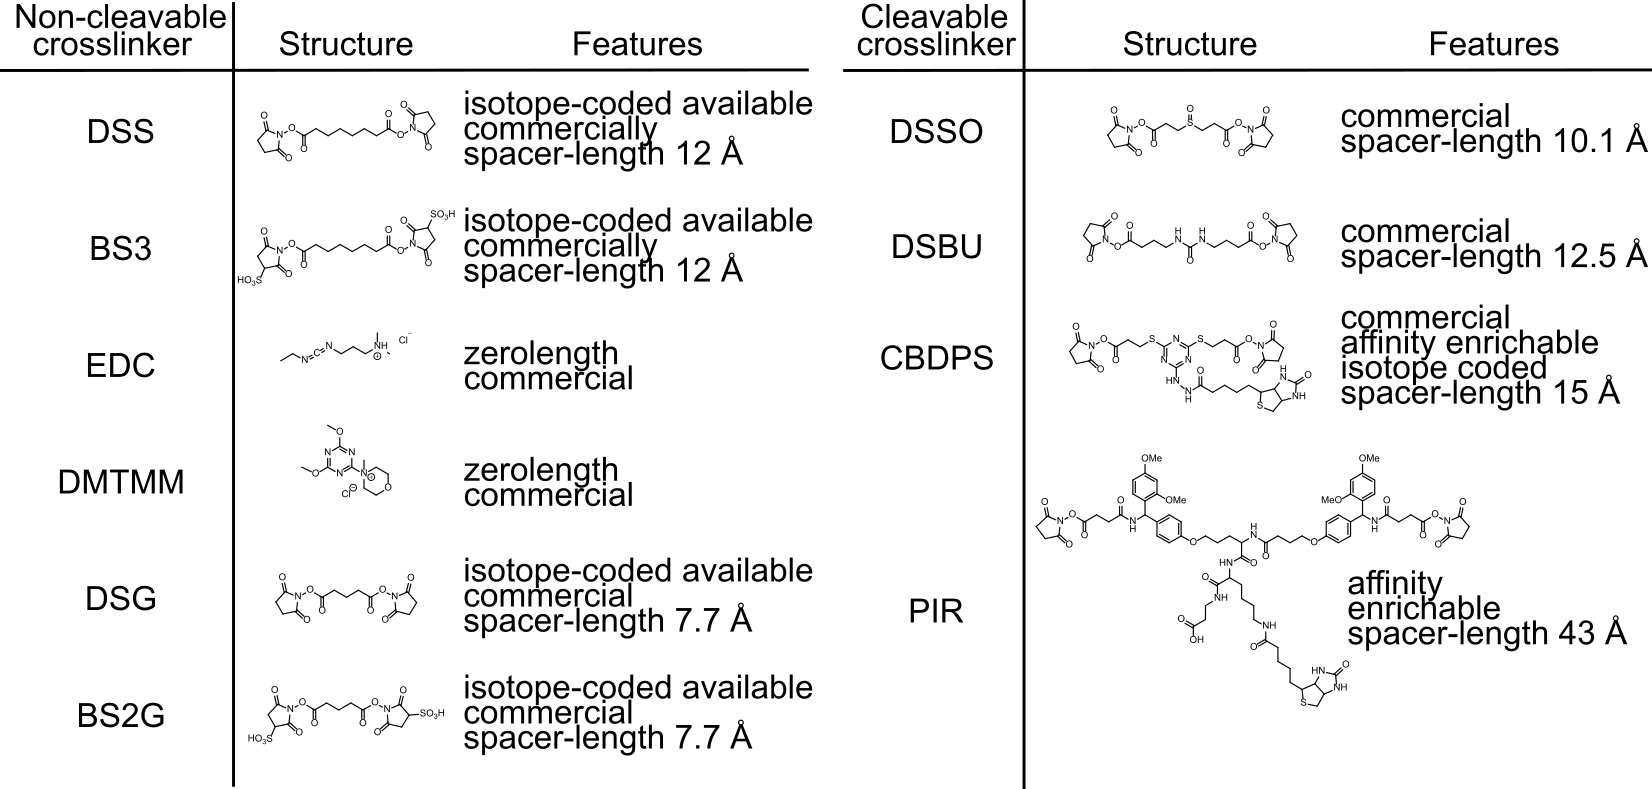
\includegraphics[]{Chapter.1/Figures/Figure2.png}
    \caption{\textbf{Overview of MS-compatible cross-linking reagents.} Figure adapted with permission from \cite{Steigenberger_2020}}
    \label{fig:fig2}
\end{figure*}
Lastly, to further increase the stringency for produced distance restraints, so called “zero-length” cross-linkers have been introduced. These compounds mediate the direct conjunction of two proximal residues with no intervening spacer arm or linker. This theoretically reduces the produced distance restraints to only the length of the side chains ($\sim$15 Å), as opposed to cross-linkers with a spacer arm that produce distance restraints >25 Å. Limiting possible residue-residue distances is especially beneficial when utilized as constraints in computational modelling of proteins or protein complexes, as it reduces the number of possible orientations \cite{Leitner_2014}. An overview of some of the more commonly used cross-linkers is depicted in \textbf{\autoref{fig:fig2}}.
%
\subsection*{XL-MS to characterize protein-protein interactions in mitochondria}
Most cross-linking studies are performed on purified proteins and protein complexes, however in recent years an increasing amount of applications have been reported for more complex systems like whole organelles, cells and even tissue as reviewed in for instance \cite{O'Reilly_2018}. An advantage of working with purified proteins and protein complexes is the significantly simplified detection and identification of cross-links using MS including a more straightforward data analysis. Notwithstanding the challenge, only XL-MS studies of naive systems such as intact mitochondria, can provide a comprehensive interaction network thereby enabling a better understanding of biological processes and dependencies. To tackle the complexity of such systems, several technical and experimental advancements have been presented over the past years enabling the successful identification of mitochondrial protein interactions using XL-MS \cite{Liu_2018, Ryl_2020, Schweppe_2017}.  Given the complexity of mitochondrial proteomes, the selection of a suitable cross-linker, prior to MS-analysis is essential (\textbf{\autoref{fig:fig3}A}). Gas-phase cleavable cross-linkers such as DSSO \cite{Kao_2011} or cross-linkers with an enrichment handle such as PhoX \cite{Steigenberger_2019} significantly simplify the subsequent identification of the XLs. Although NHS- reactive cross-linkers, covalently linking proximal lysine-side chains, are still most commonly applied in cross-linking experiments \cite{Steigenberger_2020}, cross-linkers with an alternative side-chain reactivity are valuable reagents to increase the cross-link coverage. The zero-length cross-linker DMTMM, which promotes the condensation between carboxyl-groups (Glutamic acid, Aspartic acid) and primary amines (Lysines) can increase the cross-linking coverage of membrane proteins, as hydrophobic patches which typically carry none or very few Lysine residues could be targeted via Glutamic acid and Aspartic acid residues \cite{Hevler_2021b}. Importantly, before each application, cross-linking conditions, e.g. the ratio of cross-linker to protein or choosing of a suitable cross-linking buffer, need to be carefully optimized \cite{O'Reilly_2018}. After cross-linking, mitochondria are disrupted either mechanically (e.g. sonication) or by using detergents (e.g. Triton-X-100) and soluble proteins are subsequently denatured, reduced, and alkylated, alike in standard bottom-up proteomics experiments. Before enzymatic digestion of soluble proteins into peptides, contaminations such as lipids and detergents are removed by precipitation or phase extraction \cite{Klykov_2018}. After digestion, cross-linked peptides, which can either stem from the same protein (intra cross-link) or from two distinct proteins (inter cross-link), are significantly less abundant than their “linear” (non cross-linked) and “mono-linked” counterparts \cite{Leitner_2014, Leitner_2010, Sinnott_2020} (\textbf{\autoref{fig:fig3}B}). Mono-linked peptides are linear peptides which carry the cross-linker that is quenched or hydrolyzed on the other reactive group rather than attached to another peptide. In contrast to linear peptides, mono-linked peptides contain structural information and are commonly used to assess protein surface accessibility as well as to support scoring of structural models \cite{Sinnott_2020}. The sub-stoichiometric reaction efficiencies render the identification of cross-linked peptides challenging, especially in complex samples such as intact cell and mitochondria. To obtain satisfactory identification of cross-linked peptides relative to their linear counter parts, an enrichment step is often essential (\textbf{\autoref{fig:fig3}C}). Enrichment most often takes place via chromatographic methods, such as strong-cation-exchange (SCX) fractionation, that can be used to separate doubly charged linear (tryptic) peptides (carrying a charge at the N and C terminus) from higher charged, cross-linked peptides (typically carrying double the number of charges). In case an enrichment handle such as a phosphonate group (PhoX) is used, cross-linked peptides can be captured onto a suitable material (e.g. Fe3+ IMAC), thereby allowing the separation from linear peptides. After enrichment, cross-linked peptides are identified following different MS acquisition strategies (\textbf{\autoref{fig:fig3}D}). Which MS acquisition method to use, is largely determined by the applied cross-linker \cite{Liu_2017a}. Lastly, recorded XL-MS spectra can be searched using various software suits
\begin{figure*}[p]
    \center
    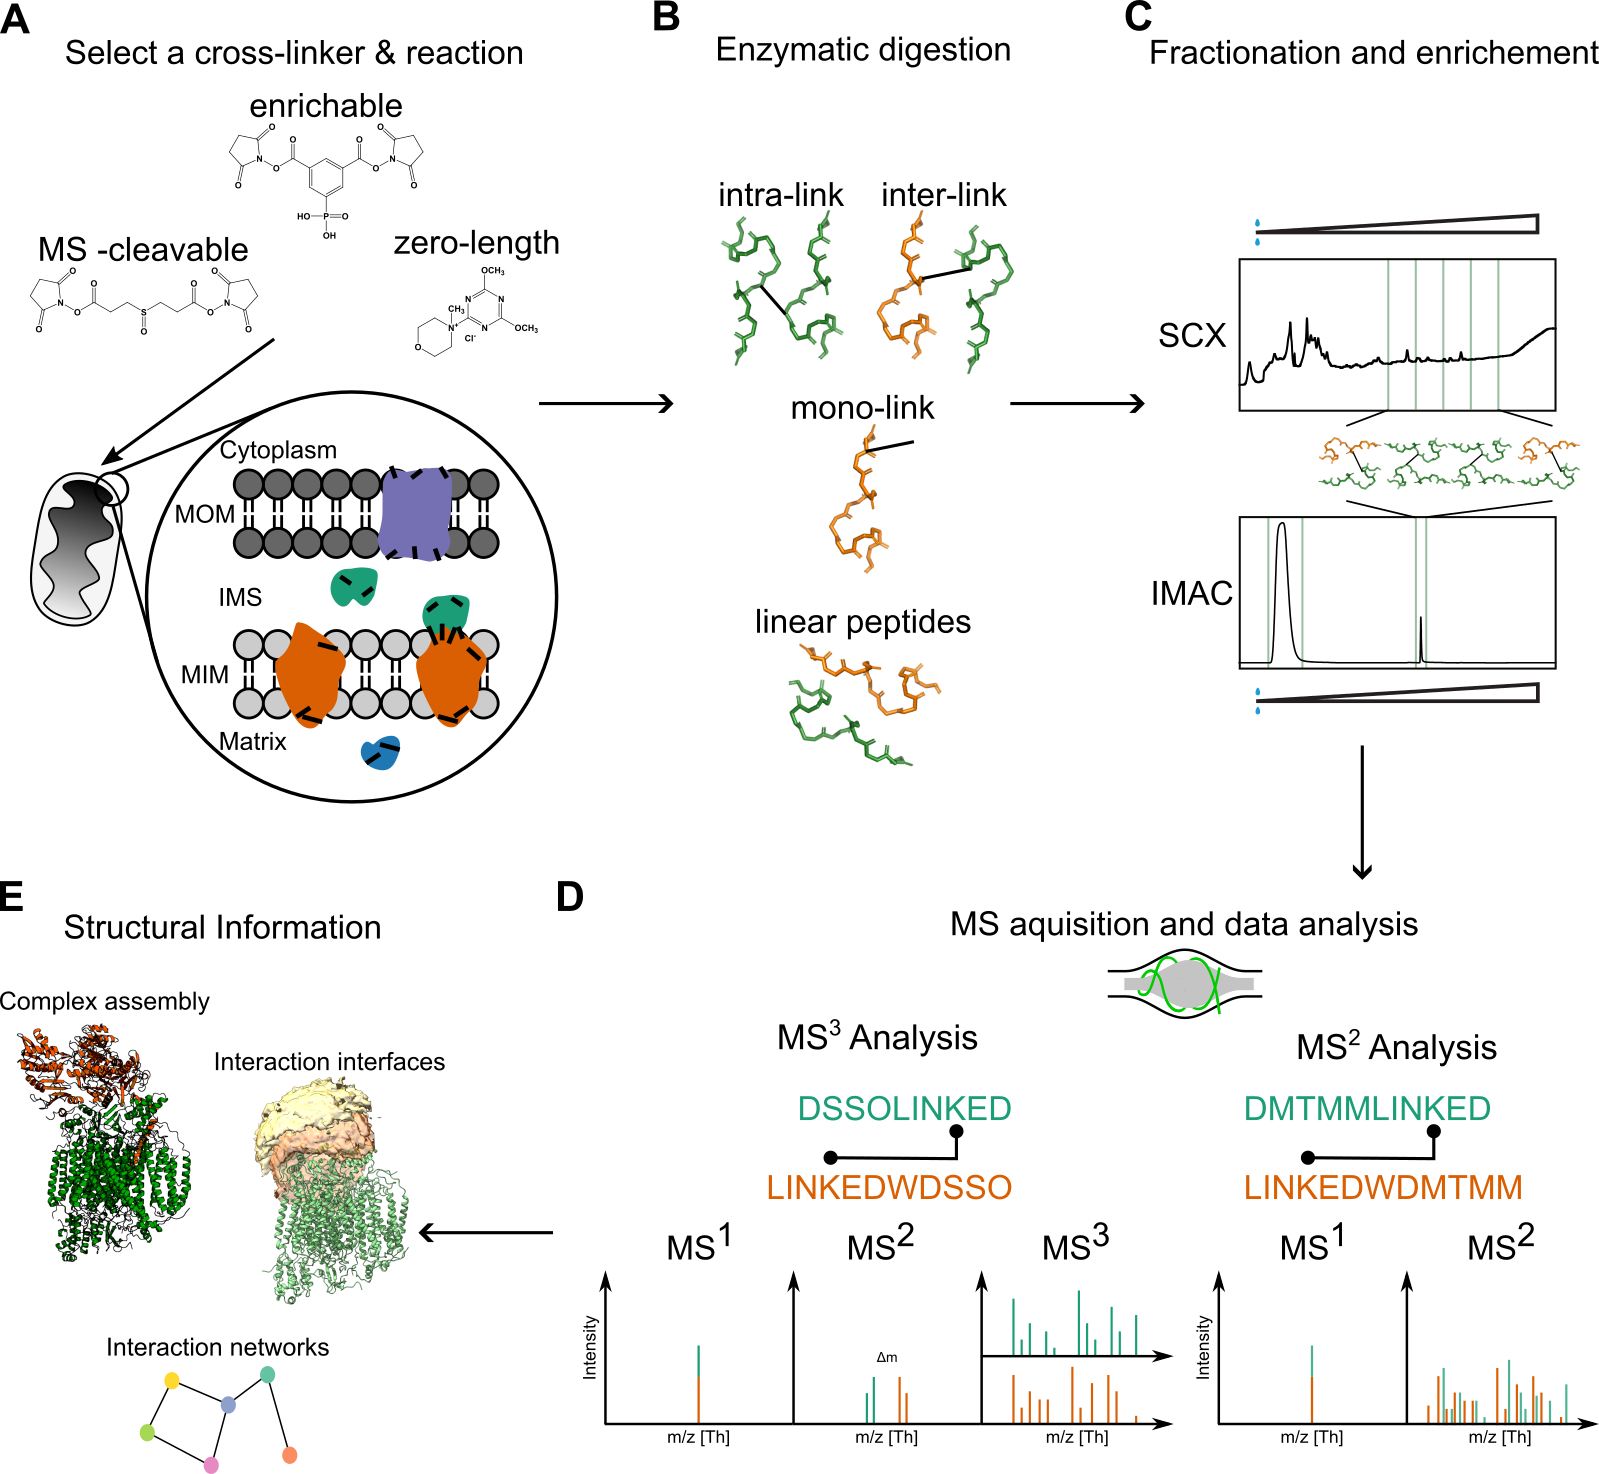
\includegraphics[width=0.95 \textwidth]{Chapter.1/Figures/Figure3.png}
    \caption{\textbf{Experimental strategies for the analysis of proteome-wide protein-protein interactions in mitochondria.} \textbf{A.} Cross-link reagents comprise various chemistries as highlighted in \textbf{\autoref{fig:fig2}}. For cross-linking mitochondria, reagents with a cleavable spacer arm, enrichable handle or an alternative amino-acid reactivity are beneficial to increase the number of cross-link identifications. DSSO is depicted here as an example for a cleavable cross-linker. PhoX is depicted as an example for a cross-linker with an enrichment handle (phosphonic acid) and DMTMM is depicted as example for a zero-length cross-linker. For each application, conditions such as concentration and reaction time need to be carefully optimized to achieve optimal cross-linking. \textbf{B.} After solubilization of mitochondrial membranes proteins are enzymatically digested, producing a mixture of cross-linked and linear peptides. Cross-links can be formed within protein sidechains (intra link) and between sidechains of different proteins (inter link). Additionally, linear peptides with the cross-linker attached (mono-links) can be formed. \textbf{C.} To increase MS identification, cross-linked peptides are separated from linear peptides using chromatographic methods, such as strong-cation-exchange chromatography (SCX) or Fe3+ IMAC enrichment chromatography. \textbf{D.} Depending on the chosen cross-linker (e.g. gas-phase cleavable or non-cleavable) different MS acquisition strategies can be applied, to increase the likelihood of identifying a cross-linked peptide. \textbf{E.} Different software solutions as described in the text can be utilized to identify linked peptides. Information of cross-linked experiments can be used to elucidate protein-protein networks, interaction interfaces as well as to structurally model protein complex assemblies as described in the text. Figure adapted from \cite{Hevler_2021b}.}
    \label{fig:fig3}
\end{figure*}
such as pLink2 \cite{Chen_2019b}, MeroX \cite{Gotze_2015}, StavroX \cite{Gotze_2012}, Xi \cite{Chen_2019a}, Kojak \cite{Hoopmann_2015} and XlinkX \cite{Klykov_2018}. However, not all software solutions are capable of analyzing all MS-acquisition strategies or cross-link reagents (e.g. MS3, DSSO), as such software capability as well as availability should be taken into consideration when designing a XL-MS experiment. Likewise, methods for FDR calculations might differ across platforms, thereby impacting the quality and ambiguity of outputted XL-MS results \cite{Matzinger_2022}. Careful manual validation of identified cross-linked peptides is still advisable before utilizing them for the structural characterization of protein complexes (\textbf{\autoref{fig:fig3}E}). Strategies for MS-acquisition, and applications of XL-MS for structural characterization of proteins and protein complexes will be further discussed in the following sections.
%
\subsection*{XL-MS-data acquisition}
In classical bottom-up proteomics, linear peptides are identified based on their accurate mass (measured at the MS1 level) and sequence specific fragment ions (measured at the MS2 level). To be analyzed within the mass spectrometer, peptides are first ionized and thereby separated from their carrier medium (usually aqueous or organic phase). Charged and ionized peptides are next transmitted into the mass spectrometer, where the mass of the intact peptide-ion is determined by a mass analyzer (MS1 signal). The mass of each ion is measured by monitoring their motion through the mass analyzer, which is dependent on the mass to charge ratio (m/z). Work presented in this thesis utilized instruments equipped with quadrupoles, linear ion traps (LIT) as well as an Orbitraps as mass analyzers. To confidently determine the correct peptide sequence, the peptide ion is fragmented inside the mass spectrometer providing additionally m/z values for its fragment ions (MS2 level). Depending on the fragmentation technique used, different fragment ions corresponding to cleavage of the peptide backbone can be observed. Most frequently, collision-induced dissociation (CID) \cite{Hunt_1986} and higher-energy C-trap dissociation (HCD) \cite{Olsen_2007} fragmentation techniques are applied, producing b and y fragment ions that reflect N- and C-terminal fragments, respectively being cleaved at the peptide bonds. For XL-MS applications, further fragmentation of an isolated fragment ion (MS3 level) can be very useful, however not all mass spectrometers are capable of performing such higher order, e.g. MS3, experiments \cite{Liu_2017a, Lossl_2016}.\\
For XL-MS experiments, the seemingly well-established MS analysis for the identification of linear tryptic peptides is substantially impaired, due to the fact that the cross-linked peptide is composed of two covalently bound linear peptides. As such, the two peptide moieties presents in these cross-linked peptide precursor ions are normally co-fragmented in the same MS2 spectra, often with different fragmentation efficiencies for the two peptide moieties hampering the full identification of both \cite{Liu_2017a}. To circumvent impaired fragmentation and to increase the fragmentation efficiency, cross-linked peptides are commonly fragmented using multiple collision energies (CID/HCD), resulting in more informative fragmentation spectra (MS2 method). Importantly, also the cross-link reagent moiety can impact the fragmentation. Consequently, collision energies need to be optimized for each cross-linker to obtain the best fragmentation efficiency. Likewise, combining complementary dissociation methods such as CID/HCD and electron transfer dissociation (ETD) can be applied for an improved fragmentation (MS2-MS2 method) \cite{Campbell_2009, Frese_2012, Liu_2017b} (see \textbf{\autoref{fig:fig3}D}). Additionally, gas-phase cleavable cross-linkers \cite{Sinz_2017}, such as DSSO have been developed to address such impaired fragmentation. Such cross-linkers are cleaved during the fragmentation process of the XL peptide ions inside the vacuum of the mass analyzer, thereby enabling the dissociation of the cross-linked peptides and greatly improving fragmentation and thus cross-link identification of the two peptide moieties \cite{Liu_2017a}. When measuring on mass spectrometers capable of MS3 analysis, a dual-fragmentation strategy for cleavable cross-linkers can be applied. In such an approach, a survey scan (MS2) is performed, in which a dissociation energy is chosen that specifically breaks the cleavable cross-linker thereby giving rise to signature ions with a unique mass difference corresponding to the cleaved cross-linked peptide each with a part of the cross-link moiety attached. Whenever the mass spectrometer identifies the XL-peptide signature ions, a subsequent isolation and fragmentation step is performed to obtain better sequence information (MS3 analysis) \cite{Liu_2017a, Sinz_2017} (see \textbf{\autoref{fig:fig3}D}). The utilization of gas-phase cleavable cross-linkers in combination with MS3 acquisition strategy has been found to be extremely useful for the analysis of proteome-wide XL-MS experiments such as cell lysates \cite{Klykov_2018, Liu_2017a} as well as intact organelles such as mitochondria \cite{Liu_2018} or nuclei \cite{Fasci_2018}. Notwithstanding, it was recently shown that MS2- and MS2-MS2 acquisition methods can outperform MS3 acquisition strategies in terms of unique crosslink numbers \cite{Matzinger_2022}, suggesting that the new generation of MS2 capable mass-spectrometers can also be used for analysis of proteome-wide, gas-phase cleavable XL-MS experiments.
%
\subsection*{Applications of XL-MS for the structural characterization of protein complexes}
Beyond what is well possible using more common techniques in structural biology, XL-MS can also be performed under naïve cellular conditions, reducing possible artifacts that may occur during recombinant expression and/or purification of proteins and protein complexes \cite{Niedzialkowska_2016}. In the latter case additional artefacts may occur during in vitro reconstitution of a protein complex. Additionally, benefits of probing protein-protein interactions \emph{in vivo} have been shown in work on mouse heart mitochondria, for which a number of protein-protein interactions could only be observed in intact mitochondria and not upon membrane disruption \cite{Liu_2018}. XL-MS studies applied to cell lysates or intact organelles such as mitochondria, have successfully captured proteome-wide PPIs, thereby enhancing our understanding of how the proteome is wired \cite{Fasci_2018, Klykov_2018, Liu_2017b, Ryl_2020, Schweppe_2017} (\textbf{\autoref{fig:fig4}A}). While such interaction networks are also commonly generated through other MS based methods such as affinity-purification MS (AP-MS) \cite{Huttlin_2017, Krogan_2006}, intra and inter cross-links generated by XL-MS additionally provide information that can be used for the structural characterization of proteins and protein complexes \cite{Bullock_2018, Klykov_2018, Orban-Nemeth_2018}. Intra protein cross-links provide information about proximal amino acids within a protein, which can be applied as distance restraints in subsequent computational modeling \cite{Orban-Nemeth_2018} (\textbf{\autoref{fig:fig4}B}). Distances for cross-link restraints applied in computational modeling are mostly calculated between C\(\alpha\)-C\(\alpha\), by summing the length of each side chain and the length of the cross-linker. As side-chains and cross-linkers are highly flexible, distance restraints are typically provided as a range (with a minimum and maximum value) rather than a defined distance value. Modeling software`s such as I-Tasser \cite{Yang_2015}, Robetta \cite{Kim_2004} and Modeller \cite{Webb_2016} employ set cross-link constraints for model building as well as for scoring features (e.g. geometry) of the structure which may not be evaluated by standardly used score terms. Recent breakthroughs in the field of protein structure prediction by AI driven tools such as AlphaFold2 \cite{Jumper_2021} and RoseTTA-fold \cite{Baek_2021}, enable the generation of structural models based solely on the amino acids sequence of a protein. However, validation and finding the biological relevant confirmation can be time consuming and challenging with only having the provided output scores at hand. For this, it was recently shown that intra cross-links can be utilized to aid the validation process as well as to pinpoint towards biologically active structural conformations \cite{McCafferty_2022}.

Moreover, \emph{ab initio} protein-protein docking offers a possibility to computationally predict protein complexes and protein-protein interfaces, given that the structures of the individual sub-units are known \cite{Dominguez_2003, Vakser_2014}. For most of the available programs complex
conformations are predicted by rotating and translating one complex component (often the smaller protein) around the other one, which is fixed in space.

\begin{figure*}[htb]
    \center
    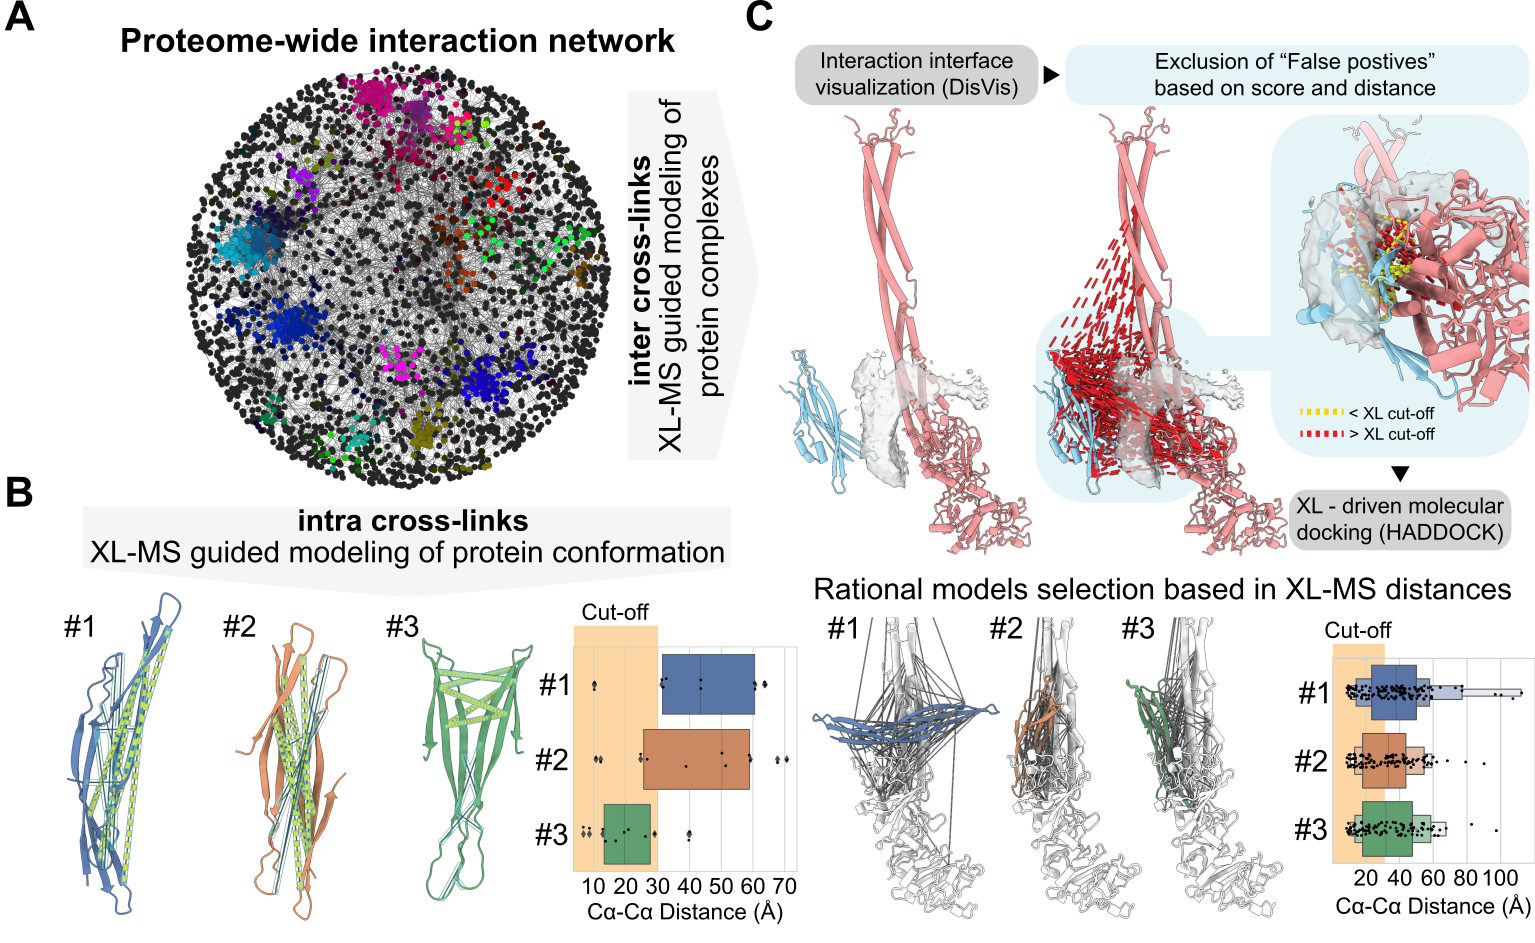
\includegraphics[]{Chapter.1/Figures/Figure4.png}
    \caption{\textbf{Applications of XL-MS for the structural characterization of proteins and protein complexes} \textbf{A.} When XL-MS is applied on high complex samples, such as cell lysates or intact organelles, protein-protein interaction networks can be generated. Protein interaction networks highlight how a soluble proteome is wired. Proteins are shown as black nodes, with proteins that have a similar GO functional annotations \cite{Ashburner_2000} being depicted in bright colors. \textbf{B.} Intra protein cross-links can be utilized to guide structural modeling of a protein conformations, as well as to validate AI derived structural models. \textbf{C.} Inter protein cross-links can be utilized to model protein complexes observed in the interaction network. Information about proximal amino acids is validated and utilized to identify interaction interfaces and active interface residues (e.g. using DisVis \cite{van_Zundert_2015}). True positive inter-crosslinks as well as information about active interface residues can subsequently be used as input for protein-protein docking (e.g. using Haddock \cite{van_Zundert_2016}). Validation of generated complex models can be performed by mapping obtained inter cross-links onto final structures. Figure adapted from \cite{Lagerwaard_2022} with permission. Data to generate the protein-protein interaction network was obtained from \cite{Costanzo_2016}}
    \label{fig:fig4}
\end{figure*}\clearpage
This approach, however, is still very time consuming and computationally expensive as all theoretically possible conformational spaces have to be sampled and scored \cite{Dominguez_2003, van_Zundert_2016}. Inter protein cross-links identified in XL-MS experiments, provide information about the arrangement of proteins within a complex. Utilizing inter cross-links as additional restraints to guide the docking process alongside traditional energetics and shape complementarity can therefore significantly reduce the possible conformational space and increase the chance for the prediction to result in a unique solution \cite{Dominguez_2003, van_Zundert_2016} (\textbf{\autoref{fig:fig4}C}). HADDOCK \cite{Dominguez_2003, Orban-Nemeth_2018} (High Ambiguity Driven protein-protein Docking) is a powerful tool that can make use of biochemical and/or biophysical interaction data such as inter cross-links observed in XL-MS experiments. To utilize cross-links for guiding structural docking, the provided information content needs to be first evaluated. DisVis \cite{van_Zundert_2015} is a software suit enabling the identification of false-positive cross-links as well as the characterization of surface residues that are most often contacted in all possible models (interface residues). True-positive cross-links together with active interface residues are employed as additional restraints to predict a protein complex and later for validation and model selection. Besides guiding protein-protein docking, cross-linking data was shown to benefit other structural and modeling techniques, for instance with the assignment of ambiguous densities in cryo-EM maps \cite{Herzog_2012, Kyrilis_2021b} or with identifying and refining high confidence models predicted for protein complexes based on AI \cite{Burke_2021}.

Although the prime technology used for the work described in this thesis is cross-linking mass spectrometry, several of the chapters involved the use of another powerful approach, namely complexome profiling. Below I describe succinctly also this approach, largely adapted from \cite{Cabrera-Orefice_2022}, and include a description of some of the more recent applications of this method especially looking into mitochondrial protein complexes in all the kingdoms of life.
%
\section{The fundamentals of characterizing protein complexes with complexome profiling mass spectrometry (CP-MS)} \label{sec:CP_MS_intro}
The first requisite to carry out a complexome profiling (CP) experiment is the collection of biological material; e.g. tissue pieces/biopsies, cultured cells, enriched cell fractions, purified organelles, etc. These materials might also come from previous experimental interventions. Homogenization and cell fractionation methods should aim to keep the native state of protein complexes. For solubilization of membrane proteins, it is recommended to use mild, non-ionic detergents; e.g., Triton X-100, NP-40, dodecyl-maltoside, octyl-glucoside or digitonin \cite{Eubel_2005, Wittig_2006}. Next, native protein extracts are separated by a so-called “untargeted” method \cite{Iacobucci_2021}, such as native electrophoresis, size-exclusion chromatography or density gradient ultracentrifugation (\textbf{\autoref{fig:fig5}}). Regardless of the type of protein separation, CP follows a well-defined protocol that slightly differs among variants. In all cases, protein complexes are separated by size, hence, by shape and molecular mass. Each fraction is further digested with high-purity and specific proteases (e.g., trypsin, chymotrypsin and endoproteinase Lys-C) followed by MS/MS identification of the resulting peptides \textbf{\autoref{fig:fig5}}; i.e., bottom-up proteomics strategy \cite{Zhang_2013}.\\
Prior to MS analysis, peptides are usually separated based on their hydrophobicity by reversed-phase high-performance liquid chromatography (RP-HPLC) followed by electrospray ionization (ESI) to produce gas phase ions \cite{Zhang_2013}. The majority of MS data for CP studies has been acquired in data-dependent mode (DDA); i.e. collection of a predefined number of precursor ions for fragmentation during the MS2 cycle is done according to their charge states and abundance \cite{Hu_2016}. In conventional DDA modes, the possibility to identify low abundant peptides thus becomes significantly limited. To avoid this issue, acquisition strategies in data-independent mode (DIA) \cite{Krasny_2021}, such as sequential window acquisition of all theoretical mass spectra (SWATH-MS) \cite{Gillet_2012}, in which fragmentation of all precursor ions identified in the MS1 cycle can be analyzed in the MS2 cycle, have recently been introduced to CP-like workflows \cite{Bludau_2020, Calvo_2020, Heusel_2019}.

MS spectra are routinely matched against a proteome database of the species of interest by using a variety of software/search engines (\textbf{\autoref{fig:fig5}}), such as Mascot \cite{Perkins_1999}, openMS \cite{Rost_2016}, PEAKS DB \cite{Zhang_2012}, Proteome discoverer \cite{Orsburn_2021}, Protein Prospector \cite{Chalkley_2005} and MaxQuant \cite{Tyanova_2016a}. In case that the proteome of the studied organism is not yet available or fully annotated, metagenome or transcriptome data are useful to generate a list of proteins and perform the search. Alternatively, peptide sequences might be deduced directly from tandem MS spectra by using database-independent computational approaches; i.e. \emph{de novo} peptide sequencing \cite{Tran_2017}.

Protein abundance profiles are further obtained by plotting, for example, label-free quantification (LFQ) \cite{Cox_2014} or intensity-based absolute quantification (iBAQ) \cite{Schwanhausser_2011, Tyanova_2016a} values over each of the collected fractions. While LFQ intensities are typically utilized for comparing relative amounts of proteins in multiple samples, iBAQ values offer a more stoichiometric impression of the identified protein groups as those are proportional to their molar quantities. iBAQ values are calculated as the sum of all individual peptide intensities of a given protein group divided by its number of theoretical identifiable peptides. It is thus not surprising that the majority of CP studies use iBAQ since it enables a more fair comparison between different protein groups in the same and multiple samples. Additional information regarding LFQ and other alternative methods have been reviewed in \cite{Fabre_2014, Wittig_2021}. Ultimately, the list of hundreds or even thousands of identified proteins is mainly sorted based on similarities of the abundance patterns across fractions by hierarchical clustering analysis (\textbf{\autoref{fig:fig5}}). \clearpage
\begin{figure*}[hb!]
    \center
    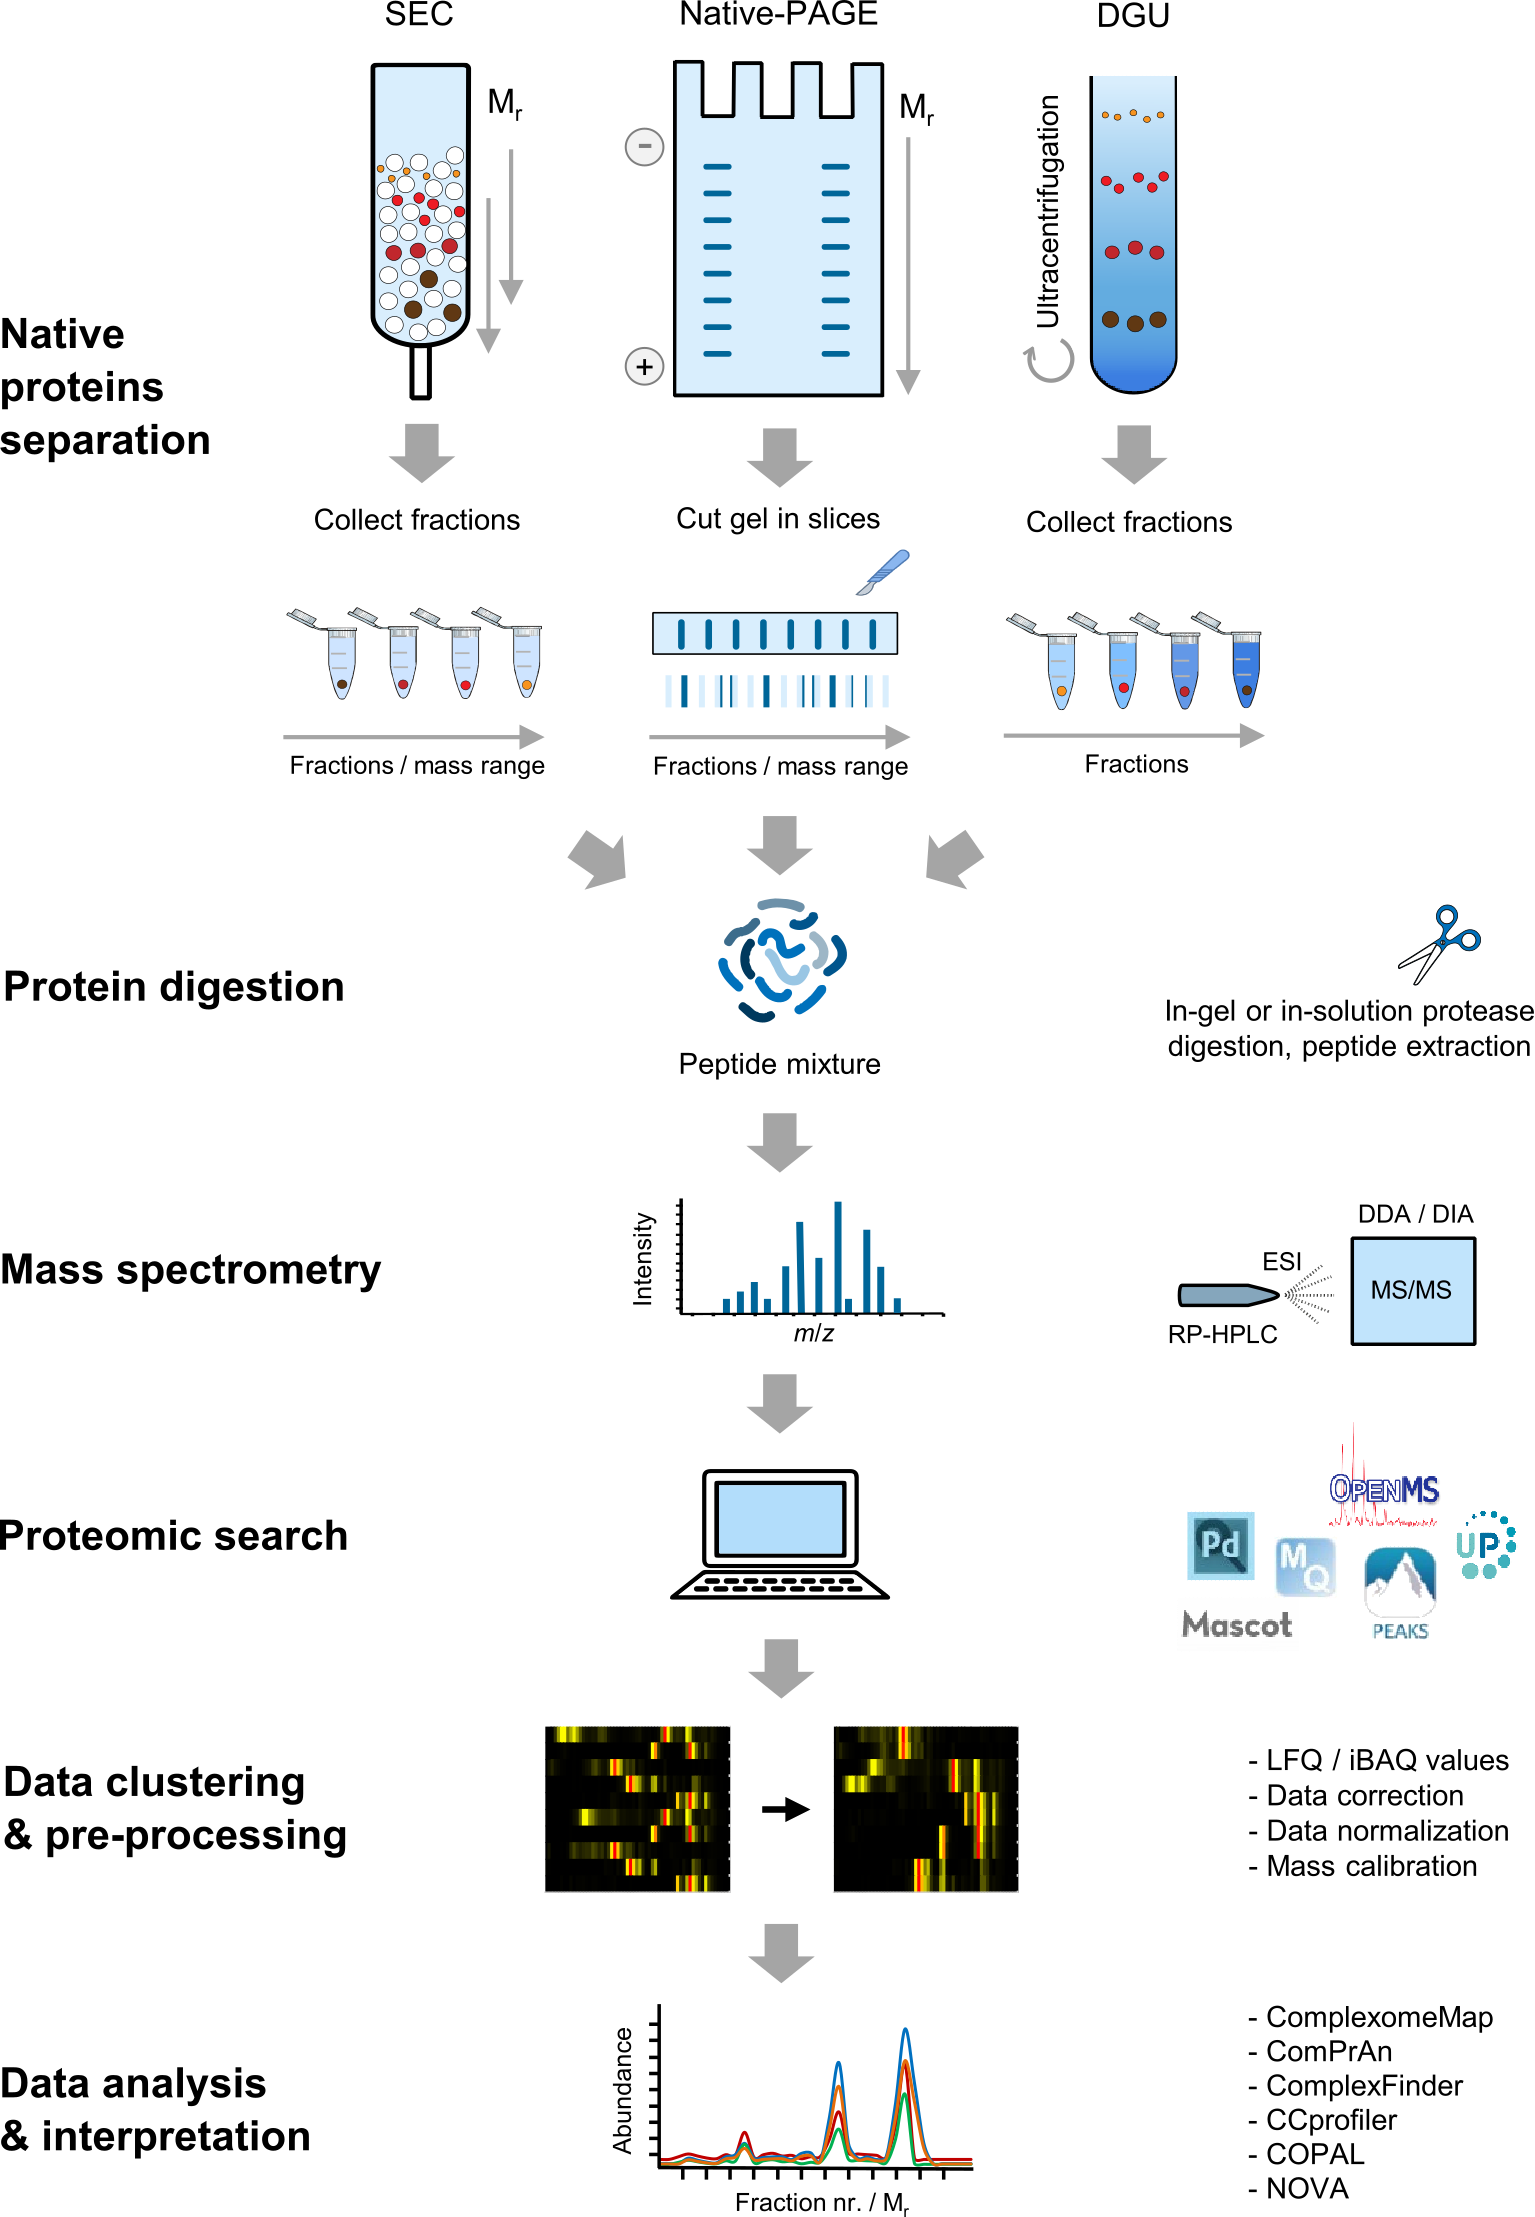
\includegraphics[width=0.9 \textwidth]{Chapter.1/Figures/Figure5.png}
    \caption{Figure Legend on next page}
    \label{fig:fig5}
\end{figure*}
\addtocounter{figure}{-1}
\begin{figure*}[ht!]
    \caption{\textbf{Overall workflow of complexome profiling (CP).} After collection, homogenization and fractionation of biological materials, proteins are separated by either native polyacrylamide gel electrophoresis (PAGE), size exclusion chromatography (SEC) or density gradient ultracentrifugation (DGU) for CP studies. The obtained protein-containing fractions are individually digested with specific proteases. Resultant peptides are extracted, cleaned and usually separated by reversed-phase high-performance liquid chromatography (RP-HPLC) followed by tandem mass spectrometry (MS/MS) analysis. MS data can be acquired in data-dependent or data-independent modes, DDA or DIA, respectively. Next, a proteomic search is performed to match obtained MS spectra against proteome databases using a variety of available software. Icons of the most popular tools used for CP studies are shown (see \textbf{\autoref{sec:CP_MS_intro}}). Protein abundance profiles are further obtained by plotting LFQ/iBAQ values against the number of fractions. The list of identified protein groups is computationally sorted based on similarities of the abundance patterns across fractions; e.g. hierarchical clustering. Prior to analysis, complexome data are pre-processed to account for protein loading/MS sensitivity differences. Data correction and normalization between samples are regularly applied. In SEC- and native-PAGE-based CP, a mass calibration can be implemented for a more meaningful biological dimension. Data can be analyzed by using available bioinformatic tools specifically created for CP (see \textbf{\autoref{ssec:CP_MS_ssec2}}). Some of these programs are shown in the figure. Figure adapted from \cite{Cabrera-Orefice_2022}.}
\end{figure*}
Proteins that are part of the same complex consistently cluster together since these show co-migration in the same fraction(s) and similar abundance profiles.
%
\subsection*{Different complexome profiling set-ups, one common goal}\label{ssec:CP_MS_ssec1}
As a ground-breaking “-omics” method, CP has been rapidly developing and spreading among the scientific community. It is thus not striking that in less than a decade, multiple strategies have complemented or even improved its scope. At the same time, several limitations of CP have been circumvented gradually by including novel MS-based strategies, specific adaptions in sample processing and new tools for data analysis. All variants of CP do share a common goal nonetheless: to unravel the composition of protein complexes, as well as their abundance, stabilities, apparent molecular masses and stoichiometries.\\
The most used CP workflow, currently referred to as “classic CP” \cite{Wittig_2021}, uses Blue Native-polyacrylamide gel electrophoresis (BN-PAGE) followed by MS identification. The main advantages of BN-PAGE are the relatively low amounts of biological material required and high-resolution separation of native proteins. BN-PAGE conditions keep proteins in similar native states to those occurring \emph{in vivo} \cite{Wittig_2006}. However, if the presence of Coomassie blue dye affects the stability of one or more protein complexes of interest, milder dye-free versions of native-PAGE can easily be used instead; e.g., high-resolution clear native-PAGE (hrCN-PAGE) \cite{Ladig_2011, Wittig_2007}. Native-PAGE is suitable for separation of proteins between $\sim$0.02-10 MDa. If the study requires interrogation of bigger protein complexes (>10 MDa), large pore BN-PAGE (LP-BN-PAGE) can be applied instead \cite{Heide_2012, Strecker_2010}.

After electrophoresis, entire gel strips are fixed and often cut into 32-70 slices followed by LC-MS/MS identification \cite{Giese_2021, Heide_2012, Senkler_2017, Vidoni_2017}. For CP analysis, slice numbers can be transformed into apparent molecular mass values by carrying out a calibration using standard proteins as exemplified in \cite{Heide_2012, Wittig_2010}. Molecular mass accuracy is optimized by using different sets of standard protein complexes, one for water-soluble proteins and the other for membrane proteins. On the whole, the more fractions collected the better resolution of the resultant profiles will be. In 2016, Müller and co-workers developed cryo-slicing Blue Native-Mass Spectrometry (csBN-MS), which helped increase the resolution, accuracy and quantification of the complexome profiles by slicing the BN-lanes in 230 pieces as well as optimizing MS analysis and protein identification \cite{Muller_2016}. The resolution of complexome profiles obtained from \(\leq\) 30 slices would not be suitable to unambiguously assign protein interactions.

Besides native-PAGE, size exclusion chromatography (SEC) and density gradient ultracentrifugation (DGU) have been implemented in different CP setups. Using SEC, native proteins are separated by filtration through a gel matrix (resin), which consists of spherical porous beads of different sizes depending on the desired range of molecular masses \cite{Burgess_2018}. Elution of heavier proteins is faster than the lighter ones by this method. Apparent molecular masses of eluted fractions can be determined with proper standard mixes; although the mass calibration is more accurate for globular proteins \cite{Hong_2012, Korepanova_2012}. SEC resins are suitable for separating proteins in a wide range of molecular masses; e.g. 1-700 kDa (SephadexTM, SuperdexTM); 5-5000 kDa (SuperoseTM) and 0.01-40 MDa (SepharoseTM). The number of fractions that can be collected after SEC is comparable to those aforementioned. For example, in the recently introduced SEC-SWATH-MS approach \cite{Heusel_2019}, 81 fractions were collected, subjected to MS identification and examined by complex-centric proteome analysis. This CP setup led to higher sensitivity and accuracy in protein quantification, less noise, and validation of protein interactions. SEC has been particularly useful in CP studies characterizing large protein complexes, such as nuclear components \cite{Connelly_2018}. However, key limitations of SEC-involving CP setups would be the larger amounts of biological material required, loss of protein interactions by dilution, formation of self-oligomers and inadequate identification of membrane and low abundant protein complexes \cite{Burgess_2018, Heusel_2019, Iacobucci_2021}.

On the other hand, DGU uses solutions of different densities made of glycerol, sucrose, cesium chloride, iodixanol or Ficoll\textsuperscript{®} through which protein complexes are separated based on their sedimentation rates, where heavier complexes sediment faster. DGU is an excellent technique for separating large protein complexes, ribosomes, membrane vesicles and subcellular organelles. DGU is also suitable to separate cleared cell lysates as well as immunoprecipitation (IP)-captured protein complexes \cite{Caudron-Herger_2019, Lee_2013}. After separation, most of resolved protein complexes remain in near-native states. In a recent study, a reliable DGU-based CP variant, referred to as quantitative density gradient analysis by mass spectrometry (qDGMS) has been developed to study the human mitoribosome \cite{Palenikova_2021a}. qDGMS combines stable isotope labeling by amino acids in cell culture (SILAC) and DGU followed by fractionation and LC-MS/MS analysis. SILAC is a MS-based technique that quantifies the differences in protein abundance/expression among biological samples \cite{Ong_2002}. In conventional SILAC, two different cell lines/strains are cultured using media supplemented with either “heavy” or “light” essential aminoacids that are labeled with non-radioactive isotopes (e.g., 13C, 2H, 18O, 15N) or unlabeled, respectively \cite{Geiger_2011}. The specific labeled aminoacids are hence incorporated into all cell proteins during cell growth. Proteins of cell lysates/fractions obtained from the two samples are mixed (1:1), digested and analyzed together by LC-MS/MS. The isotope-labeled peptides appear in MS spectra as pairs with identic chemical composition but different masses. Ratios of intensities for the many identified peptide pairs thus denote the respective changes in protein abundance between samples. Incorporation of SILAC not only in qDGMS but also in classic CP allows duplexing, MS time-saving and, most important, higher accuracy of quantification in proteomic analysis of two experimental conditions \cite{Palenikova_2021a, Palenikova_2021b}.

A major challenge of DGU relies on retrieving of fractions without manual disturbance of the resolved layers. To account for this issue, several strategies and devices have been developed, including commercially available automatic fractionators and freezing the gradient after centrifugation followed by cryo-slicing to fractionate samples consistently \cite{Yu_2016}. Location of resolved proteins by DGU is considerably more spread when compared to native-PAGE or SEC, which means that increasing the number of fractions does not necessarily lead to higher resolution. Furthermore, sedimentation rates do not only depend on molecular masses of protein particles but also on shape and densities from both the particles and fluid used for making the gradient \cite{Cole_2008}. For these reasons, co-migration of identified proteins by this CP setup does not immediately represent actual associations rather than merely similar sedimentation rates.
%
\subsection*{Complexome profiling data analysis and visualization} \label{ssec:CP_MS_ssec2}
Huge output files are obtained in CP studies after protein searches, which usually contain all data necessary for further analysis, including identified protein groups, unique peptides, sequence coverage, MS/MS counts, scores, LFQ/iBAQ values from each fraction, etc. The most common visualizations of a complexome profile are heatmaps accompanied by line charts plotting the LFQ/iBAQ values throughout the fractions. Complexome profiles of a short set of proteins can be manually generated and analyzed. Yet, the large volume of protein identifications in CP datasets makes full manual inspection impractical. In the last years, several tools have been specifically designed for automated processing and exploration of CP datasets.
ComplexomeMap has been developed as an online public platform for mining the mitochondrial complexome of plants \emph{Arabidopsis thaliana} and \emph{Viscum album} \cite{Senkler_2017}. NOVA is a user-friendly software to perform cluster analysis, mass calibration, normalization, visual inspection, links to protein databases and comparison of experimental conditions \cite{Giese_2015}. The software COPAL has proven helpful for analyzing multiple CP datasets, aligning experimental replicates and detecting significantly affected protein complexes \cite{Van_Strien_2019}. It also generates files that can be directly used for gene set enrichment analysis. ComPrAn, a Shiny R app, has been developed for analyzing qDGMS data; this tool enables analysis of peptide-level data, normalization, clustering, visualization options and a graphical user interface \cite{Palenikova_2021a}. In addition, ComPrAn is particularly useful to analyze proteomic data obtained from SILAC-treated samples. ComplexFinder, a Python-based software suit, has recently been released to analyze fractionation of native protein complexes, particularly from BN-PAGE- or SEC-based CP experiments \cite{Nolte_2021}. This tool allows machine learning-based prediction of potential protein-protein interactions (PPIs) and high flexibility in CP data analysis. ComplexFinder also provides improved peak-centric quantification and kinetic modelling, protein connectivity networks and compatibility with different quantification strategies. CCprofiler is a robust R package for analyzing co-fractionation MS datasets, which has been originally designed for SEC-SWATH-MS \cite{Heusel_2019}. CCprofiler and its web interface, SECexplorer, offer multiple functions, such as quality control and filtering for less erroneous assignment of protein interactors, usage of curated reference datasets, protein quantification, protein- and complex-centric data analysis and visualization.
Other software available for proteomic and interactome analysis can also be used for CP data processing. For instance, free tools such as Perseus \cite{Tyanova_2016b}, PrInCE \cite{Stacey_2017} and EPIC \cite{Hu_2019} may provide suitable options for visualization, protein quantification, statistical analysis, prediction of PPIs from co-fractionation data, obtention of supporting info from public repositories and/or cross-omics comparisons.
%
\subsection*{Complexome profiling as a tool to investigate mitochondrial protein complexes} \label{ssec:CP_MS_ssec3}
Complexome profiling as a tool to investigate mitochondrial protein complexes
Mitochondria are traditionally known as the eukaryotes` “powerhouses” since they contain all the enzymes required to generate ATP via the oxidative phosphorylation (OXPHOS) pathway. This process is catalyzed canonically by four respiratory chain complexes (I, II, III and IV) and a F1FO-ATP synthase (complex V). Complexes I, III and IV couple the energy released during electron transfer to oxygen to the generation of an electrochemical gradient of protons across the inner mitochondrial membrane (IMM). The proton gradient not only drives the synthesis of ATP, but also other processes such as metabolite transport, protein import, redox and Ca2+ homeostasis, fusion/fission, signaling and cell death. These organelles do also contain their own genome, also known as mitochondrial DNA (mtDNA), which encodes for a few but essential subunits of OXPHOS complexes. The roles of mitochondria are thus not limited to their energy duties. These organelles are multi-functional “hubs” critical to almost every cell process.
Despite of the great progress in molecular characterization and structure elucidation of numerous mitochondrial protein complexes, mostly OXPHOS- and mitoribosome-related proteins, a large number of mitochondrial PPIs remain elusive. In the last years, however, CP has proven valuable for identifying novel protein interactors, validating previous results and shedding light on intricate assembly pathways. In this section, we summarize these findings and describe how CP has boosted the analysis of protein complexes in the mitochondrial research field. Expectedly, most of these findings are again related to components or mediators of the assembly of OXPHOS complexes, energy metabolism-linked proteins and mitoribosomes.

The first groups that established CP have also been interested in the many features of OXPHOS and in particular of complex I (CI). CI is the largest redox enzyme of the mitochondrial respiratory chain constituted by $\sim$45 subunits depending on the species. CI generates proton-motive force driven by the transfer of electrons from NADH to ubiquinone \cite{Hirst_2013}. Although the redox features and composition of mitochondrial CI in several species were already known by the start of the 2010s, major queries on this enzyme had yet unresolved: its entire 3D structure, its energy-conversion mechanism and how it assembles. To help tackle the last one, the formal introduction of CP by Heide and co-workers was useful to identify TMEM126B interacting with the known CI assembly factors NDUFAF1, ECSIT and ACAD9 \cite{Heide_2012}. \emph{TMEM126B} knockdown in 143B osteosarcoma cells led to $\sim$95 \% specific decrease in CI-containing supercomplexes, i.e. supramolecular associations of complexes I, III and IV. These results thus proposed TMEM126B as a CI assembly factor. In an earlier report using HEK293 cells, Wessels and co-workers identified with a similar approach two other assembly factors of CI: C6ORF66 and C3ORF60 \cite{Wessels_2009}, currently known as NDUFAF4 and NDUFAF3, respectively. In this study, mitochondrial proteins were separated by BN-PAGE followed by LC-MS/MS identification, but comparison of migration patterns was limited to the use of PCP.

A few years later, a dynamic CP strategy was successfully implemented to describe the step-by-step integration of the subunits, assembly factors and the different assembly intermediates of human CI \cite{Guerrero-Castillo_2017a}. The authors used CP data from time-based mitochondrial translation recovery to describe a number of assembly intermediates of CI accumulating at various timepoints after removal of chloramphenicol, a reversible inhibitor of mitoribosomes \cite{Ugalde_2004}. These data corroborated the long time proposed modular assembly pathway of CI, which basically involves the coordinated formation and pre-assembly of its functional modules, N, Q, PP and PD, before forming the entire enzyme. This study also provided insight into the specific involvement of earlier reported assembly factors and novel interactors. Complex IV (CIV) assembly-related chaperone COA1 and TMEM186 were clearly found associated with membrane arm intermediates that also interact with TMEM126B, NDUFAF1 and ECSIT. At present, all these proteins have been recognized as true components of the so-called mitochondrial CI assembly (MCIA) complex \cite{Formosa_2020}. ATP5SL clustered with FOXRED1, another CI assembly factor. However, ATP5SL disruption did not lead to CI deficiency \cite{Andrews_2013} and its involvement in the assembly pathway is thereby unclear. Complex V assembly-involved protein TMEM70 was also identified in assembly intermediates of CI. To further explore the putative role of TMEM70 on CI assembly, Sánchez-Caballero and co-workers performed a study including proximity-dependent biotin identification (BioID), co-evolution analyses and CP \cite{Sanchez-Caballero_2020}. In this study, TMEM70 was found in close contact with subunits of complexes I and V, as well as the small mitoribosome subunit. The absence of TMEM70 resulted in slight depletion of fully assembled CI and accumulation of assembly intermediates of the distal part of the membrane arm of CI, whereas mature complex V (CV) content was $\sim$70 \% lower than in the control cell line. These authors showed TMEM70 as a non-essential assembly factor of complexes I and V, and proposed a possible role in tethering mitoribosomes to the IMM during translation.
Apart from studies in human cells, CP has also been used to study the role of several accessory subunits of CI in different models. For example, Kmita and co-workers analyzed the assembly of CI in a deletion strain of the yeast \emph{Yarrowia lipolytica} lacking the Zn2+-containing subunit NUMM/NDUFS6 \cite{Kmita_2015}. Absence of this subunit did not prevent formation of the entire CI, since a lower enzyme content and higher fraction of peripheral arm subcomplexes were observed. Unexpectedly, the almost fully assembled CI contained the assembly factor N7BML/NDUFAF2 bound instead of accessory subunit N7BM/NDUFAF12. Moreover, Angerer et al. implemented CP in a study on the mitochondrial acyl carrier proteins (ACPM) 1 and 2, which are accessory subunits of CI and contain LYR motifs \cite{Angerer_2014}. Although ACPM1/2 are predominantly associated to CI, ACPM1 was also found as a free protein in the matrix and forming a complex with LYRM4(ISD11)/NFS1 involved in iron-sulfur cluster biosynthesis. Furthermore, two different groups in parallel unveiled the existence of two isoforms of the peripheral arm subunit NDUFV3 of CI in mammals \cite{Bridges_2017, Guerrero-Castillo_2017b}. An extra exon present in gene \emph{NDUFV3} can be alternative spliced, hence generating short and long isoforms of $\sim$10 and $\sim$50 kDa, respectively. CP helped find a different expression of these isoforms in different tissues of bovine, mouse and rat as well as in cultured human cells. The canonical short isoform was predominantly identified in heart and skeletal muscle, whereas the large isoform was the foremost isoform in liver, brain and lung tissues. Both NDUFV3 isoforms can also be expressed at the same time and correctly assembled onto CI in some tissues; yet, one isoform predominated in each case.

Other OXPHOS complexes and their chaperones have also been explored by CP. Singhal et al. identified the product of ORF \emph{YDR381C-A} as an assembly factor of yeast complexes III and IV \cite{Singhal_2017}. This protein was renamed as cytochrome \emph{c} oxidase interacting protein 1 (Coi1), which occurs only in fungi. Deletion of Coi1 resulted in severe alteration of mitochondrial function, diminished amounts of CIV-associated heme, defective assembly of complexes III, IV and their supercomplexes, as well as accumulation of assembly intermediates. Vidoni and co-workers reported that the short isoform of myofibrillogenesis regulator 1 (MR-1S) associates with chaperones PET100 and PET117 to mediate human CIV assembly \cite{Vidoni_2017}. Authors implemented not only CP to study assembly intermediates accumulated in control and \emph{MT-CO3} mutant cybrids, but also SILAC and quantitative MS.\\
CP has been helpful to better understand the formation of supercomplexes or respirasomes. The specific factors for mediating this process remain unclear. COX7A2L, also known as SCAFI, has been shown critical for the association of complexes III and IV \cite{Perez-Perez_2016}. Its putative involvement in larger respirasome formation has also been reported \cite{Lapuente-Brun_2013}. To better understand the role of SCAFI, Férnandez-Vizarra et al. explored the mitochondrial complexome of a SCAFI knockout human cell line by SILAC-based CP \cite{Fernández-Vizarra_2021}. Absence of SCAFI resulted in marked loss of supercomplex III2-IV, whereas CI-containing respirasomes were not affected. In contrast, authors showed that $\sim$70 \% of respirasomes contained COX7A2 in either human cell line analyzed. This discrepancy has apparently been related to a tissue-specific expression of the two isoforms \cite{Lapuente-Brun_2013}. On the other hand, Protasoni and co-workers demonstrated that absence of a fully assembled complex III (CIII) in a MT-CYB-deficient human cell line stalled CI biogenesis by preventing the integration of its N-module \cite{Protasoni_2020}. Although substantial accumulation of partially assembled Q/P intermediate was observed by SILAC-based CP, a slight fraction of CI could still be detected. Reasonably, respirasome assembly was totally lost in the mutant. Besides, assembly of CIV was affected since several COX subunits were found associated with CIII sub-assemblies; hence interfering their correct assembly. It has thus been proposed that human complexes I, III and IV assemble in a cooperative fashion, where CIII seems to be central.

Mitochondria are characterized by a highly folded IMM. These folds, called cristae, have emerged as dynamic compartments whose shape and dimensions influence structure and functioning of the OXPHOS system \cite{Cogliati_2016}. A key player in shaping cristae appears to be the MICOS complex, which also interacts with the sorting and assembly machinery (SAM) complex from the outer mitochondrial membrane (OMM) \cite{Huynen_2016}. Interaction of these two complexes constitutes the mitochondrial intermembrane space bridging (MIB) complex \cite{Ott_2015}. Since its relatively recent discovery \cite{Harner_2011}, much of what we know about the MICOS complex has been derived from CP-based studies. For instance, Weber and co-workers identified apolipoprotein O (APOO/MIC26) and apolipoprotein O-like protein (APOOL/MIC27) as potential components of the human MIB complex \cite{Weber_2013}. Huynen and co-workers described the composition and apparent masses of the fully assembled MIB complex (2.2-2.8 MDa) and other putative assembly intermediates, e.g. the free MICOS complex ($\sim$700 kDa) \cite{Huynen_2016}. Anand et al. identified MIC13 (QIL1) as a novel MICOS complex subunit \cite{Anand_2016}. Deletion of MIC13 resulted in a smaller albeit still assembled MICOS complex while having no effect on integrity of OXPHOS complexes. They also demonstrated a disruptive effect of MIC13 deletion on cristae morphology accompanied by reduced respiratory capacity. The same group used a similar approach to characterize MIC26 and MIC27 \cite{Anand_2020}. They showed negative effects on CV stability as well as cristae morphology defects both of which were much more pronounced in the double knockout than either single knockout, suggesting overlapping roles. Assembly of other MICOS components was however unimpeded by MIC26/27 knockouts, proposing these proteins are not essential for its assembly or stability. The link of MICOS components to CV was further explored by Eydt and co-workers \cite{Eydt_2017}, showing that MIC10 comigrates with CV dimers. Additionally, they presented evidence that MIC10 acts antagonistically to MIC27 in negatively controlling CV oligomerization, while MIC27 appears to be a positive regulator. A recent paper by Bock and co-workers reported the interaction of  PGC-1- and ERR-induced regulator in muscle 1 (PERM1) with multiple components of the MICOS/MIB complex as well as vimentin and ankyrin B in skeletal muscle from mouse \cite{Bock_2021}. These findings suggested a novel mechanism to help understand not only the interconnection of mitochondria and sarcolemma but also mitochondria-cytoskeleton associations as well as the organization of a functional mitochondrial network in this tissue. Taken together CP has greatly aided our understanding of MICOS/MIB complex composition, the role of individual subunits and its interaction with OXPHOS complexes.

The IMM contains other key protein complexes involved in proteolytic events, fusion/fission of mitochondrial membranes, regulation of cristae morphology and cell signaling. Some of these proteins belong to the SPFH (stomatin, prohibitin, flotillin and HflC/K) family and usually arrange as large scaffolds. To have a clearer picture, Wai and co-workers implemented CP to unveil the interaction partners of stomatin-like protein 2 (SLP2) and at least two proteases, PARL and YME1L, in immortalized embryonic fibroblasts mitochondria \cite{Wai_2016}. SLP2 works as a regulator of PARL, which also modulates other proteins such as PGAM5, PINK1 and OMA1. These interactions were suggested to occur in defined sites of the IMM and related to mitochondrial proteostasis, dynamics and cell survival. Similarly, Konig and co-workers identified MAIP1 (C2Orf47) as a novel \emph{m}-AAA protease-binding protein in complexome profiles \cite{Konig_2016}. MAIP1 was shown essential for regulating the assembly of subunit EMRE into mitochondrial Ca2+ uniporter (MCU) complexes.

CP has also played an important role in the field of plant and parasite mitochondrial biology. Using CP, Senkler and co-workers performed a systematic characterization of mitochondrial complexes in the plant \emph{Arabidopsis thaliana} \cite{Senkler_2017}. CP data were also useful to update the subunit composition of OXPHOS complexes and identifying respective assembly intermediates. This group then used the same approach on mitochondria from the mistletoe \emph{Viscum album}, revealing a highly unusual OXPHOS system \cite{Senkler_2018}. This species completely lacks CI, the only multicellular eukaryote to date with this distinction; instead, \emph{Viscum album} contains alternative NAD(P)H oxidoreductases. This species also expresses an alternative oxidase and its complexes III and IV are firmly associated as supercomplexes. In comparison to \emph{Arabidopsis thaliana}, the abundance of complexes II and V was particularly low, suggesting a shift in stoichiometry of the OXPHOS complexes in the IMM of this plant. Rugen and co-workers took a more focused CP strategy to investigate the composition of the mitoribosome in \emph{Arabidopsis thaliana} \cite{Rugen_2019}. Utilizing LP-BN-PAGE- and DGU-based CP setups, several non-conventional proteins were found attached to the mitoribosome, mostly from the class of pentatricopeptide repeat proteins that seem to be involved in RNA processing and protein maturation. Presence of these additional interactors results in a larger mitoribosome with unusual large and small subunits of $\sim$3 and $\sim$5.7 MDa, respectively. Additional functions are thus likely incorporated into the plant mitoribosome.

Due to their extreme divergence, apicomplexan parasites of the genera \emph{Plasmodium} and \emph{Toxoplasma} that cause the infectious diseases malaria and toxoplasmosis, respectively, remain poorly understood. In fact, more than one-third of their genes still lack any functional annotation \cite{Aurrecoechea_2009, Harb_2020}. To help narrow this gap, Evers et al. and Maclean et al. obtained evidence for highly divergent composition of the mitochondrial OXPHOS complexes in \emph{Plasmodium falciparum} and \emph{Toxoplasma gondii}, respectively \cite{Evers_2021, Maclean_2021}. More than 30 novel subunits across complexes II, III, IV and V with no recognizable orthologs outside of the myzozoan phylum could be identified by CP. These novel subunits did not only replace subunits typically observed in standard models, but also increased the size of \emph{Plasmodium falciparum} OXPHOS complexes by around 50 \%, 50 \%, 130 \% and 70 \% as compared to complexes II, III, IV and V from mammalian mitochondria, respectively. This was consistent with the observations in \emph{Toxoplasma gondii}, thus making apicomplexan OXPHOS complexes the largest described to date. Furthermore, abundance of OXPHOS complexes was $\sim$32 fold increased in the transmissible gametocyte stages compared to the pathogenic asexual stages of \emph{Plasmodium falciparum} \cite{Evers_2021}. This finding offered protein-level support for the long-standing hypothesis that malaria parasites undergo a metabolic switch towards mitochondrial catabolism to facilitate their transmission back to the insect vector \cite{MacRae_2013}. Despite its relatively recent introduction to the field of parasite research, CP has already provided valuable data for mapping a number of previously unknown interactors to protein complexes and biological processes. As these novel additions are unlike what is known from standard models, it opens the door for new discoveries, even in pathways as fundamental as respiration.
%
\section{Combining XL-MS and CP-MS for the structural analysis of protein complexes in mitochondria}
Over the last decade, through advances in mass spectrometry, chemical cross-linkers and data base search strategies cross-linking mass spectrometry (XL-MS) has emerged as a powerful technology for interactome and structural biology studies in mitochondria \cite{Hevler_2021b, Liu_2018, Ryl_2020, Schweppe_2017}. Notwithstanding, the diverse protein complex landscape within mitochondria, where some proteins are found across several co-occurring complexes (e.g. respiratory super-complexes) \cite{Letts_2016, Rugolo_2021, Schägger_2000, Wu_2016}, substantially complicates the structural analysis. While XL-MS provides information about physical interactions within a complex, its exact stoichiometry cannot be confidently assigned. Knowing the exact stoichiometry of a complex is essential to guarantee accurate cross-linking guided structural modeling of protein complexes. For this reason, CP and XL-MS are highly complementary and could provide valuable insights into the macromolecular organization of the mitochondrial complexome. As shown in chapter 2 of this thesis, combining CP and XL-MS data enabled detailed atomic modeling of monomeric complex IV (COX) associated with dimeric apoptosis-inducing factor 1 (AIFM1) \cite{Hevler_2021b}. CP analysis was indeed helpful to determine the stoichiometry of this complex and validating the interaction. Combination of both approaches offers the possibility to cross-validate PPIs and to identify protein complexes that could be overlooked otherwise. Although actual scalability and throughput have not yet been addressed, combination of CP and XL-MS holds a great potential not only to better define the composition and states of protein complexes but also to help stabilize transient PPIs.

Besides knowing the exact complex stoichiometry, determination of the optimal concentrations of cross-link reagent and protein is strictly required to abate artifacts. To help circumvent this, in chapter 3 we describe a hybrid workflow termed in-gel cross-linking (IGX-MS) \cite{Hevler_2021a}. In this method, proteins are separated by BN-PAGE and the gel spots of interest are cut and incubated with a cross-linker, digested and further analyzed by LC-MS/MS. IGX-MS not only makes time-consuming experimental optimization steps (e.g. determining concentration of cross-linkers, optimal buffer system, etc.) nearly obsolete but also decreases the required protein amounts as well as undesired over-length cross-links. In contrast to classical in-solution XL-MS workflows, IGX-MS allows the differentiation of conformation- and interaction-specific distance restraints as it has been shown for various mitochondrial complexes but also for plasma protein complexes, the mitotic checkpoint complex (MCC) as well as for different assemblies of the archaeal ammonia monooxygenase \cite{Fischer_2022, Hevler_2021a, Hodgskiss_2022, Lukassen_2021}. IGX-MS seems specially promising for future modeling studies that aim at characterizing co-occurring protein complexes with different stoichiometries or assembly states.
XL-MS has also been used to validate another CP-like setup that includes protein separation by SEC, quantitative MS analysis, cryo-electron microscopy (EM) and computational modeling. This structural proteomics approach allowed simultaneous description of the abundance, PPIs and structure profiling of 1/3 of the proteome of \emph{Chaetomium thermophilum} \cite{Kastritis_2017}. These results were integrated in a network map comprising 48 protein complexes and communities. This approach was also suitable to resolve the structure of the fatty acid synthase complex and its arrangements. Recent inclusion of image-processing workflows based on machine-learning methods opens the door to a much more robust data analysis, improved identification of PPIs, higher resolution in structure models and multi-scale molecular description of protein communities in situ \cite{Kyrilis_2021a}.
\newpage
\section*{References}
\bibliographystyle{Style_settings/bibstyle_pnas}
\bibliography{Chapter.1/chapter1_bib_form}


\chapter{\large Selective cross-linking of coinciding protein assemblies by in-gel cross-linking mass-spectrometry} \label{ch-2}

\begin{center}
\vspace{0.5cm}     
\footnotesize
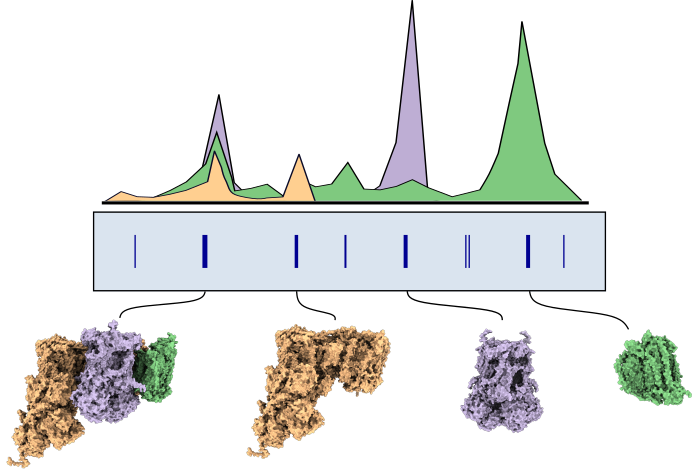
\includegraphics[width=0.5\textwidth]{Chapter.2/Figures/chapter_cover.png}
\vspace{1cm}

{Johannes F. Hevler\textsuperscript{*}, Marie V. Lukassen\textsuperscript{*}, Alfredo Cabrera-Orefic, Susanne Arnold, Matti F. Pronker, Vojtech Franc and Albert J.R. Heck}
\end{center} 

\begin{flushleft}
\vspace*{\fill}    
\rule{\textwidth}{1pt}\\[0cm]
\textbf{This chapter is based on work in the following publication:}\\
\footnotesize
\textbf{\emph{The EMBO Journal}} (2021), 40:e106174, doi:10.15252/embj.2020106174\\

\footnotesize
\vspace{0.3cm}
\begin{tabular}[t]{p{0.01\textwidth}p{0.90\textwidth}}
\textsuperscript{*} & These authors contributed equally to this work\\
\end{tabular}
\end{flushleft}

\newpage
\begin{abstract101} 
Cross-linking mass spectrometry has developed into an important method to study protein structures and interactions. The in-solution cross-linking workflows involve time and sample consuming steps and do not provide sensible solutions for differentiating cross-links obtained from co-occurring protein oligomers, complexes, or conformers. Here we developed a cross-linking workflow combining blue native PAGE with in-gel cross-linking mass spectrometry (IGX-MS). This workflow circumvents steps, such as buffer exchange and cross-linker concentration optimization. Additionally, IGX-MS enables the parallel analysis of co-occurring protein complexes using only small amounts of sample. Another benefit of IGX-MS, demonstrated by experiments on GroEL and purified bovine heart mitochondria, is the substantial reduction of undesired over-length cross-links compared to in-solution cross-linking. We next used IGX-MS to investigate the complement components C5, C6, and their hetero-dimeric C5b6 complex. The obtained cross-links were used to generate a refined structural model of the complement component C6, resembling C6 in its inactivated state. This finding shows that IGX-MS can provide new insights into the initial stages of the terminal complement pathway.
\end{abstract101}

\newpage

\section{Introduction}
Over the last decades, bimolecular mass spectrometry (MS), with its ability to analyze low amounts of samples with high speed and sensitivity, has evolved into a central pillar beneficial for integrative structural biology \cite{de_Souza_2020, Kaur_2019, Lossl_2016, Robinson_2019}. The structural MS toolbox contains multiple complementary approaches. Next to native MS and top-down MS, a variety of peptide-centric MS methods, such as thermal proteome profiling (TPP), limited proteolysis (LiP), hydrogen/deuterium exchange (HDX) MS and chemical cross-linking MS (XL-MS or CLMS), have emerged and enabled structural studies of a wide range of biomolecules \cite{Feng_2014, Heck_2008, Leitner_2010, Savitski_2014, Zheng_2019}. With recent advances in instrumentation, sample preparation, and data analysis, especially XL-MS has started to fulfill its potential to complement well established structural methods such as X-ray crystallography, nuclear magnetic resonance spectroscopy (NMR), and cryo-electron microscopy (cryo-EM) \cite{Leitner_2016, Matthew_Allen_Bullock_2016, Rappsilber_2011}. XL-MS has a particular utility to capture protein-protein interactions in solution by measuring spatial distance restraints, mirroring structural conformations of intact proteins. Concomitantly, a wide range of chemical cross-linkers have been explored so far, often relying on similar chemical principles \cite{Sinz_2003, Steigenberger_2020}. Most used cross-linkers are small, homo-bifunctional reagents, with two reactive moieties capable of covalently binding two nearby amino acids. The reactive groups are separated by a spacer arm of varying lengths, which can be gas-phase cleavable or non-cleavable, thereby determining different MS data acquisition methods \cite{Kao_2011, Leitner_2010, Muller_2010, Staros_1982}. Recent advances in search engines for more efficient identification of cross-linked peptides allowed structural studies of purified proteins or protein complexes, as well as large scale experiments with more complex samples like purified organelles or cell lysates, using buffer systems which aim to meet physiological relevant conditions \cite{Beveridge_2020, Chen_2019a, Gotze_2019, Klykov_2018}. A typical XL-MS workflow begins with the optimization of the cross-linker concentration. Next, a protein mixture is incubated with the cross-linking reagent, and the reaction is subsequently quenched to prevent the generation of unwanted random protein contacts. After (tryptic) digestion, cross-linked peptides are subjected to various pre-fractionation steps or enrichment strategies to distinguish them from the vast majority of unmodified peptides. Cross-linked residues are eventually identified using dedicated XL-MS search algorithms, providing structural information in the form of distance restraints, which can be utilized to guide computational homology modeling, refinement of flexible regions within structural models, protein-protein docking and the generation of protein interaction networks \cite{Albanese_2020, Bullock_2018, Iacobucci_2019, Kim_2018, Ryl_2020}. Currently, technological developments in XL-MS aim to further improve the cross-linking reaction efficiency and detection. The research is mainly focused on sample preparation techniques, MS fragmentation and enrichment strategies, data acquisition and analysis of cross-linked peptides, as well as the design of novel cross-linkers \cite{Chen_2019b, Dau_2019, Iacobucci_2018, Leitner_2012, Liu_2017, Mendes_2019, Steigenberger_2019}.\\
Although the latest advances significantly revised and reformed the field of XL-MS, some challenges remain. A central problem of XL-MS data analysis is the occurrence of both false-positive and false-negative cross-link identifications. Especially, the existence of proteins with highly dynamic/flexible conformations and the presence of co-occurring alike protein complexes (e.g., protein oligomers and co-occurring complexes sharing distinct sub-units) significantly complicate the analysis by current in-solution XL-MS approaches. Interaction specific cross-links are relevant as structural changes can be triggered by the presence of a binding partner or the environment, thereby eventually displaying a physiological relevant protein conformation \cite{de_Souza_2020, Feng_2014, Mannige_2014, Uversky_2011}. Additionally, when using too high cross-linker concentrations or too high protein concentrations, undesired artificial interactions are likely being picked up by XL-MS. In-solution XL-MS experiments, therefore, need careful experimental optimization of, in particular, the concentration of the proteins and the cross-linker. Unfortunately, these steps require considerable sample amounts (tens of micrograms) and extra experimental time.\\
Here we describe an alternative approach, performing in-gel cross-linking mass spectrometry (IGX-MS), re-discovering the great separation power of gel-electrophoresis. Prior to cross-linking, we load the samples and perform blue native polyacrylamide gel

\begin{figure*}[hbt!]
\center
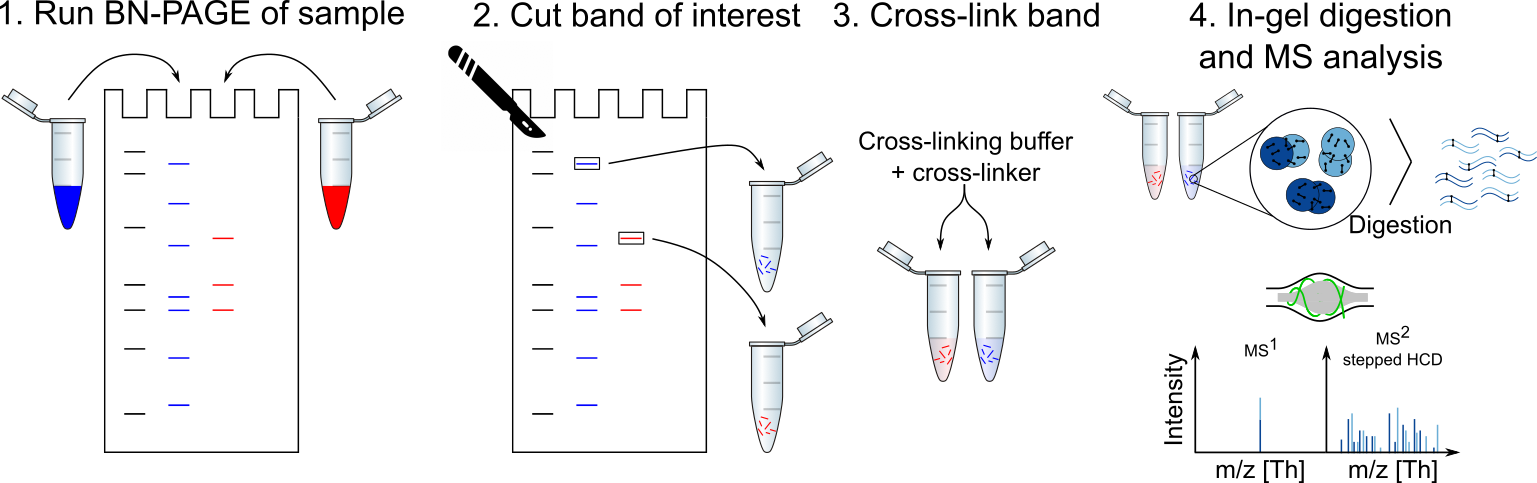
\includegraphics[]{Chapter.2/Figures/Figure1.png} 
\caption{\textbf{Combining BN-PAGE with IGX-MS.} In the first step, proteins and their assemblies are loaded and separated by BN-PAGE. The bands representing different protein assemblies are visualized after running the gel with Coomassie in the upper running buffer. The band(s) of interest are then excised from the gel and incubated with a cross-linking reagent in the cross-linking buffer. The cross-linking reaction is quenched and subsequently subjected to standard in-gel digestion. The extracted peptides are finally analyzed using cross-linking optimized parameters for the MS analysis.}
\label{fig:ch2_fig1}
\end{figure*}

electrophoresis (BN-PAGE), allowing the separation of distinct structural states of the proteins or protein complexes. The distinct bands are subsequently excised and cross-linked in the gel, enabling the measurement of conformation- and interaction-specific cross-links and derived distance restraints (\textbf{\autoref{fig:ch2_fig1}}). We show that this IGX-MS workflow has certain advantages compared to the in-solution based XL-MS methods. These include, amongst other things, no need for cross-linker concentration optimization, generation of conformation-specific cross-links, and relatively low sample amount requirements. Moreover, through IGX-MS data obtained for several protein assemblies, we provide evidence that proteins retain not only their quarternary but also their secondary and tertiary native structural states under BN-PAGE separation. To directly compare IGX-MS with in-solution XL-MS, we selected, as a proof-of-concept, the 14-mer \emph{Escherichia coli} GroEL chaperone and different respiratory chain complexes (super complex 1, complex I and complex V) from solubilized bovine heart mitochondria (BHM). Our experiments demonstrated that IGX-MS can accurately target specific subcomplexes co-existing in the protein complex mixtures and substantially reduce the number of (potentially false) over-length cross-links. Ultimately, we applied the optimized IGX-MS to investigate structures of the terminal complement proteins C5 and C6, which are involved in the initial steps towards the assembly of membrane attack complex (MAC). Our cross-linking data lead us to propose a refined alternative structural conformation of the complement component C6, providing new insights into the terminal complement pathway. In summary, our data show that BN-PAGE-based IGX-MS is a powerful tool, allowing the efficient generation of compositional- and interaction-specific distance constraints, with the potential of refining structural models of a large variety of protein assemblies, even when they co-occur in solution.

\section{Results}
\subsection*{BN-PAGE forms the basis for IGX-MS}
Blue native polyacrylamide gel electrophoresis, BN-PAGE, has proven to be a robust and sensitive method for separating protein complexes from various sample types. It requires only minimal sample amounts to sensitively estimate native protein molecular weights (Mw), respective compositional states, and protein-protein interactions. Further, proteins and protein complexes are thought to maintain not only their overall quarternary structural organization in the gel but also their secondary and tertiary structural organization, as they can still, after that, be subjected to further structural and functional analysis (2D crystallization, cryo-EM, in-gel activity assay) \cite{Poetsch_2000, Schafer_2006, Wittig_2007}.\\
Here, we combine BN-PAGE with XL-MS to efficiently isolate and investigate co-occurring protein oligomeric states and sub-complexes. We first determined whether proteins and protein complexes can be cross-linked in a BN gel. For this, 10 $\mu$g of purified E. Coli GroEL diluted in a Tris buffer was subjected to BN-PAGE as described previously \cite{Wittig_2006}. Bands corresponding to the native 14-mer GroEL (MW = 800 kDa) were excised from the BN-PAGE (\textbf{\autoref{fig:ch2_app_fig1}A}), and further, cut into small pieces and incubated with or without the cross-linker reagent DSS. Next, GroEL was extracted from the gel pieces and subsequently loaded onto a reducing SDS-PAGE (\textbf{\autoref{fig:ch2_app_fig1}B}). The control lane (no cross-linker) revealed only one distinct band at 57 kDa representing the GroEL monomers. In contrast, the BN-PAGE band that was incubated with DSS showed several additional high-molecular-weight bands above 100 kDa, indicating the successful cross-linking of GroEL subunits. Notably, the initial sample buffer (Tris) is incompatible with amine-reactive cross-linkers, as it contains primary amines that compete with the primary amines of Lysine residues, thereby significantly reducing the cross-link efficiency. Successful cross-linking of GroEL in-gel highlights the buffer exchange capacity of the BN-PAGE system, making additional buffer exchange steps (e.g., using molecular weight cut-off filters or dialysis), which would be required for in-solution cross-linking and eventually result in loss of sample, obsolete.

\subsection*{IGX-MS optimization is straightforward}
To prevent protein precipitation caused by over cross-linking, standard in-solution XL-MS crucially depends on using the optimal cross-linker concentration. For this, a subset of sample needs to be incubated with varying cross-linker concentrations prior to the experiment and subsequently analyzed by gel electrophoresis. The time and sample consuming optimization step led us to investigate the effect of varying cross-linker concentrations for IGX-MS experiments. GroEL was subjected to BN-PAGE, and relevant bands were cross-linked using the two different cross-linking reagent DSS and DSSO varying in five concentration steps from 0.5 to 5 mM. After quenching the cross-linking reaction with Tris, the protein-containing bands were prepared for MS analysis following a standard in-gel digestion procedure. Cross-links obtained for DSS and DSSO, and each concentration were validated by mapping them onto the GroEL structure (PDB ID: 1KP8), and lysine C$\alpha$-C$\alpha$ distances were obtained (textbf{Dataset EV1}). The distance distribution for both cross-linkers was highly similar at all used concentrations, and almost no cross-link distances over 30 Å were observed across the varying concentrations, indicating that IGX-MS is highly resistant against over cross-linking of proteins (\textbf{\autoref{fig:ch2_fig2}A}). Our data suggest that IGX-MS is also less hampered by\\

\begin{figure*}[hbt!]
\center
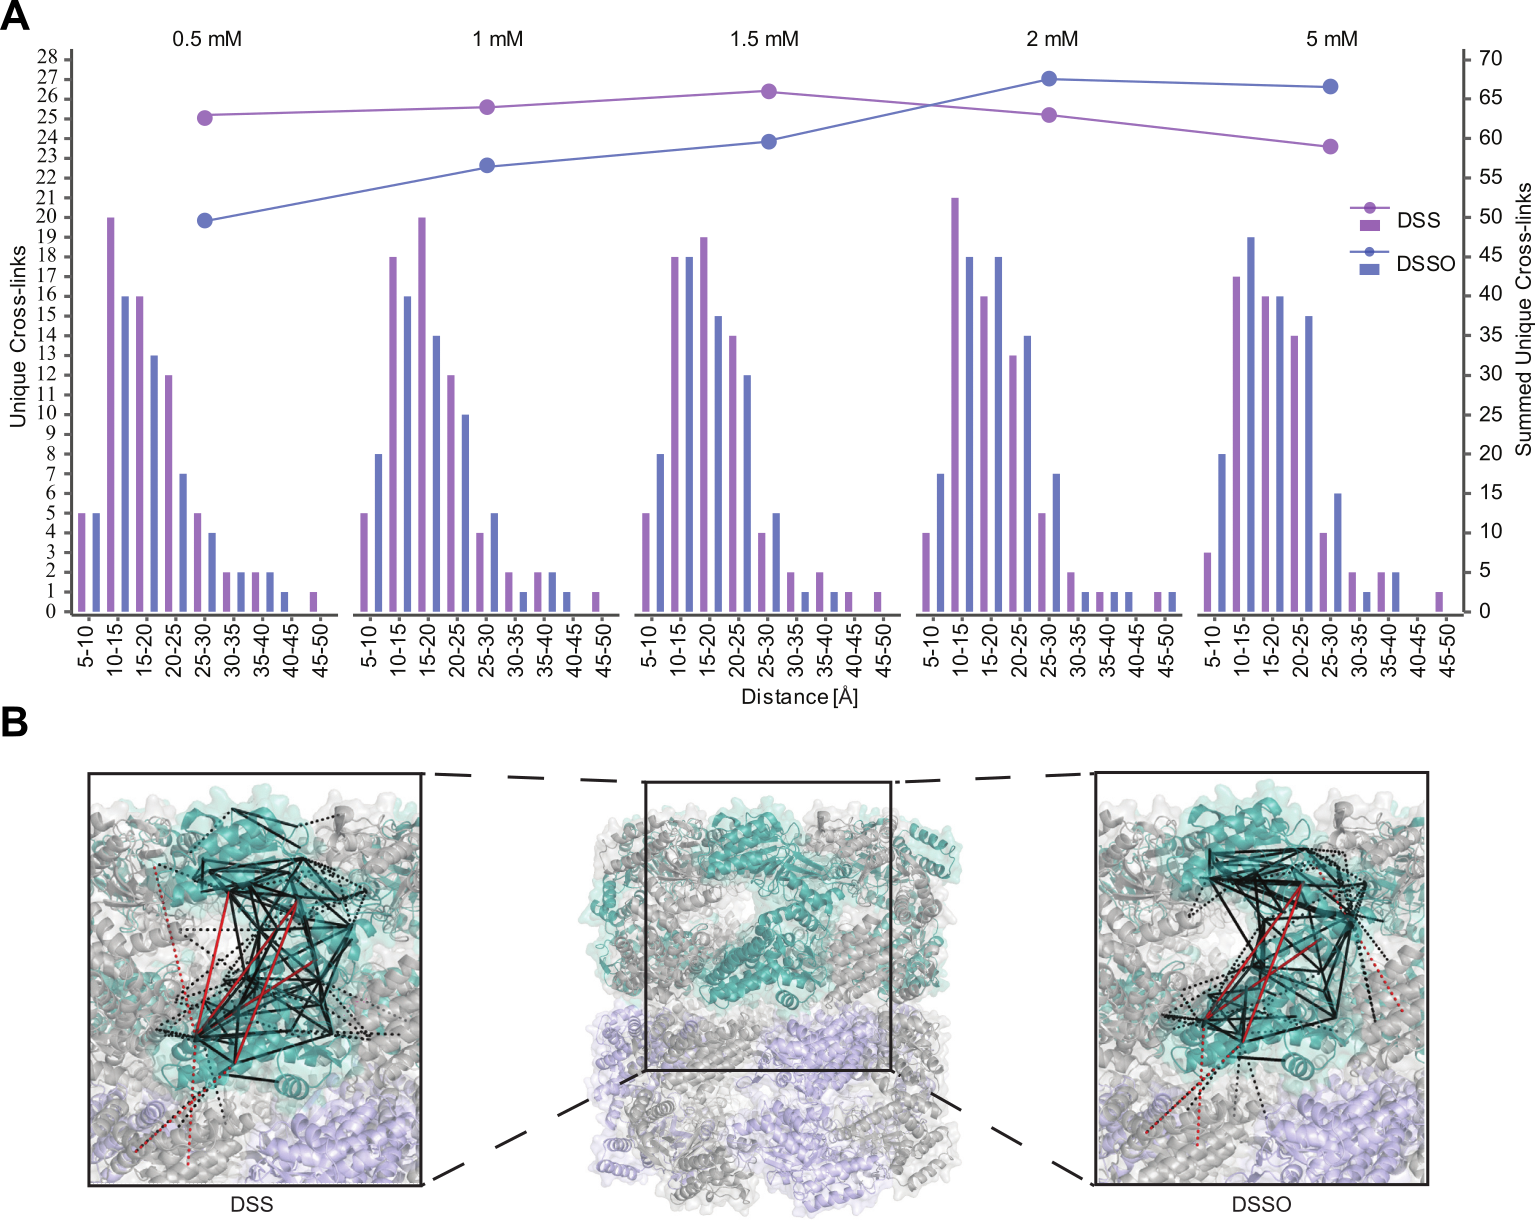
\includegraphics[]{Chapter.2/Figures/Figure2.png} 
\caption{\textbf{IGX-MS of GroEL using either DSS or DSSO at varying concentrations.} \textbf{A.} \emph{Escherichia coli} GroEL was cross-linked by IGX-MS using either DSS or DSSO at concentrations ranging from 0.5 to 5 mM. The identified cross-links were placed on the reported GroEL structure (PDB ID:1KP8), whereby the number of unique cross-linked lysine C$\alpha$-C$\alpha$ distances (using the left y-axis) were binned and as shown in bars. The summed number of unique cross-links obtained at each concentration is shown in lines using the right y-axis. \textbf{B.} Cross-links obtained by IGX-MS using DSS or DSSO plotted onto one subunit of GroEL (intra-links; solid lines) (PDB ID:1KP8) and neighboring subunits (inter-links; dashed lines). Cross-links agreeing with the set distance restraint of 30 Å are colored black, links exceeding the restraint are colored red.}
\label{fig:ch2_fig2}
\end{figure*}

unspecific cross-links. We also observed that the total number of unique cross-links was not affected by the concentration of DSS, and only marginally effected for DSSO as the obtained cross-links are slightly lower for concentrations below 2 mM (\textbf{\autoref{fig:ch2_fig2}A}). However, no significant difference was detected between 2 mM and 5 mM (\textbf{\autoref{fig:ch2_fig2}A}). The cross-linked sites onto the GroEL structure showed good consistency in cross-linked regions for both DSS and DSSO experiments (\textbf{\autoref{fig:ch2_fig2}B}, \textbf{Dataset EV1}). Finally, we compared the cross-linking results for each cross-linker and concentration across the three replicates, demonstrating excellent reproducibility of the IGX-MS experiments (\textbf{\autoref{fig:ch2_app_fig2}}). Based on these results, a DSS concentration of 1.5 mM and a DSSO concentration of 2 mM (\textbf{\autoref{fig:ch2_fig2}A}) were used for the subsequent experiments.

\subsection*{Direct comparison of IGX-MS and in-solution XL-MS}
BN-PAGE facilitates the distinction of oligomeric states, but it can also be particularly useful when protein complexes are reconstituted. In such experiments, one or more of the subunits may be (unwillingly) in excess. These preparations can then lead to false cross-link interpretations, as especially intra cross-links can originate from the free monomer subunit or subunit in the complex (which may exhibit another conformation). By comparing IGX-MS and in-solution XL-MS of GroEL, we aimed to access the relevance of this additional separation aspect and confirm that proteins maintain their native structural integrity during in-gel separation. First, for in-solution cross-linking, GroEL diluted in Tris buffer was buffer exchanged to PBS, and subsequently, the optimal cross-linker concentration was determined by SDS-PAGE to avoid over cross-linking (\textbf{\autoref{fig:ch2_app_fig3}A}). Next, the in-solution XL-MS sample was cross-linked with DSS, while the IGX-MS sample was cross-linked with both DSS and DSSO. Subsequent comparison of DSS- and DSSO-in-gel cross-linked samples showed a 53 \% overlap of identified cross-linked sites. Next, we directly compared in-solution XL-MS and IGX-MS. Although a significant number (60 \%) of DSS-in-gel cross-links was also detected by in-solution XL-MS (\textbf{\autoref{fig:ch2_fig3}A}), in-solution XL-MS resulted in a seemingly higher total number of unique cross-links compared to IGX-MS. First, we ruled out that the higher number of unique cross-links in-solution could be explained by insufficient extraction of long peptides from the gel, based on the observation that the detected cross-linked peptides displayed a similar length distribution (\textbf{\autoref{fig:ch2_app_fig3}B}). Plotting all the cross-links onto the GroEL structure revealed that a large portion of the "exclusive" in-solution cross-links originated from paired lysine residues separated by more than 30 Å, our distance cut-off. In contrast, virtually all IGX-MS cross-links remained below this cut-off (\textbf{\autoref{fig:ch2_fig3}B}, \textbf{Dataset EV1}). Therefore, we are convinced that the BN-PAGE gel separation removes the co-analysis of co-occurring protein assembly states and higher-order protein aggregates. The latter often leads to the observation of over-length cross-links in solution. Further, mapping and directly comparing the overlapped cross-links between the IGX-MS and in-solution XL-MS revealed high consistency of cross-linked sites, supporting that GroEL preserved its native conformation in the gel.

\begin{figure*}[hbt!]
\center
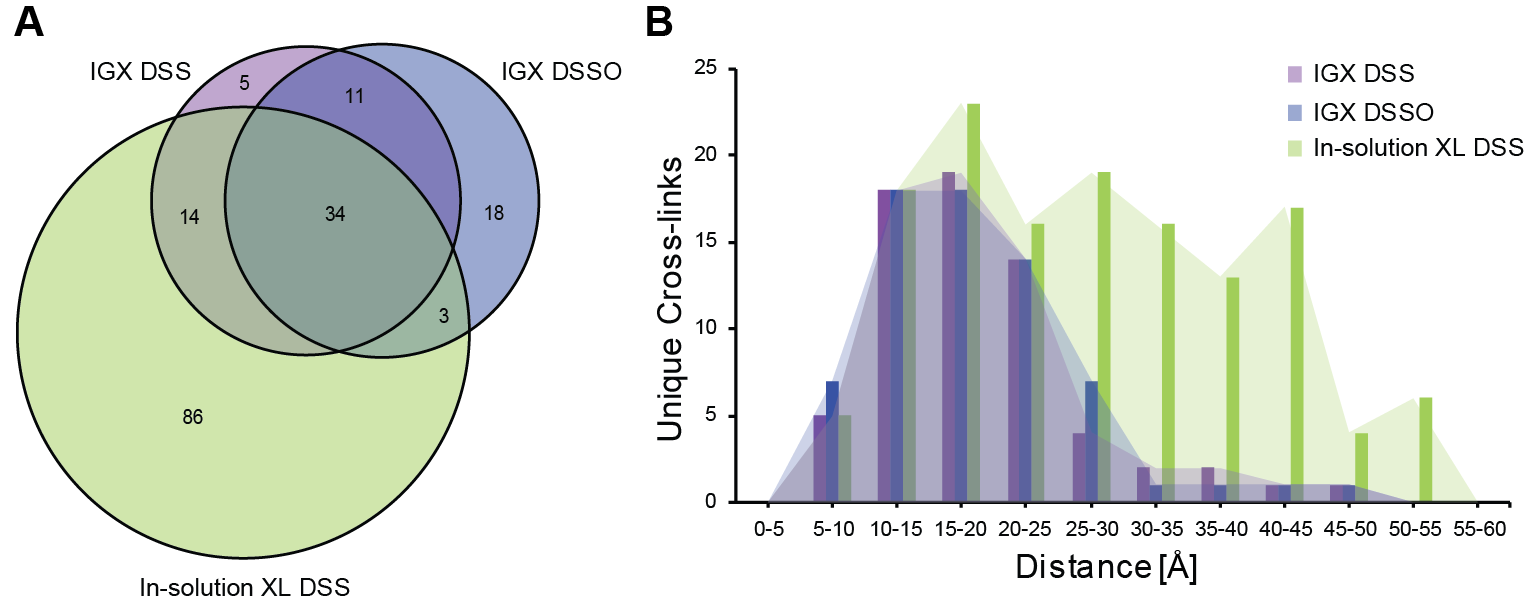
\includegraphics[]{Chapter.2/Figures/Figure3.png} 
\caption{\textbf{Comparison of IGX-MS and in-solution XL-MS of GroEL.} \textbf{A.} \emph{Escherichia coli} GroEL was subjected to in-solution XL-MS using 0.75 mM DSS. The resulting cross-links were compared to cross-links obtained by IGX-MS using DSS (1.5 mM) or DSSO (2 mM). The Venn diagram shows the overlap in the cross-links identified. \textbf{B.} Distribution of lysine C$\alpha$-C$\alpha$ distances of unique cross-links identified by IGX-MS (DSS or DSSO) or in-solution XL-MS plotted on the GroEL structure (PDB ID:1KP8).}
\label{fig:ch2_fig3}
\end{figure*}

\subsection*{IGX-MS facilitates the analysis of distinct co-occurring assemblies}
Proteins in cells or extracted from various biological sources can be part of multiple different complexes. Whether a protein is a free monomer or part of one or more protein complexes can substantially affect its structure. The identification of distinctive structural states of a protein by XL-MS in solution is often hampered, especially when the "free" monomer co-exist with the same protein being part of one or more complexes. For this reason, we investigated whether IGX-MS can exclusively obtain cross-links for proteins in a single configuration of the complex. As a first test-sample, we incubated GroEL with one of its known natural unfolded substrates, namely the bacteriophage T4 capsid protein (gp23, 56 kDa). Following incubation of GroEL with unfolded gp23, we analyzed this sample by BN-PAGE and observed three distinctive bands, corresponding to free GroEL and GroEL with one or two copies of gp23 bound (\textbf{\autoref{fig:ch2_app_fig4}A}). That GroEL can bind two substrate molecules (in the cis and trans ring) agrees with previously reported data \cite{van_Duijn_2006} and could be additionally confirmed by relative quantification of the subunits in the respective bands (\textbf{\autoref{fig:ch2_app_fig4}B}). In parallel cross-linking of each band, i.e., GroEL, GroEL:gp23 and GroEL:(gp23)2, with DSS, revealed interlinks between GroEL and gp23 exclusively in the middle and upper band whereby the primary inter-linked residues in GroEL were identified as K42, K122, and K272 (\textbf{Dataset EV2}). The site with most cross-links to gp23 was K272, located at the outer edge of the cavity (\textbf{\autoref{fig:ch2_app_fig4}C-D}). IGX-MS of each BN-PAGE bands enabled the identification of protein compositional specific distance restraints, which would have been impossible by in-solution XL-MS without additional experimental steps.\\
Next, we assessed the capabilities of IGX on a more complex sample and subjected 20 $\mu$g of purified bovine heart mitochondria (BHM), solubilized with digitonin, to BN-PAGE (\textbf{\autoref{fig:ch2_fig4}A}). It is well-known that BN-PAGE can separate and visualize the different complexes of the mitochondrial respiratory chain, including many of the co-occurring super-complexes \cite{Schagger_2000}. The band corresponding to the monomeric form of complex V (the well-studied ATP synthase, which can also be abundantly present in a V2 dimeric form), was excised and subjected to IGX-MS using DSS (\textbf{\autoref{fig:ch2_fig4}A}). The detected cross-links were plotted onto the 3D structure (PDB ID: 5ARA) and compared to cross-links detected in a previously published data set from our lab, by in-solution XL-MS \cite{Liu_2018} (\textbf{\autoref{fig:ch2_fig4}B}, \textbf{Dataset EV3}). Visualizing the detected IGX-MS- and in-solution XL-MS cross-linked regions revealed their high consistency, indicating that these membrane protein complexes largely retain their quarternary, tertiary, and secondary structures in the BN-PAGE gel. Similar to the previous in-solution XL-MS experiments, only solvent-accessible regions of complex V subunits (which in intact mitochondria are facing the matrix) were detected in the IGX data. Further, we found that ATP5IF, a known inhibitor of the ATPase, was associated with the monomeric ATP synthase (\textbf{\autoref{fig:ch2_fig4}C}). Detected cross-links from the inhibitor to ATP5F1E, ATP5F1D, ATP5F1C, and ATP5F1B agree with the previously reported binding interface of ATP5IF and the ATPase \cite{Gledhill_2007}. In-solution XL-MS resulted in a higher number of unique cross-links (248 vs. 53 for IGX). However, like for GroEL, the C$\alpha$-C$\alpha$ distance distribution revealed that many in-solution XL-MS cross-links are well above the 30 Å cut-off (149 unique cross-links). The IGX-MS cross-links are predominantly below this set cut-off (only two unique cross-links above), highlighting the accordance of the IGX-MS generated restrains with the previously published structure of monomeric ATPase (\textbf{\autoref{fig:ch2_fig4}D}, \textbf{Dataset EV3}). We argue that some of these over-length cross-links detected by in-solution XL-MS may originate from co-occurring dimeric complex V or other ATPase conformations induced upon binding of one (or several) of its many previously identified interactors \cite{Liu_2018, Ryl_2020, Schweppe_2017}. Additionally, IGX-MS generated cross-links exclusively describe the interaction of ATP5IF to monomeric ATP synthase. In contrast, in-solution XL-MS generated cross-links most-likely reflect distance restraints for different assembly states of ATP synthase (e.g., monomeric/dimeric ATP synthase with and without ATP5IF). To further showcase the ability of IGX-MS to generate assembly state-specific cross-links, bands corresponding to monomeric complex I (CI) and the super complex 1 (S1) were excised and subjected to IGX-MS using DSS (\textbf{\autoref{fig:ch2_app_fig5}A}). For both assembly states, a similar interaction network between the CI subunits was observed (\textbf{\autoref{fig:ch2_app_fig5}A}, \textbf{Dataset EV3}), revealing subunits that are in close proximity to each other in assembled CI (PDB ID: 5GUP). Cross-links detected for the super complex 1 (S1) revealed inter-complex links between\\

\begin{figure*}[hbt!]
\center
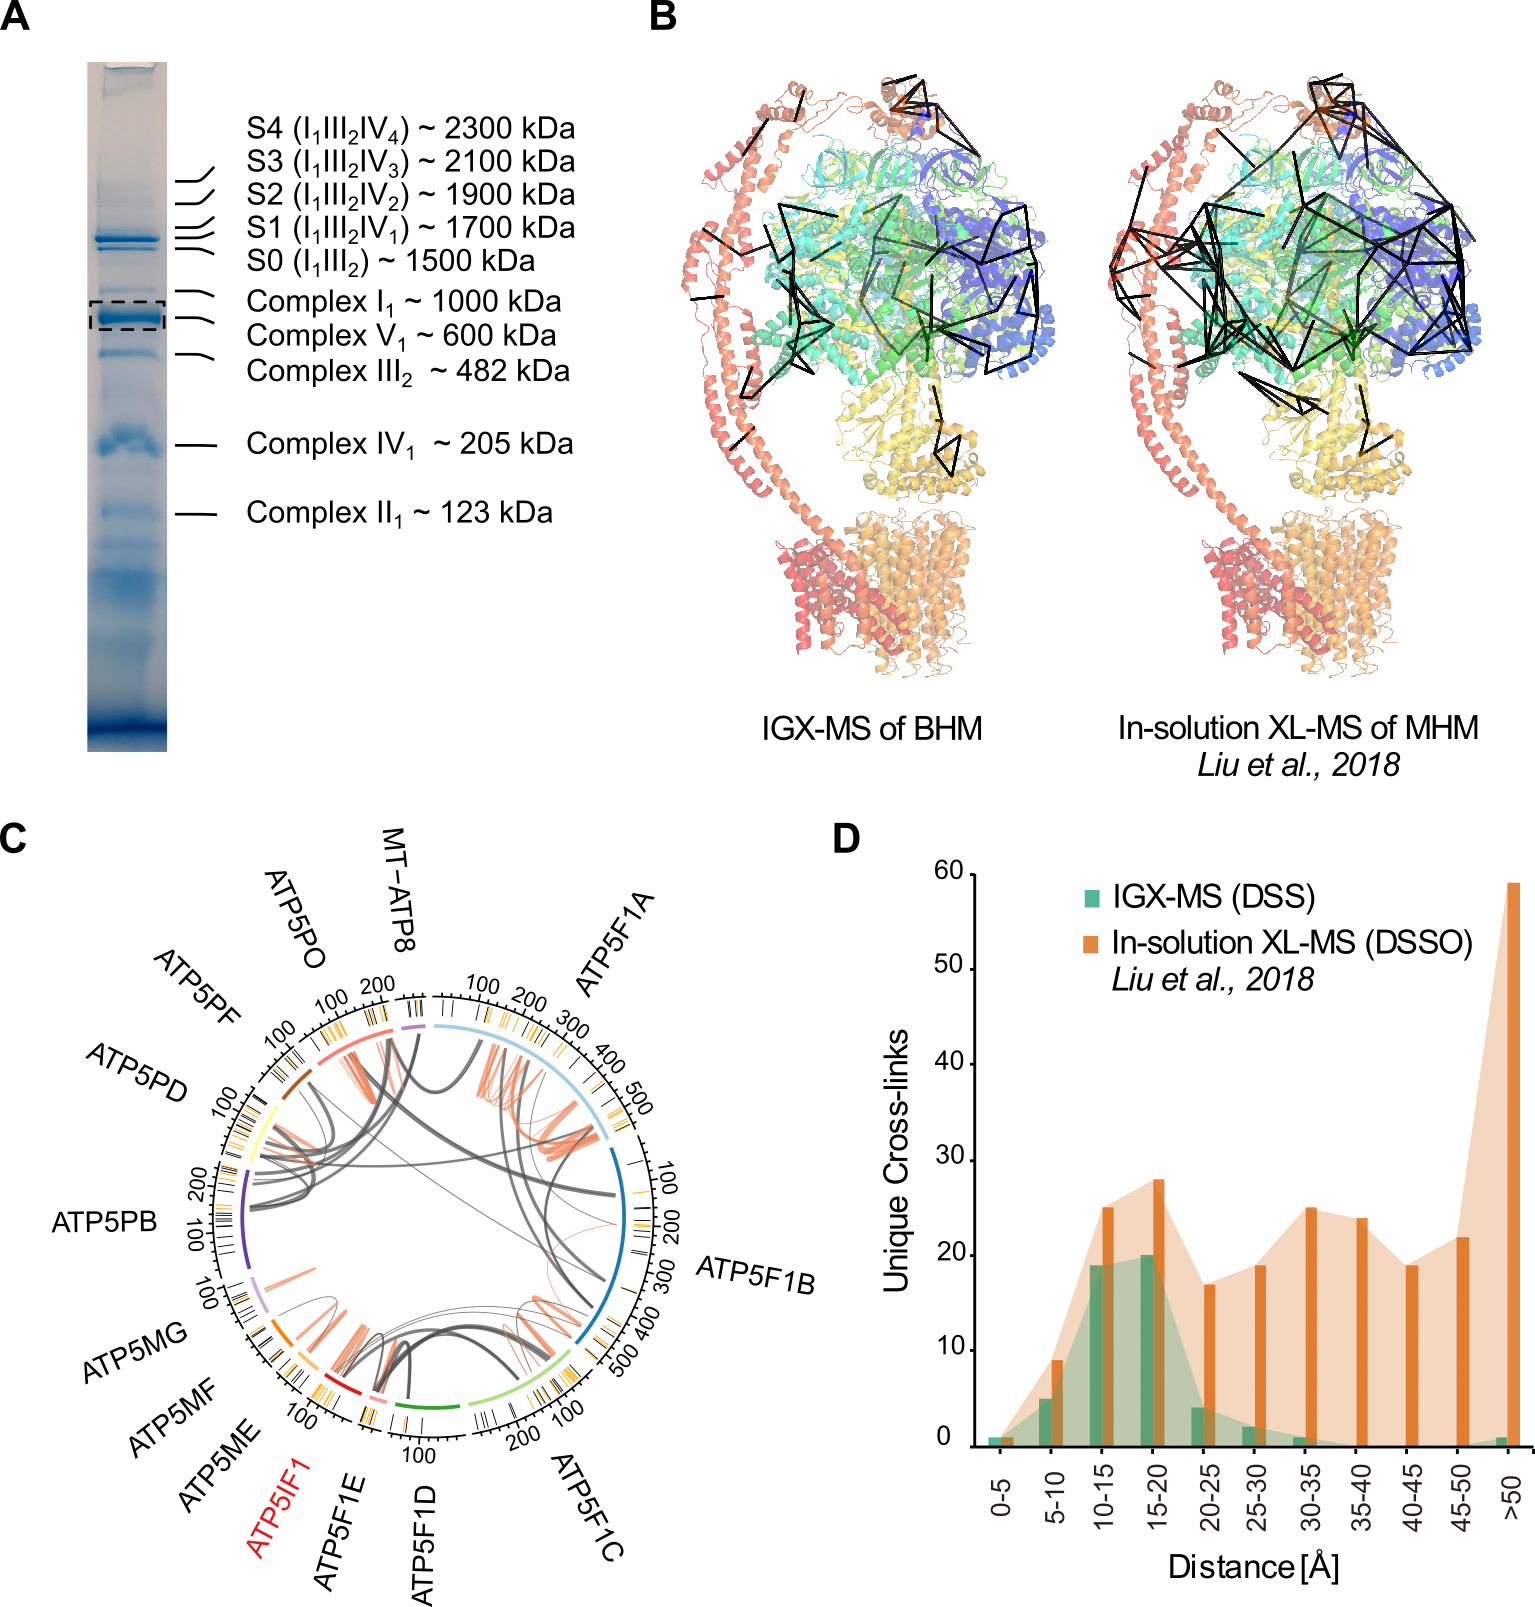
\includegraphics[]{Chapter.2/Figures/Figure4.png} 
\caption{\textbf{Selective cross-linking of the ATP synthase monomer from bovine heart mitochondria (BHM) by IGX-MS.} \textbf{A.} BN-PAGE of 20 $\mu$g solubilized BHM with several of the distinct complexes annotated. The dashed box indicates the monomeric ATP synthase (complex V) band subjected to IGX-MS. Annotation of protein bands was done following a previously published study \cite{Wittig_2010}. \textbf{B.} Unique cross-links < 30 Å identified by IGX-MS in this study (left) or by Liu \emph{et al} \cite{Liu_2018} using in-solution XL-MS plotted on the ATP synthase structure (PDB ID:5ARA). \textbf{C.} Circos plot of cross-linked ATP synthase subunits and the ATP synthase inhibitor (ATP5IF1) identified by IGX-MS. The position of the lysine residues is shown in the outer-ring, and cross-linked residues are colored dark orange. Orange lines represent intra-links while inter-links are colored dark gray. Thickness of the cross-link lines correlates to the number of detected cross-linked spectra matches (CSMs). \textbf{D.} Distribution of lysine C$\alpha$-C$\alpha$ distances of unique cross-links identified by IGX-MS or in-solution XL-MS \cite{Liu_2018} using DSS (1.5 mM) or DSSO (0.5 mM), respectively.}
\label{fig:ch2_fig4}
\end{figure*}
\clearpage

NDUFB4 (a subunit of complex I), UQCRC1, UQCRB (both subunits of complex III), COX7A1, and COX5B (both subunits of complex IV). This data agrees with the previously published structure \cite{Wu_2016}, which identified respective subunits in the interface regions of S1 (\textbf{\autoref{fig:ch2_app_fig5}A}, PDB ID: 5GUP). As reported for the ATP synthase, IGX-MS data for CI (monomeric and S1) closely resembles the previously reported in-solution XL-MS data \cite{Liu_2018} (\textbf{Dataset EV3}). Moreover, the targeted approach of IGX-MS allowed us to distinguish cross-links coming from monomeric CI or CI as part of S1, whereas in-solution XL-MS data represents a mixture of all the different assembly states (e.g., monomeric and S0-S4) (\textbf{\autoref{fig:ch2_fig4}A}, \textbf{\autoref{fig:ch2_app_fig5}B}).
In summary, comparing the IGX-MS and in-solution XL-MS cross-links for mitochondrial complex V, complex I and S1 highlights the capability of IGX-MS to generate sufficient, reliable and assembly-specific distance restraints.

\subsection*{Structural features of the complement proteins C5 and C6 and how these adapt when complexed into C5b6}
The terminal pathway of the complement system is mediated by sequentially interacting proteins (a.o. C5 to C9) that undergo various conformational changes in response to interactions with each other and the membrane environment \cite{Bajic_2015, Bayly-Jones_2017, Hadders_2012, Schatz-Jakobsen_2016}. In this process, membrane attack complex (MAC) is typically formed on the membrane of bacteria or pathogens, which leads to their elimination. Briefly, C6 binds to C5b, which originates from C5 by proteolytic cleavage. The resulting C5b6 complex binds C7, C8, and C9 sequentially, forming the C5b-9 complex. This complex is assembled onto the bacterial membrane and combines with polymerizing C9 molecules to create a lytic pore termed MAC \cite{Esser_1994}. Several structures of the different components of the terminal pathway have been explored by X-ray crystallography and electron microscopy (EM) \cite{Aleshin_2012, DiScipio_1988, DiScipio_1989, Fredslund_2008, Hadders_2012, Lovelace_2011, Menny_2018}. Especially well-resolved structures of monomeric C5, C6, and C5b6 contributed to understanding conformational changes that these proteins undergo in forming the C5b6 complex \cite{Aleshin_2012, Fredslund_2008, Hadders_2012}. We set out to investigate these different conformations by applying IGX-MS on monomeric C5, monomeric C6, and the hetero-dimeric C5b6 complex. Therefore, the BN-PAGE bands representing monomeric C5, monomeric C6, and C5b6 were subjected to IGX-MS (\textbf{\autoref{fig:ch2_app_fig6}A}). Cross-links obtained for both C5 and complexed C5b were in good agreement with the respective available structural models (PDB ID: 3CU7 and 4A5W) (\textbf{\autoref{fig:ch2_fig5}A,B}, \textbf{Dataset EV4}). In the C-terminal region of free C5, we detected some cross-links that exceed the distance restraint. This region is known to undergo significant structural rearrangements, as it adopts a more open conformation after conversion to C5b (\textbf{\autoref{fig:ch2_fig5}A}, \textbf{\autoref{fig:ch2_app_fig6}B}).

\begin{figure*}[b!]
\center
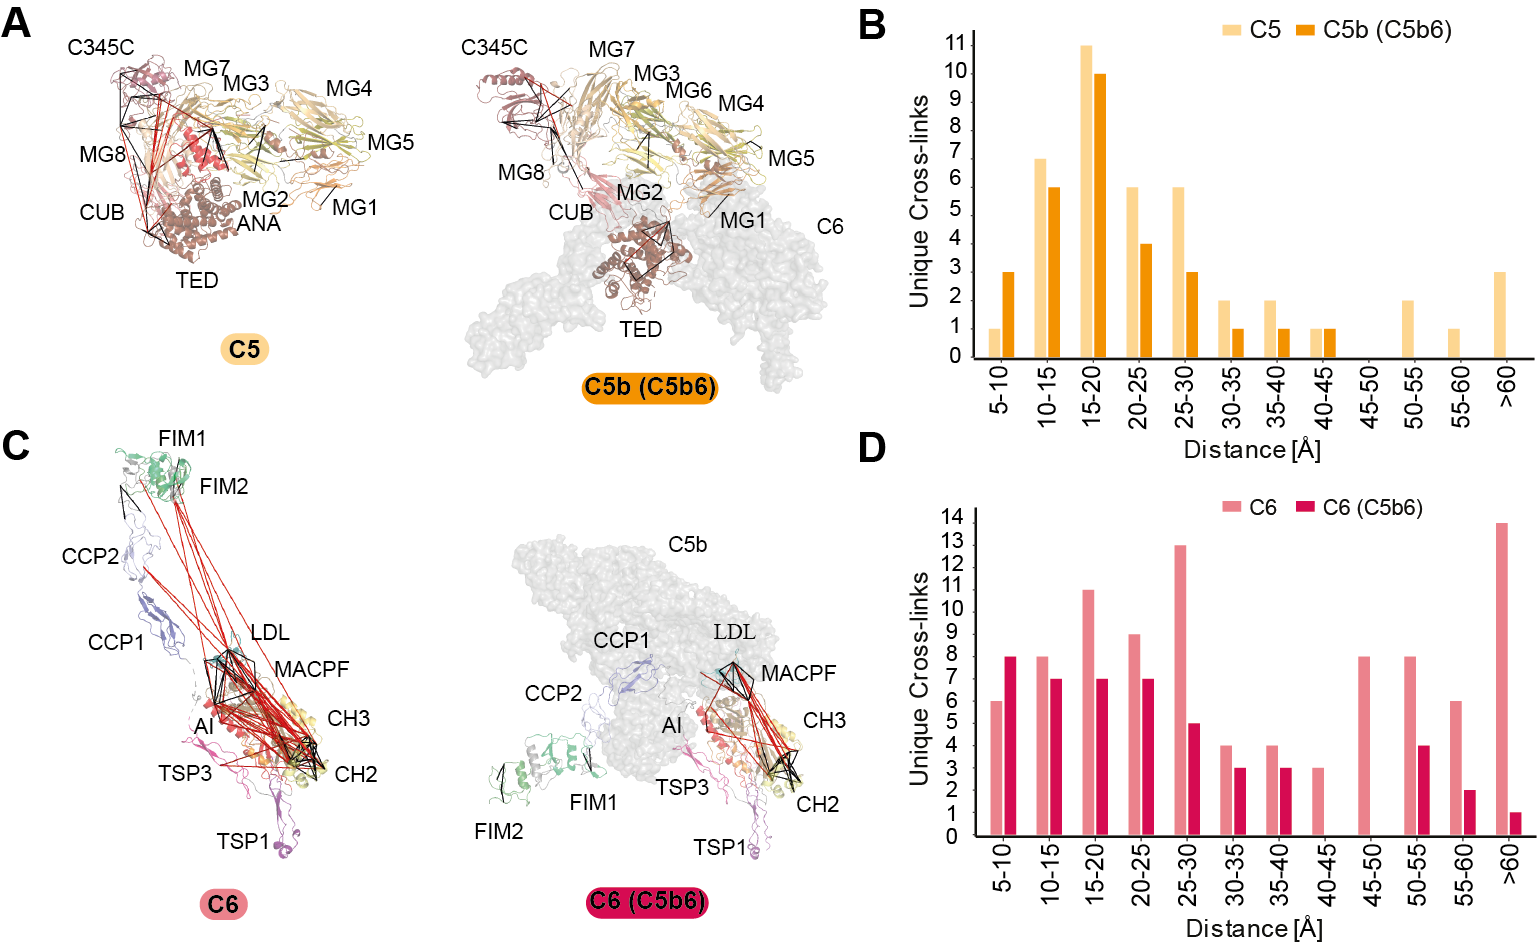
\includegraphics[]{Chapter.2/Figures/Figure5.png} 
\caption{\textbf{IGX-MS of the monomeric complement proteins C5 and C6, and the hetero-dimeric C5b6 complex.} \textbf{A.} Cross-links of monomeric C5 (left) and from C5b incorporated in the C5b6 complex (right) plotted on the respective available structural models (PDB ID: 3CU7 and 4A5W, respectively). The red lines indicate distances >30 Å. The different domains of C5 are indicated, and C6 within the C5b6 complex is shown in grey. \textbf{B.} Distribution of lysine C$\alpha$-C$\alpha$ distances of unique cross-links identified by IGX-MS in monomeric C5 (light orange) and C5b when part of the C5b6 complex (dark orange). \textbf{C.} Cross-links of monomeric C6 (left) and C6 incorporated in the C5b6 complex (right) plotted on the respective structural models (PDB ID: 3T5O and 4A5W, respectively). The red lines indicate distances >30 Å. The different domains of C6 are indicated, and C5b within the C5b6 complex is shown in grey. \textbf{D.} Distribution of lysine C$\alpha$-C$\alpha$ distances of unique cross-links identified by IGX-MS in monomeric C6 (light red) or C6 when incoprorated within the C5b6 complex.}
\label{fig:ch2_fig5}
\end{figure*}
\clearpage

Likewise, cross-links obtained for monomeric C6 and complexed C6 were plotted onto previously reported structural models (PDB ID: 3T5O and 4A5W) (\textbf{\autoref{fig:ch2_fig5}C}, \textbf{Dataset EV4}). Cross-links obtained for C6 when present in C5b6 were consistent with the previously published C5b6 structure (PDB ID: 4A5W). In contrast, cross-links obtained for monomeric C6 (PDB ID: 3T5O) did not substantiate the existing structural model and showed a noticeable bimodal distance distribution (\textbf{\autoref{fig:ch2_fig5}D}). Full-length C6 is composed of three thrombospondin (TSP) domains, a membrane attack complex/perforin (MACPF) domain, an LDL-receptor class A (LDL) domain, and an epidermal growth factor-like (EGF) domain. The EGF domain is followed by the C5b-binding domain composed of two complement control protein domains (CCP1 and CCP2) and two C-terminal factor I modules (FIM1 and FIM2), which are connected to the main body through a partially unresolved flexible linker (\textbf{\autoref{fig:ch2_fig5}C}). Interestingly, a high number of over-length cross-links (> 30 Å) in monomeric C6 were observed between the LDL domain and the MACPF, as well as within the MACPF domain itself. Cross-links exceeding the distance constraint within the MACPF are connecting the previously described autoinhibitory region (AI, residue 480-522) to two $\sim$50-residue helical clusters (CH1, residue 236-288; CH2 residue 363-416) (\textbf{\autoref{fig:ch2_fig5}C}, \textbf{\autoref{fig:ch2_app_fig6}C}) \cite{Hadders_2012}. Secondly, several over-length cross-links were observed between the FIM2 domain and the LDL and MACPF domain residues. These over-length cross-links are nearly exclusively detected for monomeric C6 and not for C6 when present in C5b6 (\textbf{\autoref{fig:ch2_fig5}C}, \textbf{\autoref{fig:ch2_app_fig6}C}).

\subsection*{Cross-link guided structural refinement of monomeric free C6}
Monomeric C6 displayed an intolerably high number of over-length cross-links suggesting that an alternative conformation of monomeric free C6 may (co-)exist. Based on identifying the lysine residues involved in these over-length cross-links, such an alternative structure would include re-positioning of the MACPF-, LDL- and the C5b-binding domains. We sought to define a structural model for monomeric C6 in two consecutive modeling steps. Our final refined model (\textbf{\autoref{fig:ch2_fig6}A}) retained the characteristic sequence-specific secondary structure elements and is only missing the flexible linker domain (residues 591-619), for which no confident distance restraints were available, likely due to the lack of lysine residues in this region. The missing linker comprises 28 amino acids, resulting in an 81 Å-gap in the IGX-MS driven model of C6 (\textbf{\autoref{fig:ch2_fig6}A} - black dots). Considering an average residue length of 3.4 - 4 Å, the length of this linker translates to 95.2 - 112 Å, which is sufficient to accommodate the produced gap \cite{Ainavarapu_2007}. When comparing the inter-domain rotation angles and domain centroid displacements between our model and the monomeric C6 X-ray structure (PDB ID: 3T5O), it becomes apparent that the main body (TSP1-1-TSP1-2-LDL-MACPF-EGF-TSP1-3) and the C5b-binding region (CCP1-CCP2-FIM1-FIM2) undergo a significant motion to each other (angle of 32 ° and displacement of 110.0 Å between TSP1-3 and FIM1 - \textbf{\autoref{fig:ch2_fig6}B}, \textbf{Table EV1}). On the other hand, the C5b-binding region moves almost like a single body with small inter-domain angles and displacements (largest angle of 2 ° and largest displacement of 1.1 Å). Within the main body, substantial domain reorientations can also be observed; in particular between EGF and TSP1-3 (angle of 83 ° and displacement of 16.7 Å), between TSP1-1 and TSP1-2 (angle of 42 ° and displacement of 19.7 Å), and between EGF and TSP1-3 (angle of 29 ° and displacement of 16.3 Å) (\textbf{\autoref{fig:ch2_fig6}B}, \textbf{Table EV1}). Further, when comparing the MACPF domain of the IGX-MS driven model to the previously reported structures of monomeric, complexed, and activated C6, noticeable intra-domain differences are obtained (\textbf{\autoref{fig:ch2_app_fig7}A-D}). Overall, the MACPF domain comprises a central four-stranded $\beta$-sheet, an AI region dominated by a linchpin helix, and three helical clusters (CH1-3) of which CH1 and CH2 unfold upon C6 activation (\textbf{\autoref{fig:ch2_app_fig7}A}). Closer examining the MACPF domain of the monomeric C6 X-ray structure (\textbf{\autoref{fig:ch2_app_fig7}B}) revealed a remarkable conformational resemblance with the MACPF domains of complexed C6 (\textbf{\autoref{fig:ch2_app_fig7}C}) and activated C6 (\textbf{\autoref{fig:ch2_app_fig7}D}). Interestingly, in our cross-linked driven structural model, we obtained a different conformational orientation of the regions within the MACPF domain (\textbf{\autoref{fig:ch2_app_fig7}A}). A clear re-positioning of the linchpin helix (part of the AI region), as well as the CH1 and CH2 cluster, can be delineated when compared to the MACPF of the X-ray structure (\textbf{\autoref{fig:ch2_app_fig7}E}). Here, the linchpin helix of the IGX-MS driven model (sand-colored structure) is tilted towards the central $\beta$-sheets and the helical clusters (CH1-3) (\textbf{\autoref{fig:ch2_app_fig7}F}). Additionally, the CH1 and CH2 domains are shown to be re-located, with the CH1 domain moved upwards, and the CH2 domain tilted towards the linchpin helix when compared to the MACPF domains of the previously reported monomeric, complexed and activated C6 structures (\textbf{\autoref{fig:ch2_app_fig7}F}). Conclusively, the structural rearrangements, guided by our IGX-MS data, result in a more closed conformation of the MACPF domain for free monomeric C6. Besides over-length cross-links within the MACPF domain, we detected eight cross-link restraints between the C5b-binding domain (specifically CCP2, FIM1, and FIM2) and LDL- and the MACPF-domain (specifically CH2) (\textbf{\autoref{fig:ch2_app_fig8}A}). The domains that are usually involved in the binding interface of C6 and C5b (CCP1 and CCP2 - see \textbf{\autoref{fig:ch2_fig5}C}) are in our model predicted to wrap around the MACPF domain, sharing an interaction interface with its CH2 and CH3 cluster (\textbf{\autoref{fig:ch2_fig6}A}, \textbf{\autoref{fig:ch2_app_fig8}B}). The FIM2 domain formes an interaction interface with residues of the TSP2, LDL, and MACPF domain, thereby locking the C5b-binding domain to the main body of C6 (\textbf{\autoref{fig:ch2_fig6}A-B}, \textbf{\autoref{fig:ch2_app_fig8}C}, \textbf{Dataset EV5}). This observation is in sharp contrast to the reported X-ray structure, in which the C5b-binding domain shows an "elongated" conformation, with no interaction interface between the mentioned domains (\textbf{\autoref{fig:ch2_fig6}B}). Further, we generated contact-maps to assess the overlap of cross-link data with the C6 X-ray structure and the IGX-MS driven model. The IGX-MS driven model provides new contact possibilities between the C5b-binding domain and the LDL-, and MACPF domain as well as within the MACPF domain (\textbf{\autoref{fig:ch2_fig6}C}), thereby significantly improving the overlap between the IGX and reported structural data (\textbf{\autoref{fig:ch2_fig6}D}, \textbf{Dataset EV4} and \textbf{Dataset EV6}). To validate the structural model for C6, we additionally performed an in-solution XL-MS experiment on purified C6. Firstly, the optimal cross-linker concentration was determined by incubating C6 with varying DSS concentrations (0-1.5 mM) (\textbf{\autoref{fig:ch2_app_fig9}A}). The optimization also revealed the formation of low amounts of dimeric C6 at all used crosslinking concentrations (\textbf{\autoref{fig:ch2_app_fig9}A}). Thus, an additional SDS-PAGE was performed following the in-solution cross-linking reaction (using 0.25 mM DSS)

\begin{figure*}[b!]
\center
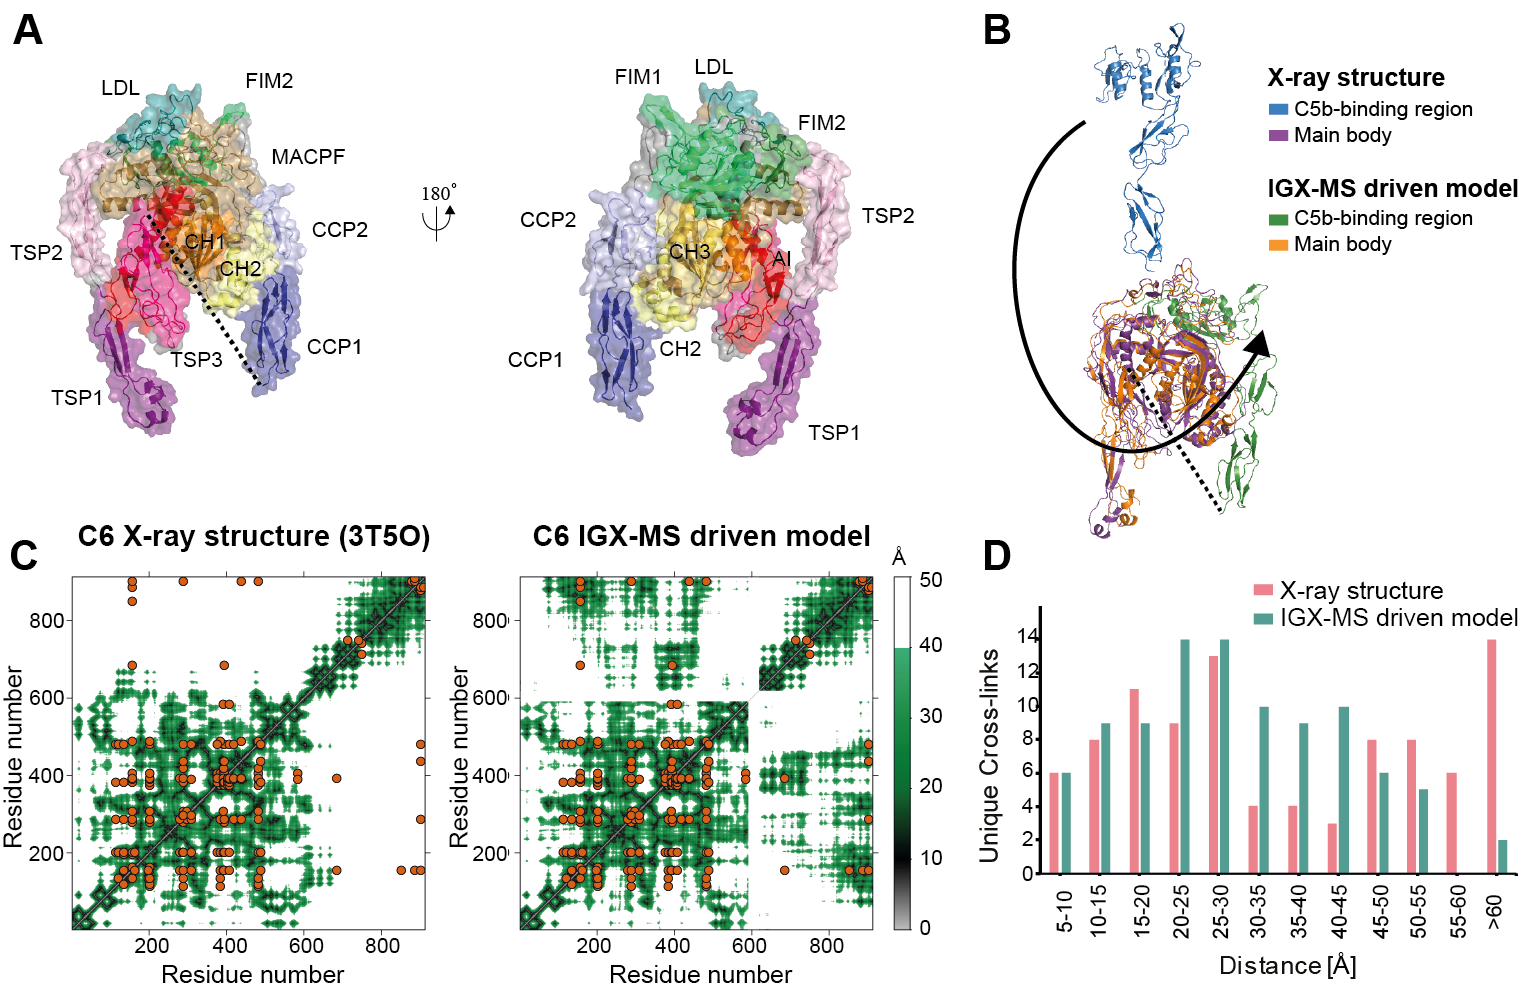
\includegraphics[]{Chapter.2/Figures/Figure6.png} 
\caption{\textbf{IGX-MS driven refined structural model of monomeric C6.} \textbf{A.} IGX-MS driven homology model of monomeric free C6 depicted in two different orientations. Black dots indicate the few missing amino acids (residue 591-619, spanning about 81 Å) covering the linker region between the main body and C5b-binding region. \textbf{B.} Superpositioning of C6 IGX-MS driven model (purple and green surface) and C6 X-ray structure (orange and blue surface; PDB ID: 3T5O). Black dots indicate the few missing amino acids (residue 591-619) covering the linker region between the main body and C5b-binding region. \textbf{C.} Contact maps with cross-linked residues (orange dots) of C6 X-ray structure (PDB ID: 3T5O, left panel) and IGX-MS driven C6 model (right panel). The colored density represents a contact relationship smaller than 40 Å of individual residues. White density represents a contact relationship bigger than 40 Å of individual residues. \textbf{D.} Distribution of lysine C$\alpha$-C$\alpha$ distances of unique cross-links identified by IGX-MS for monomeric C6 when plotted on the reported X-ray structure (pink bars, PDB ID: 3T5O) and the IGX-MS driven refined structural model (green bars).}
\label{fig:ch2_fig6}
\end{figure*}

to selectively detect crosslinks for monomeric C6. The in-solution generated cross-links were in agreement with the IGX-MS generated cross-links for monomeric C6, thereby suggesting a re-positioning of the MACPF-, LDL- and the C5b-binding domains (\textbf{\autoref{fig:ch2_app_fig9}B}). Finally, like for IGX-MS generated cross-links, the by in-solution XL-MS generated distance restraints for monomeric C6 are better satisfied for our cross-linked refined structural model than the X-ray structure (mean cross-link distance 26.2 Å vs. 41.7 Å - \textbf{\autoref{fig:ch2_app_fig9}C}).

\section{Discussion}
In-solution XL-MS has become a useful tool to study protein structures and protein-protein interactions \cite{Henry_2018, Koukos_2020, Liu_2014}. Even though the technology of in-solution XL-MS advanced substantially over the last decade, there are still quite a few challenges left. The current in-solution XL-MS method is time and labor demanding. Further, in-solution XL-MS requires a considerable amount of sample, which is necessary for optimizing the cross-linker concentration and the enrichment of cross-linked peptides. Also, in-solution co-occurring protein oligomers and distinct protein complexes within a sample can complicate the structural analysis. Unfortunately, current in-solution XL-MS workflows need further experimental steps to separate these protein complexes and potentially demand higher starting material amounts.\\
Here we introduce IGX-MS, an alternative approach that aims to tackle some of the challenges of in-solution XL-MS mentioned above. Firstly, we demonstrate the feasibility of cross-linking proteins in a BN-PAGE gel environment. We show that the efficiency of the in-gel cross-linking reaction is cross-linker- and also concentration-independent (DSS and DSSO work equally well). The latter makes the time- and sample consuming cross-linker concentration optimization obsolete. BN-PAGE combined with IGX-MS is very sensitive, requiring only a few micrograms of a protein sample to dissect and study different co-occurring protein complexes. These features reduce sample preparation time as no purification of a protein/ protein complex of interest is needed and enables the analysis of samples that are only available in minimal quantities (and therefore not susceptible to conventionally used purification methods for in-solution XL-MS). Another step, which can be omitted by using IGX-MS, is the samples's buffer exchange into a cross-link compatible buffer since it occurs already in the gel. The IGX-MS data presented here is hallmarked by high reproducibility, and to a large extent, the observed cross-links agree with those found by parallel in-solution cross-links. We find this as an important conclusion. It supports that proteins in the BN-PAGE gel maintain their native quarternary, tertiary, and secondary structures, as previously suggested \cite{Poetsch_2000, Schafer_2006, Wittig_2007}. Compared to in-solution XL-MS, IGX-MS shows a desired significant reduction of over-length cross-links when plotted on reported structures. A closer investigation of in-solution and in-gel cross-links revealed that IGX-MS generates protein state-specific cross-links with fewer undesired cross-linking products than in-solution XL-MS. This specificity is mainly achieved due to the option to precisely cross-link a specific oligomeric state or individual protein complex of interest. Compared to in-solution XL-MS, IGX-MS also has some caveats. Not all proteins and proteins assemblies enter a BN-PAGE gel easily, and some do not migrate as well-defined bands. Further, the resolving power of commercially available gels can provide a challenge in resolving distinct protein assemblies close in size. However, gels can be cast in-house, using gradients optimized for specific mass regions, potentially allowing a fast and easy adaption and modification suitable for specific sample/protein types.\\
Following proof of concept studies on samples, ranging from GroEL to mitochondrial respiratory chain complexes, we ultimately demonstrate that the distance restraints generated by IGX-MS can also be used to guide computational homology modeling and refine structural models. The reported structure of monomeric free C6 obtained by X-ray crystallography has been suggested to be in a partially activated and extended state \cite{Aleshin_2012}. This partial activation was attributed to crystal lattice contacts with neighboring C6 molecules mimicking C5b in the C5b6 hetero-dimer (\textbf{\autoref{fig:ch2_app_fig10}}). Our IGX-MS driven refined structural model suggests a more compact structural arrangement for monomeric C6. The linchpin helix of the AI region becomes tilted with an imaginary rotational center around one of the previously identified hinge regions \cite{Aleshin_2012} and more closely located to the central $\beta$-sheet as well as the helical clusters (CH1, CH2), which are known to unfold in the activated MACPF complex \cite{Menny_2018}. This arrangement indicates that the linchpin helix interacts with the CH1 domain as previously suggested \cite{Aleshin_2012} and also with the central four-stranded $\beta$-sheet and the CH2 domain. A closer position of the linchpin helix might hint at an auto-inhibitory function, to tightly control the unfolding of respective regions. Next, the C5b-binding domain can be found wrapped around the LDL- and MACPF domain, stabilizing the more compacted MACPF domain. Satisfyingly, the here presented IGX-MS-driven structural model agrees quite well with the overall shape of C6 as reported in early negative stain EM data \cite{DiScipio_1989}. We compared our data to previously published structures of complexed and activated C6 to obtain new insights into the dynamic activation process of C6. Upon binding of C6 to C5b, the C5b-binding domain is no longer wrapped around the LDL-and MACPF domain of C6, offering a binding interface for C5b. Simultaneously, the linchpin helix rotates around the hinge region to the left, and the CH1 domain moves downwards, bringing the EGF domain of the AI and the CH1 cluster in close proximity. Further, the CH2 cluster opens up by bending slightly to the right, resulting in a more open conformation of the MACPF domain, which culminates in the complete unfolding of CH1 and CH2 to elongated $\beta$-sheets in MAC (\textbf{\autoref{fig:ch2_app_fig7}A-E}). This initial unfolding of C6 provides an alternative conformational step in the terminal complement pathway, eventually pointing towards a new structural state of the C6 domains that is characteristic for its unbound state. Further, it would be interesting to investigate whether such a mechanism could also be true for C7, which shares a similar domain structure. Subsequently, we performed XL-MS of C6 in-solution. The observed cross-links were in very good agreement with the IGX-MS derived data, and thus also fitted well on our refined C6 structural model. The agreement between the BN-PAGE and in-solution data show that proteins with a large conformational space can retain their native structures in BN-PAGE (\textbf{\autoref{fig:ch2_app_fig9}A-C}). The in-solution XL-MS of C6 also confirmed some of the caveats of in-solution XL-MS we mentioned above, as in this case DSS concentration optimization revealed formation of small amounts of C6 dimer at all used DSS concentrations (\textbf{\autoref{fig:ch2_app_fig9}A}). Thus, to ensure that only cross-links coming from monomeric C6 were analyzed, we implemented another gel-based experimental step (SDS PAGE separation) for in-solution XL-MS of C6 to extract only cross-links for the C6 monomer.\\
The work presented here collectively describes a novel methodology termed IGX-MS, which allows the efficient, sensitive, and reproducible generation of specific structural distance restraints. The methodology described here should not be regarded as replacement for in-solution XL-MS, but rather as a convenient, alternative approach. IGX-MS can best be used on proteins and protein complexes that can be well-separated in a BN-PAGE gel and this is not the case for all proteins. But when amendable to BN-PAGE, IGX-MS provides the ability to distinctively analyze co-occurring protein oligomers in purified systems, even when originating from more complex samples, such as solubilized mitochondria.

\section{Material and Methods}
\subsection*{Materials}
Chemicals and reagents were purchased from Sigma Aldrich (Steinheim, Germany) unless otherwise stated. Acetonitrile (ACN) was purchased from Biosolve (Valkenswaard, The Nederlands). Sequencing grade trypsin was obtained from Promega (Madison, WI). NativePAGE 3-12 \% Bis-Tris protein gels, NativePAGE Sample Buffer, NativePAGE Running Buffer, NativePAGE Cathode Additive, and NativeMark were purchased from Invitrogen (California, USA). Criterion XT Bis-Tris Precast Gels (4-12 \%), XT MOPS Running Buffer, and sample buffer were purchased from BioRad (California, USA). DSSO was produced in-house according to a previous protocol \cite{Kao_2011}. Oasis HLB 96-well $\mu$Elution Plates were purchased from Waters (Massachusetts, USA). GroEL and the major capsid protein gp23 were expressed and purified as previously described. \cite{Quaite-Randall_2000, van_Duijn_2005, van_Duijn_2006} Complement components C5, C6, and C5b6 were purchased from CompTech (Texas, USA). The fresh bovine heart was obtained from a slaughterhouse.

\subsection*{Separation of proteins using Blue native PAGE (BN-PAGE)}
Blue native page analysis was performed according to the manufacturer's protocol and recently published protocols \cite{Wittig_2006}. Briefly, proteins were mixed with NativePAGE sample buffer (1x final concentration), and subsequently, 5-20 $\mu$g of protein sample was loaded onto a Bis-Tris gel (3-12 \%). Electrophoresis was started with a dark blue cathode buffer (1x NativePAGE cathode additive) for 30 min at 80 V before the dark blue buffer was changed to light blue cathode buffer (0.1x NativePAGE cathode additive). After the change of buffer, the voltage was increased to 120-140 V for additional 2-4 hours. Readily run gels were briefly rinsed with ddH2O before gel bands of interest were excised and further cut into smaller pieces under a laminar flow hood. Excised protein bands were stored in Eppendorf tubes for subsequent cross-linking experiments.

\subsection*{Verification of in-gel cross-linking (IGX) by SDS-PAGE}
Purified GroEL (10 $\mu$g) in Tris buffer (50 mM Tris-HCL, pH 7.7, 1 mM EDTA, 1 mM DTT, 10\% glycerol) was analyzed using BN-PAGE as described above. Next, excised gel bands were incubated in 50 $\mu$L PBS with or without 1.5 mM DSS for 30 min at room temperature (RT). Then the cross-linking reaction was quenched by addition of Tris to a final concentration of 50 mM for 30 min at RT. Next, the supernatant was removed from the gel pieces, and proteins were extracted in 200 $\mu$L extraction buffer (50 mM Tris, pH 7.9, 1 mM dithiothreitol (DTT), 150 mM NaCl, 0.1\% SDS) overnight at RT. The gel pieces were separated by centrifugation at 14,000 x g for 2 min, and the supernatant dried to 20 $\mu$L. The samples were heated to 95 °C for 5 min with 50 mM DTT and sample buffer before loaded onto SDS-PAGE (4-12\%). The gel was prepared according to the manufacturer's protocol using MOPS running buffer. After the SDS-PAGE separation finished, the gel was briefly washed with ddH2O and subjected to Coomassie brilliant blue staining solution for approximately one hour. Stained SDS gels were de-stained in ddH2O, overnight and shaking at RT.

\subsection*{DSS and DSSO concentration range experiments with GroEL}
BN-PAGE followed by IGX of purified GroEL was performed as described before. Excised gel pieces were incubated with an increasing concentration of DSS and DSSO (0.5, 1, 1.5, 2, and 5 mM) to determine the effect of different cross-linker concentrations. Cross-linking experiments were performed in triplicates. After quenching of cross-linking reactions, the supernatant was removed, and gel pieces were briefly washed using ddH2O and subsequently subjected to standard in-gel digestion \cite{Shevchenko_2006}. Briefly, gel pieces containing cross-linked proteins were washed, reduced by incubation in reduction buffer (50 mM ammonium bicarbonate (AmBic), 6.5 mM DTT, pH 8.5) for one hour at RT. The reduction buffer was removed, and gel pieces were dehydrated using 100 \% ACN. Next, dehydrated gel pieces were subjected to alkylation buffer (50 mM AmBic, 54 mM iodoacetamide (IAA), pH 8.5) for 30 min at RT in the dark. The alkylation buffer was removed, and gel pieces were dehydrated using 100 \% ACN. For digestion of cross-linked proteins, dehydrated gel pieces were covered with digestion buffer (3ng/$\mu$L Trypsin in 50 mM AmBic, pH 8.5) and pre-incubated for a minimum 30 min on ice. Next, excess of digestion buffer was removed, and an equivalent volume of AmBic buffer (50 mM AmBic, pH 8.5) was added to cover the gel pieces, before incubating at 37 °C overnight. Next, the supernatant containing digested peptides was collected, and gel pieces were once again dehydrated using 100 \% ACN for 15 min at RT. Resulted supernatant was collected and combined with the previous supernatant. Finally, the samples were completely dried and stored at -80 °C until MS analysis. For MS analysis, cross-linked peptides were resuspended in MS buffer (10 \% FA in water) and analyzed as described below.

\subsection*{LC-MS analysis}
Data for IGX-MS samples was acquired using an UHPLC 1290 system (Agilent Technologies, Santa Clara, CA) coupled on-line to an Orbitrap Fusion or Orbitrap Fusion Lumos mass spectrometer (Thermo Scientific, San Jose, CA). Firstly, peptides were trapped using a 100-$\mu$m inner diameter 2-cm trap column (packed in-house with ReproSil-Pur C18-AQ, 3$\mu$m) prior to separation on an analytical column (50 cm of length, 75 $\mu$M inner diameter; packed in-house with Poroshell 120 EC-C18, 2.7 $\mu$m). Trapping of peptides was performed for 5 min in solvent A (0.1 \% FA in water) at a flow rate of 0.005 mL/min. DSS cross-linked peptides were subsequently separated as follows: 0-13 \% solvent B (0.1 \% FA in 80 \% v/v ACN) in 10 sec, 13-44 \% in 40 min, 44-100 \% in 3 min and finally 100 \% for 2 min. DSSO cross-linked samples were separated using the following gradient: 0-10 \% solvent B in 10 sec, 10-40 \% in 40 min, 40-100 \% in 3 min, and finally 100 \% for 2 min. For each of the gradients, the flow was passively split to approximately 200 nL/min. Mass spectrometers were operated in a data-dependent mode (DDA). For DSS cross-linked peptides, full scan MS spectra from 350-1500 Th were acquired in the Orbitrap at a resolution of 60,000 with the AGC target set to 1 x 106 and maximum injection time of 20 ms. For measurements on the Orbitrap Fusion, in-source fragmentation was turned on and set to 15 eV. Cycle time for MS2 fragmentation scans was set to 3 s. Only peptides with charged states 3-8 were fragmented, and dynamic exclusion properties were set to n = 1, for a duration of 20 ms. Fragmentation was performed using in a stepped HCD collision energy mode (31.5, 35, 38.5 \%) in the ion trap and acquired in the Orbitrap at a resolution of 30,000 after accumulating a target value of 1 x 105 with an isolation window of 1.4 Th and maximum injection time of 120 ms. For the acquisition of DSSO cross-linked peptides, full scan MS spectra from 310-1600 Th were acquired in the Orbitrap at a resolution of 120,000 with the AGC target set to 5 x 105 and maximum injection time of 50 ms. For the identification of DSSO signature peaks, peptides were fragmented using a fixed CID collision energy (30 \%) and MS2 scan was performed at in the Orbitrap at a resolution of 30,000 after accumulating a target value of 5 x 104 ions using an isolation window of 1.6 Th and maximum injection time of 54 ms. For sequencing selected signature peaks, selected ions were fragmented using a fixed HCD collision energy (30 \%) in the ion trap MS3, with the AGC target set to 1 x 104 and maximum injection time of 120 ms.
\raggedbottom
\subsection*{In-solution XL-MS of GroEL}
Purified GroEL (10$\mu$g) was cross-linked using 0-2 mM DSS for 30 min at RT, followed by quenching using a final concentration of 50 mM Tris. Cross-linked samples were analyzed by SDS-PAGE to determine an optimal cross-linker to protein ratio. The optimal DSS concentration (0.75 mM, \textbf{\autoref{fig:ch2_app_fig3}A}) was used for cross-linking of 20 $\mu$g GroEL (1mg/mL) in triplicates. After quenching of the reactions, protein precipitation was performed by adding three times 50 $\mu$L cold acetone and subsequent incubation at -20 °C overnight. Precipitated samples were centrifuged at 12,000 x g for 20 min. After careful removal of the supernatant, the remaining pellet was air-dried until no acetone solution was visible anymore. Pellets were resuspended in 50 $\mu$l ABC with 0.33 $\mu$g trypsin (1:60) and incubated with shaking for 4 h at 37 °C. The solubilized pellets were reduced by 5 mM TCEP for 5 min at 95 °C followed by alkylation with 30 mM CAA for 30 min at 37 °C. Digestion was performed overnight by 0.4 $\mu$g trypsin (1:50) at 37 °C. The samples were acidified with TFA before desalting using Oasis HLB plate. Finally, the eluent was dried completely and solubilized in 10 \% FA before MS-analysis.

\subsection*{Analysis of GroEL bound to unfolded gp23}
The major capsid protein gp23 was unfolded in 8 M urea for one hour at RT. Unfolded gp23 (11.4 $\mu$M) was incubated with GroEL (0.8 $\mu$M) in Tris buffer with ADP (50 mM Tris, pH 7.5, 50 mM KCl, MgCl2, 1 mM ADP) 10 min at RT. The samples were then subjected to BN-PAGE, as previously described. IGX-MS were performed on the three occurring bands, as described earlier, using 1.5 mM DSS.

\subsection*{Data analysis of GroEL cross-links}
Raw files obtained from IGX-MS of GroEL were analyzed with the Proteome Discoverer (PD) software suite version 2.3 (Thermo Fisher Scientific) with the incorporated XLinkX node for analysis of cross-linked peptides. For DSS data, the non-cleavable cross-link search option was used, while DSSO data was searched by the MS2/MS3 option. A FASTA file containing the GroEL sequence was used for the XlinkX search. For the samples of GroEL complexed with gp23, the FASTA file was supplemented with the sequences of GroEL and gp23. Raw files were searched with the precursor mass tolerance set to 10 ppm, the maximum FDR rate set to 1 \% and $\Delta$ XlinkX score $\geq$ 40. Carbamidomethyl was set as fixed modification and oxidation (M) and acetylation (protein N-term) as variable modifications. The obtained cross-links were plotted onto the GroEL structure (PDB ID:1KP8) to extract the C$\alpha$-C$\alpha$ distances using a python script for PyMol. For further cross-link analysis, both intra-chain and inter-chain combinations to neighboring subunits were considered. In the distance histograms, only the shortest combination is represented if several possible combinations existed. When plotted on the structure, several combinations are shown if they are below 30 Å. Cross-link sequence overviews were generated using xiNET \cite{Combe_2015}. Data obtained from IGX-MS of GroEL bound to gp23 was searched in MaxQuant (version 1.6.10.0) to obtain iBAQ (intensity-Based Absolute Quantification) values. Trypsin was set as a digestion enzyme with two allowed missed cleavages. Carbamidomethyl was set as fixed modification and oxidation (M) and acetylation (protein N-term) as variable modifications. The FASTA file used for the search contained sequences of GroEL and gp23.

\subsection*{Isolation and purification of bovine heart mitochondria (BHM)}
The bovine heart was freshly obtained from a slaughterhouse, kept on ice for 1 h and immediately used for mitochondria isolation. All procedures were performed within a cold room and/or maintaining the material and solutions on ice. The heart (ca. 600 g) was cut into smaller pieces while removing excess of fat and connective tissue. The pieces of cardiac muscle tissue were homogenized in 4 ml/g tissue of ice-cold isolation buffer (250 mM sucrose, 10 mM Tris/HCl pH 7.4, 0.5 mM EDTA and 2 mM phenyl-methane-sulfonyl fluoride) using a blender at low speed for 5 s and at high speed for 1 min. The pH of the homogenate was measured and corrected to 7.4 with 2 M Tris (unadjusted). After a 15 min stirring, the homogenate was centrifuged at 400 x g (20 min; 4°C). The supernatants were filtered through 8 layers of gauze and centrifuged at 7,000 x g (30 min; 4°C). The resulting mitochondria-enriched pellets were resuspended in isolation buffer and again homogenized this time by applying 10 strokes using a Potter-Elvehjem homogenizer. The mitochondrial homogenates were centrifuged at 10,000 x g (20 min; 4°C) and the resulting pellets (crude mitochondria) were resuspended in isolation buffer supplemented with protease inhibitor cocktail (SIGMAFAST™). Protein concentration was determined by the DC protein assay (Bio-Rad). Aliquots were shock-frozen in liquid nitrogen and stored at -80°C. In order to increase the purity of the preparation, crude mitochondria (4 x 15 ml aliquots; ca. 60 mg prot/ml) were thawed on ice, diluted (1:4) with ice-cold washing buffer (250 mM sucrose, 20 mM Tris/HCl pH 7.4, 1 mM EDTA) and centrifuged at 1,000 x g (10 min; 4°C). The supernatants were recovered and centrifuged at 40,000 x g (20 min; 4°C) and each resulting pellet (clean mitochondria) was resuspended in 2 ml washing buffer. Afterward, mitochondria were loaded onto a two-layer sucrose gradient (1 M/1.5 M) and centrifuged at 60,000 x g (20 min; 4°C). The fractions accumulated at the interphase (pure mitochondria) were carefully recovered and pooled into one tube. After resuspension in 20 ml ice-cold washing buffer, pure mitochondria were centrifuged at 10,000 x g (20 min; 4°C) and finally resuspended in 5 ml ice-cold washing buffer supplemented with protease inhibitor cocktail (SIGMAFAST™). Protein concentration was determined as above described and the aliquots of pure mitochondria were shock-frozen in liquid nitrogen and stored at -80 °C.

\subsection*{IGX-MS and data analysis of ATP synthase isolated from purified BHM}
Purified bovine heart mitochondria were solubilized with digitonin (9 g/g protein) on ice for 30 min. Subsequently, 20 $\mu$g of solubilized mitochondria was analyzed using BN-PAGE. Afterward, a band corresponding to the ATP synthase was excised, and IGX-MS was applied as described above using 1.5 mM DSS.Triplicates were measured, and individual raw files (corresponding to a specific gel band) were searched in MaxQuant (Cox and Mann, 2008) against the \emph{Bos Taurus} proteome (2019-08, downloaded from Uniprot) with a PSM FDR of 1 \%. Trypsin was set as a digestion enzyme with two allowed missed cleavages. Carbamidomethyl was set as fixed modification and oxidation (M) and acetylation (protein N-term) as variable modifications. Proteins identified for each raw.file were subsequently used to generate a "reduced" fasta file for the cross-link search in PD using the XlinkX node using previously described settings. Identified cross-links corresponding to the ATP synthase, Complex I and S1 complex (I-III3-IV) were subsequently extracted and plotted onto the previously published structure (PDB ID: 5ARA, 5GUP). Resulting C$\alpha$-C$\alpha$ distances were compared to previously published in-solution data for cross-linked mouse heart mitochondria \cite{Liu_2018}. An overview of cross-linked subunits for mentioned proteins was generated using the "circlize" package for R \cite{Gu_2014}.

\subsection*{IGX-MS and data analysis of complement proteins}
Complement components C5 (5 $\mu$g), C6 (5 $\mu$g), and C5b6 (10 $\mu$g) were subjected to BN-PAGE followed by IGX-MS as previously described using 1.5 mM DSS. Experiments were done in triplicates. The resulting raw files from the MS-analysis were searched in MaxQuant (version 1.6.10.0) to generate libraries for the C5, C6, and C5b6 bands. The data was searched against the reviewed Homo Sapiens Uniprot database (2019-08, downloaded from UniProt). Trypsin was set as a digestion enzyme with two allowed missed cleavages. Carbamidomethyl was set as fixed modification and oxidation (M) and acetylation (protein N-term) as variable modifications. The data was then searched using PD, as described earlier. Mannosylation of tryptophan residues was added as a variable modification, and MaxQuant generated libraries used in the XLinkX search. Only cross-links observed in two out of the three replicates were included for further analysis. The cross-links were plotted onto the respective structures using PyMol to obtain C$\alpha$-C$\alpha$ distances. Cross-link sequence overviews were generated using xiNET \cite{Combe_2015}.

\subsection*{Modeling of an alternative structure of free complement C6} Cross-links derived for free C6, together with additional structural constraints derived from Uniprot (disulfide-bond information, secondary structure elements; Uniprot Accession: P13671) were used to predict an alternative structural model. Briefly, the modeling process was divided into two consecutive steps. First, an I-Tasser homology model of C6 based on the previously published structure (PDB ID: 3T5O) was generated to resolve missing residues \cite{Yang_2015}. Next, a flexible linker region (residue 591-619) and the C5b-binding domain (residues 620-913) were removed from the generated C6 model. Subsequently, regions with a high density of cross-linked residues were removed from the shortened C6 structure, producing a "core-template" for comparative modeling using Modeller 9.24 \cite{Webb_2016}. Excised regions were provided as additional templates (Table EV2) to support the modeling process together with the cross-linking restraints (mean=17 Å, stdev=2) obtained for individual residues (1-590) as well as the secondary structure information which was obtained from Uniprot (Uniprot ID: P13671). In total, 20 cross-linked guided models for free C6 were generated, each first optimized with the variable target function method (VTFM) and afterwards refined using molecular dynamics (MD) optimization (Sali and Blundell, 1993). For each model, a DOPE score and a GA341 score was calculated to further validate the quality of produced models \cite{John_2003, Melo_2002, Shen_2006}. Additionally, contact maps for each one of the 20 models were generated, and a CM score \cite{Schweppe_2016} was calculated, indicating the overlap of the cross-linking data with the respective contact maps using the XLmap package in R \cite{Schweppe_2016} (Dataset EV7). The model satisfying both scores the best (DOPE and CM score) was chosen for the second modeling process, to generate a full-length model of C6 using detected cross-links between C6 (residues 1-590) and the C5b-binding domain (residues 620-913). The structural assembly of both was achieved by predicting an interaction interface by DisVis \cite{van_Zundert_2015} using respective cross-links and solvent-accessible residues as input parameters. Solvent accessible residues were identified using the standalone program Naccess (© S. Hubbard and J. Thornton 1992-6). Residues with relative solvent accessibility $\geq$ 40 \% were used as solvent-accessible residues. Finally, information-driven docking with HADDOCK \cite{Karaca_2011, van_Zundert_2016} with the validated cross-links and the identified active residues was performed, resulting in four distinct clusters. A file (.json) containing all parameters set for the protein docking was deposited to the ProteomeXchange partner PRIDE database (for details, see "Data availability" section). The structure showing the best agreement with the distance restraints used for the docking process and the best Haddock score was chosen as final model (Dataset EV8). Additionally, residues participating in a binding interface between the C6 (residues 1-590) and the C5b-binding domain were predicted using the Prodigy webserver (Dataset EV5). For final model validation, all IGX-MS derived cross-links obtained for C6 were plotted onto the model, and distances for respective links were compared to the Xray structure of C6 (PDB ID 3T5O) (Dataset EV6).

\subsection*{Characterization of inter-domain rotation angles}
From the comparison of our IGX-MS driven model with the crystal structure of C6 in isolation (PDB 3T5O), inter-domain rotation angles and centroid displacements were determined by sequentially superposing the domains (with indicated boundaries) of the crystal structure of C6 onto the corresponding domains of our model, using the program Superpose (Krissinel and Henrick, 2004), part of the CCP4 suite \cite{Winn_2011}. Superposition was based on C$\alpha$ atoms of indicated domains (Table EV1). To further compare the protein conformations, a distance map was generated using the Bio3D package for R \cite{Grant_2006}. For this, coordinates of superimposed MACPF domains (residue 155-501) extracted from the crystal structure, and our model were provided as input (\textbf{\autoref{fig:ch2_app_fig7}E}).

\subsection*{In-Solution XL-MS of C6}
Purified C6 (5$\mu$g, 0.33 mg/ml) was cross-linked using 0-1.5 mM DSS for 30 min at RT, followed by quenching using a final concentration of 50 mM Tris. Cross-linked samples were analyzed by SDS-PAGE to determine an optimal cross-linker to protein ratio. Lower DSS concentrations down to 10 $\mu$M were also tested. The optimal DSS concentration (0.25 mM, \textbf{\autoref{fig:ch2_app_fig9}}) was used for cross-linking of 20 $\mu$g C6 (0.33 mg/mL) in triplicates. After quenching the reactions, 5 $\mu$g was separated by SDS-PAGE, and the monomeric band was subjected to in-gel digest before XL-MS/MS analysis. Raw files were analyzed as previously described for IGX-MS of complement proteins using MaxQuant and the XlinkX node of PD using previously described settings. Identified cross-links were plotted onto the previously published crystal structure (Dataset EV4) and our IGX-MS driven model (Dataset EV6).

\subsection*{Data availability}
The mass spectrometry data from this publication have been deposited to the ProteomeXchange partner PRIDE database \cite{Vizcaino_2016} and assigned to the identifier PXD020014. EV Datasets and tables are available online with the original manuscript (Supporting Information).

\subsection*{Acknowledgments}
All authors acknowledge support from the Netherlands Organization for Scientific Research (NWO) funding the Netherlands Proteomics Centre through the X-omics Road Map program (project 184.034.019) and the EU Horizon 2020 program INFRAIA project Epic-XS (Project 823839). MVL thanks Independent Research Fund Denmark (project 9036-00007B). 

\subsection*{Author contributions}
JFH and AJRH conceptualized the study. JFH and MVL designed the methodology, performed experiments, and analyzed the data. ACO and SA provided the mitochondrial samples. MFP performed the characterization of inter-domain rotation angles. JFH and MVL wrote the original draft. JFH, MVL, MFB, ACO, SA, VF, AJRH carefully revised and edited the manuscript before submission. MVL and AJRH acquired funding and resources. AJRH supervised the project.

\subsection*{Conflict of interest}
The authors do not declare any conflict of interest.

\clearpage
\begin{subappendices}
    \counterwithin{figure}{section}
    \section{Supplementary Material}

    \begin{figure*}[hbt!]
        \center
        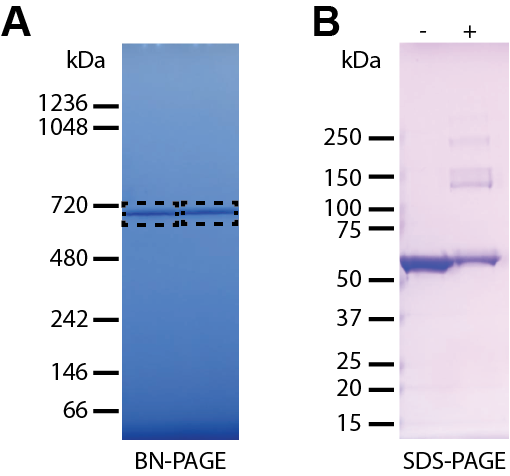
\includegraphics[]{Chapter.2/Figures/SI_Figure1.png} 
        \caption{\textbf{Combining BN-PAGE with IGX-MS.} \textbf{A.} BN-PAGE of E. Coli (10 $\mu$g). Respective bands (dashed boxes) were excised and incubated with or without the cross-linker DSS (1.5 mM). \textbf{B.} SDS-PAGE of GroEL, extracted from respective gel band (see A). The non-cross-linked control (-) showed only a band at 57 kDa of the GroEL subunit, whereas the DSS-cross-linked sample (+) reveals several bands at higher Mw.}
        \label{fig:ch2_app_fig1}
    \end{figure*}

    \vspace{1cm}

    \begin{figure*}[hbt!]
        \center
        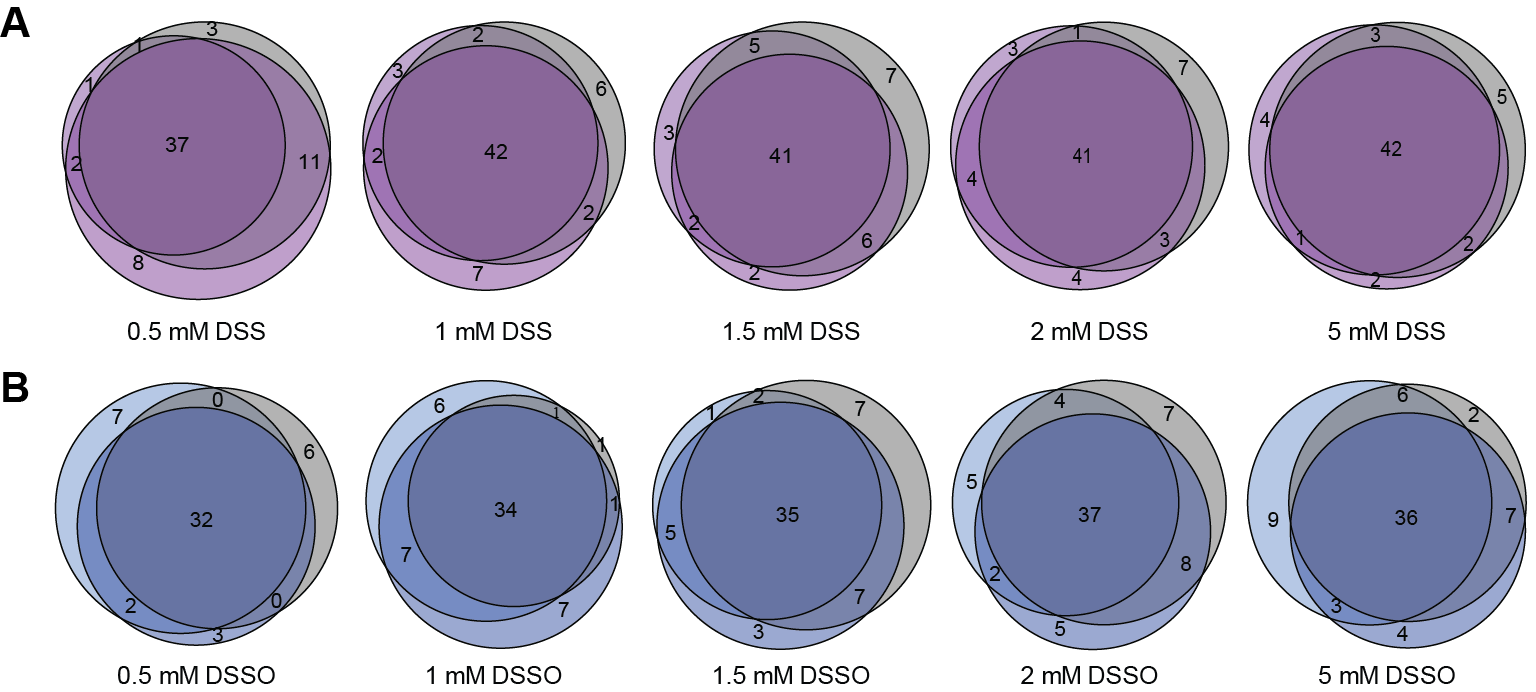
\includegraphics[]{Chapter.2/Figures/SI_Figure2.png} 
        \caption{\textbf{In-gel cross-linking is highly reproducible and only marginally dependent on the concentration of the reagent.} \textbf{A.} Venn diagrams displaying the overlap of detected unique cross-links in triplicate measurements of GroEL cross-linked in gel with different DSS concentrations. \textbf{B.} Venn diagrams displaying the overlap of detected unique cross-links in triplicate measurements of GroEL cross-linked in gel with different DSSO concentrations.}
        \label{fig:ch2_app_fig2}
    \end{figure*}

    \clearpage

    \begin{figure*}[hbt!]
        \center
        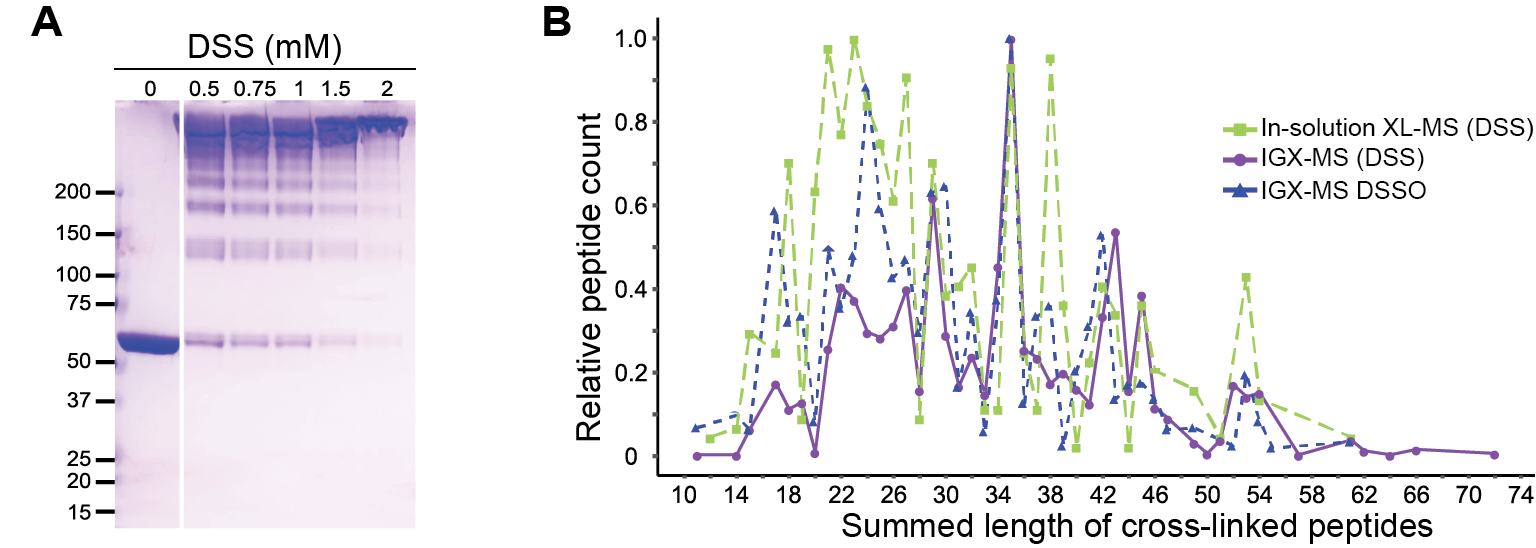
\includegraphics[]{Chapter.2/Figures/SI_Figure3.png} 
        \caption{\textbf{Optimization of cross-linker concentration for in-solution XL-MS and observed cross-linked peptide length distributions for IGX-MS and in-solution XL-MS.} \textbf{A.} GroEL was cross-linked in-solution using different DSS concentrations for the optimization of the cross- linker concentration. The samples were then loaded onto a SDS-PAGE for visualization. A concentration of
        0.75 mM DSS was selected for further experiments. \textbf{B.} Comparison of summed length of cross-linked peptide-pairs from IGX-MS (1.5 mM DSS or 2 mM DSSO) or in-solution XL-MS (0.75 mM DSS) experiments.}
        \label{fig:ch2_app_fig3}
    \end{figure*}

    \begin{figure*}[hbt!]
        \center
        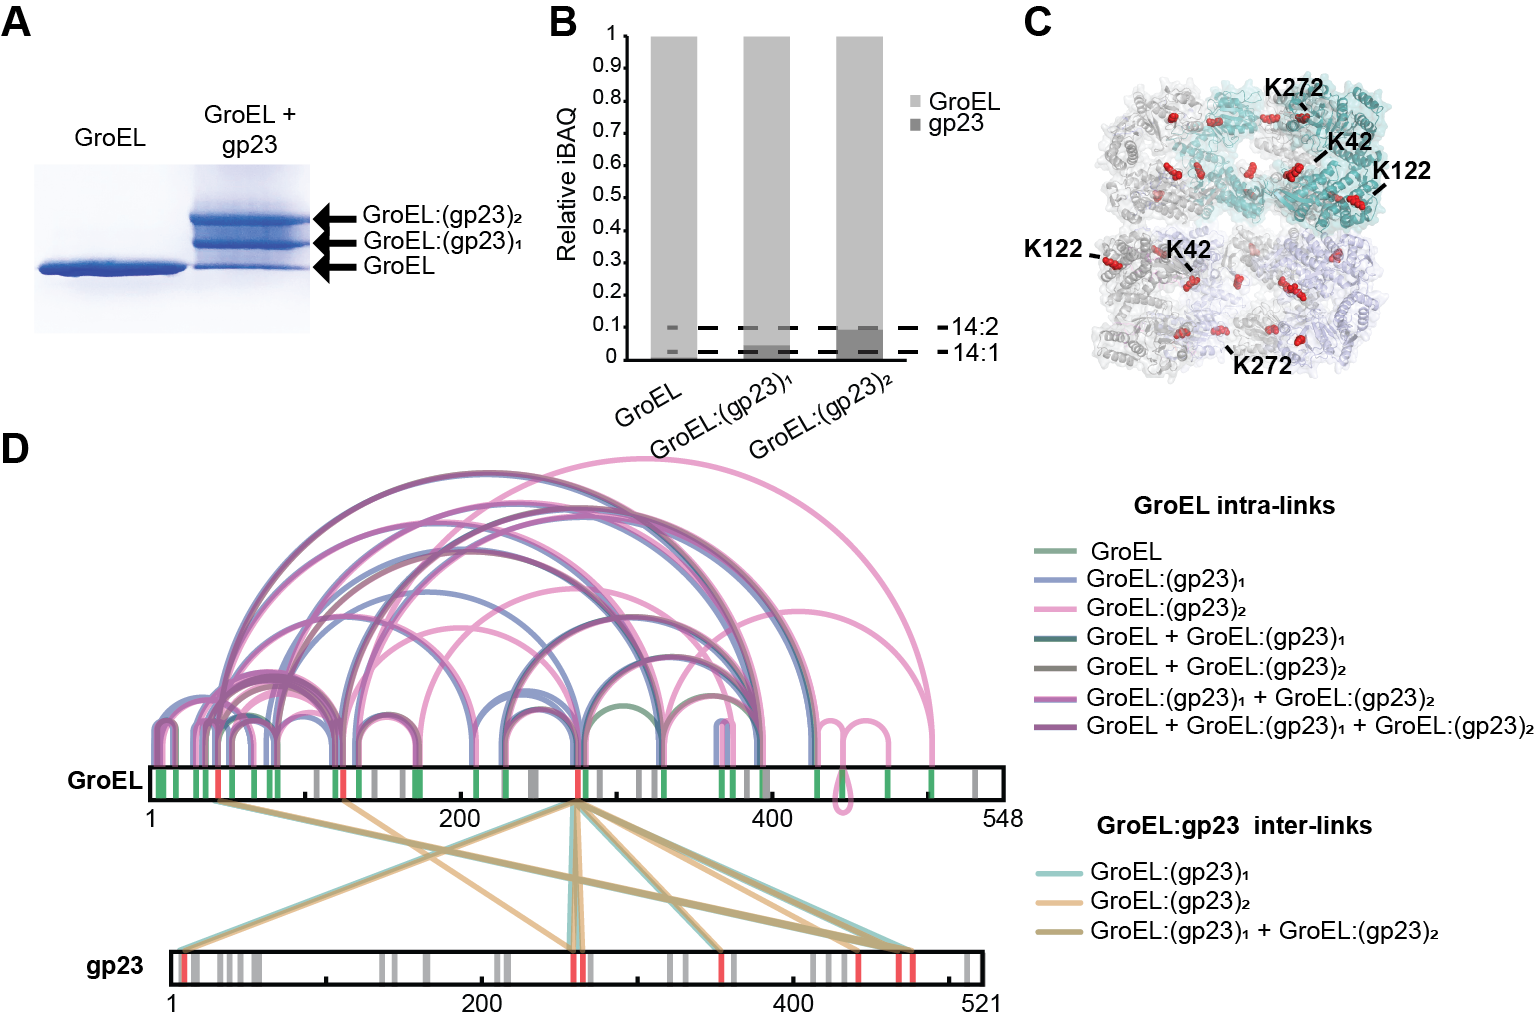
\includegraphics[]{Chapter.2/Figures/SI_Figure4.png} 
        \caption{\textbf{IGX-MS of GroEL bound to the gp23 substrate.} \textbf{A.} BN-PAGE of GroEL incubated with or without unfolded gp23. The arrows indicate free GroEL or GroEL bound to one or two molecules of gp23. \textbf{B.} Label-free quantification for the estimation of the stoichiometry of the formed complexes. Relative iBAQ values of GroEL and gp23 in the three bands. Dashed lines indicate the GroEL:gp23 ratios for the theoretically expected 14:1 and 14:2 ratios. \textbf{C.} Cross-section of the structural model of GroEL (PDB ID: 1KP8) with lysine residues that were found to be cross-linked to gp23 shown in red spheres. \textbf{D.} Overlay of cross-links identified in the three bands, representing the GroEL, the GroEL:gp23, and GroEL:(gp23)2 complex. GroEL intra-links are colored green, purple, and pink. Inter-links are colored turquoise and sand. For clarity, intra-links in gp23 are not depicted. Grey lines in the sequence indicate lysine residues not cross-linked, red lines indicate inter-linked lysine residues, and green lines indicate intra-linked residues.}
        \label{fig:ch2_app_fig4}
    \end{figure*}

    \begin{figure*}[hb!]
        \center
        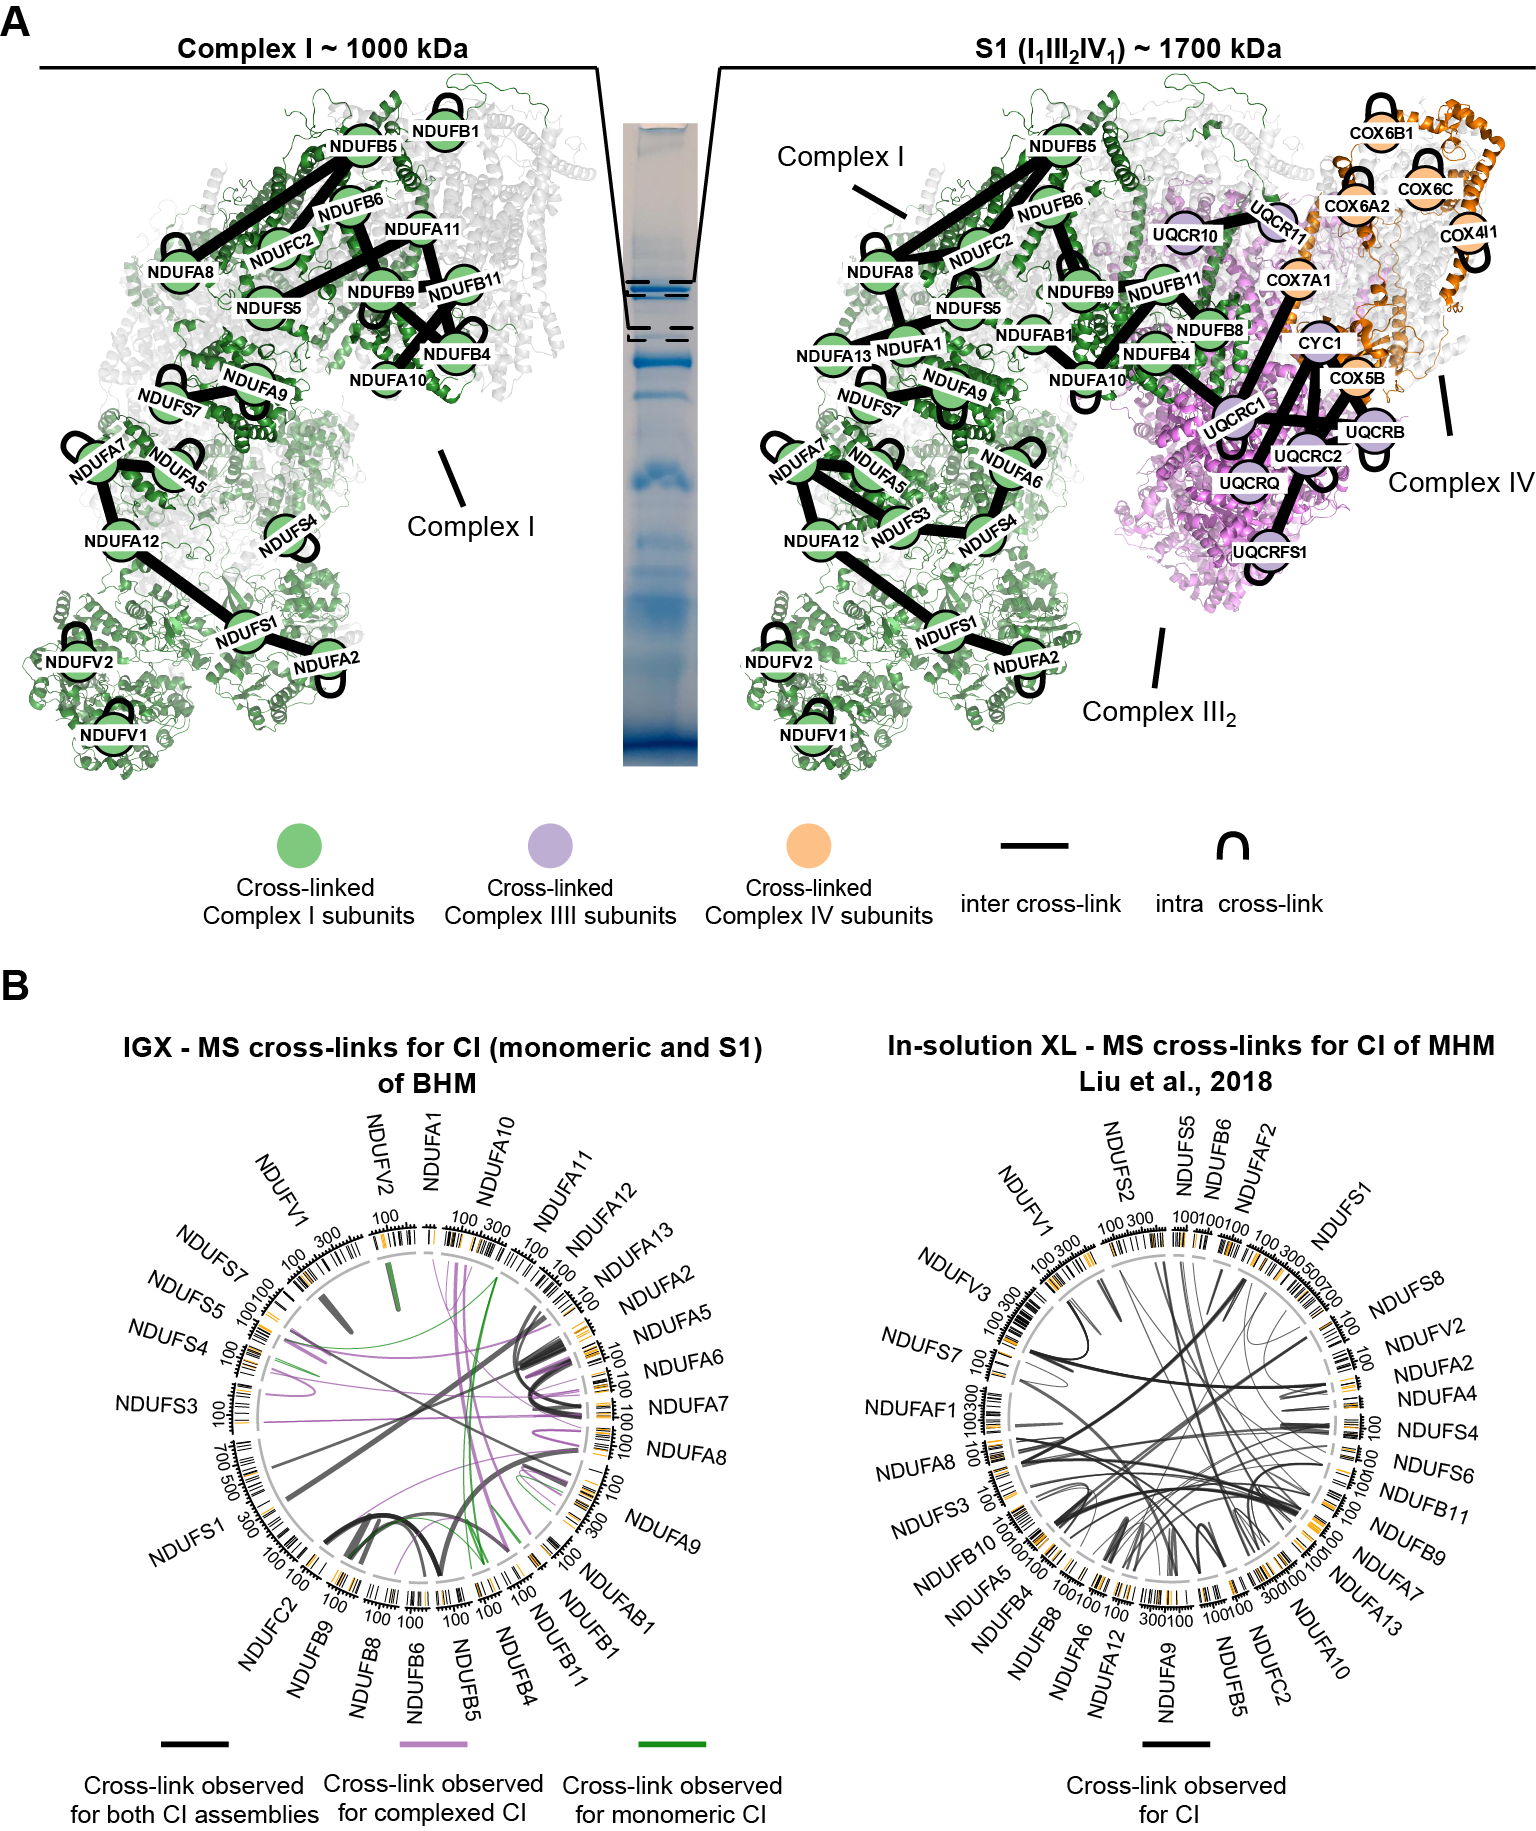
\includegraphics[]{Chapter.2/Figures/EV_Figure1.png} 
        \caption{}
        \label{fig:ch2_app_fig5}
    \end{figure*}

    \addtocounter{figure}{-1}
    \begin{figure*}[ht!]
        \caption{\textbf{Assembly state specific cross-linking of Complex I from bovine heart mitochondria (BHM) in its monomeric state and when incorporated within a super-complex by IGX-MS.} \textbf{A.} IGX-MS cross-links observed within monomeric complex I (left) - and when incorporated within the super complex S1 (right). Node positions are in accordance with respective subunit coordinates of the published S1 structure (PDB ID: 5GUP). \textbf{B.} Circos plots of detected cross-links within the monomeric complex I (CI) (black Gene names) identified by IGX-MS (left panel) and in-solution XL-MS (right panel). The position of the lysine residues is shown in the outer-ring, and cross-linked residues are colored dark orange. For IGX-MS generated data (left panel), cross-links are colored based on the CI assembly state they were detected for. For in-solution XL-MS (right panel) the cross-links originated from a mixture of all assembly states of CI present in-solution. Thickness of the cross-link lines correlates to the number of detected cross-linked spectra matches (CSMs).}
    \end{figure*}

    \begin{figure*}[hbt!]
        \center
        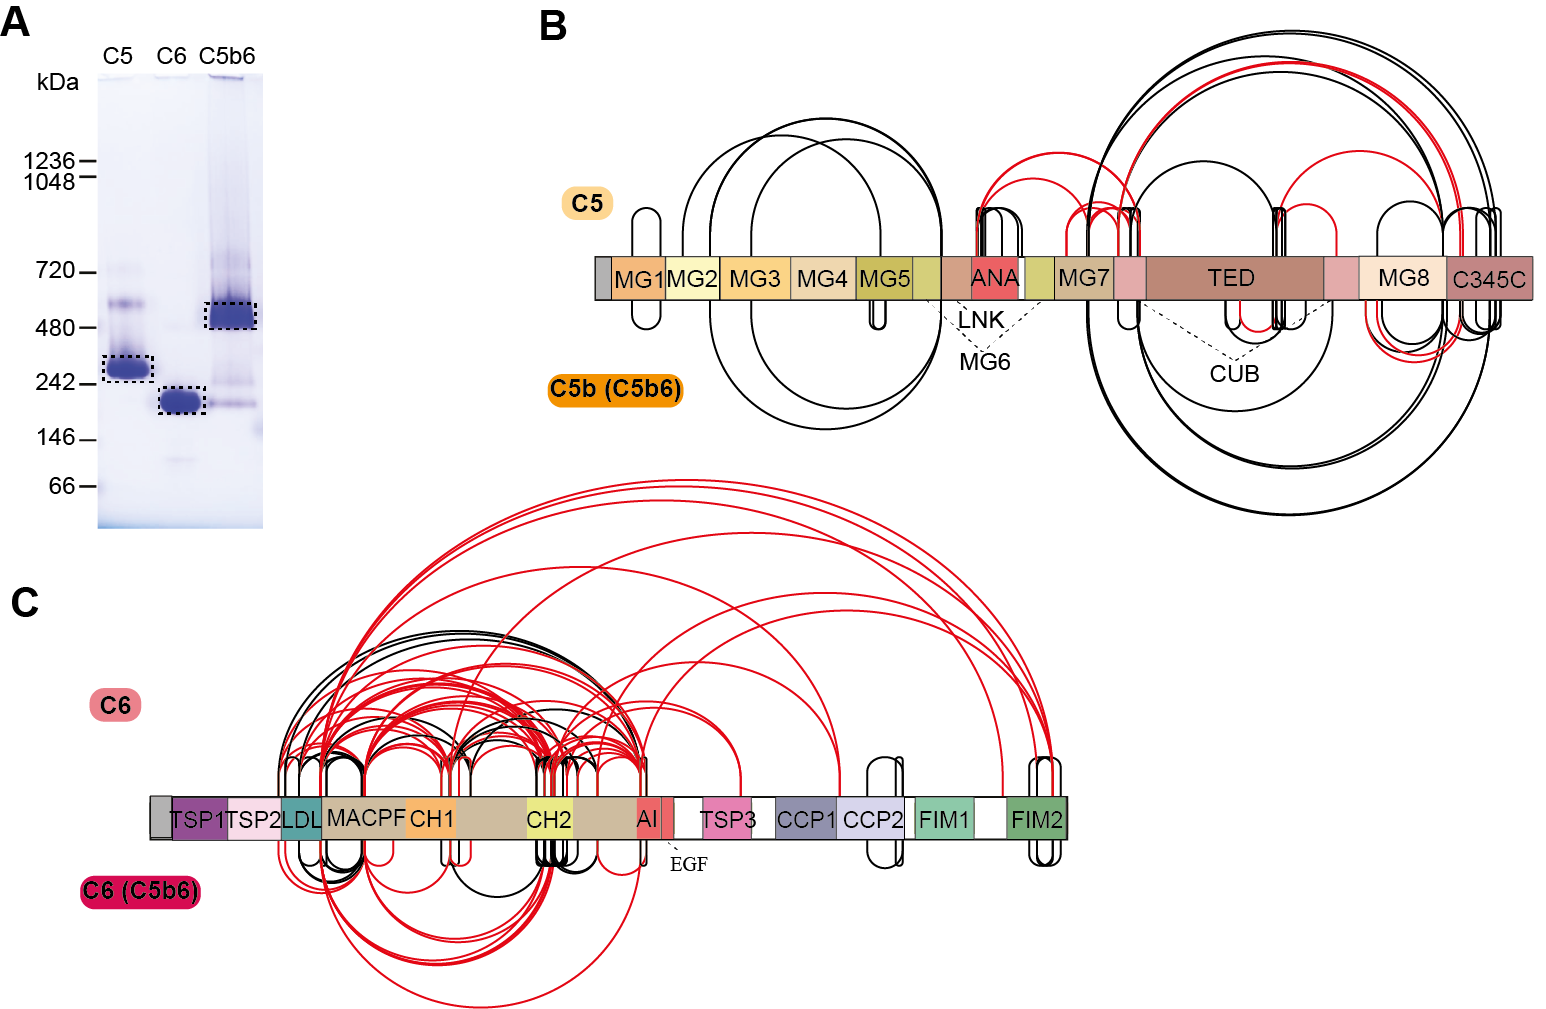
\includegraphics[]{Chapter.2/Figures/SI_Figure5.png} 
        \caption{\textbf{IGX-MS of C5, C6, and C5b6.} \textbf{A.} BN-PAGE of complement components C5, C6, and the C5b6 complex. For each lane 5 $\mu$g of protein (C5, C6), respectively 10 $\mu$g (C5b6) of protein, were applied onto the gel. Dashed boxes indicate the bands cut out for subsequent IGX-MS analysis. \textbf{B-C.} Schematic overview for domain-centered cross-link results for C5 and Cb5b in the C5b6 complex (B) or C6 and C6 in the C5b6 complex (C). Black lines indicate cross-links within the distance restraints ($\leq$ 30 Å). Red lines indicate cross-links exceeding the distance restraints ($\geq$ 30 Å). Notably, for C6, many cross-links to the N-terminal domains are not present when C6 is complexed to C5b.}
        \label{fig:ch2_app_fig6}
    \end{figure*}

    \begin{figure*}[hbt!]
        \center
        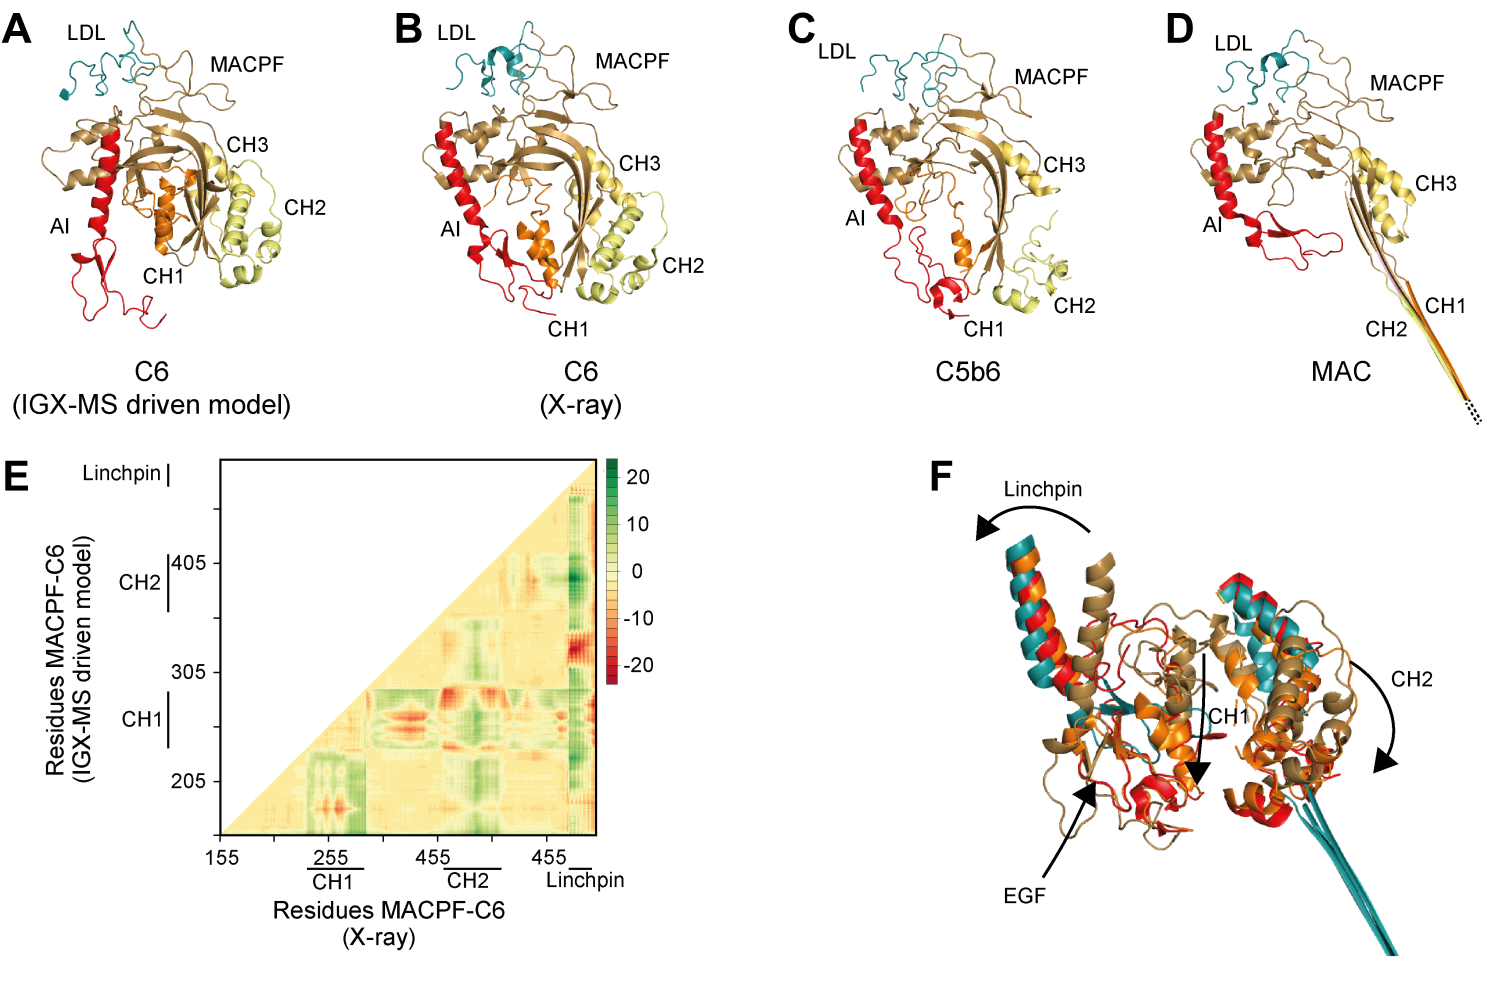
\includegraphics[]{Chapter.2/Figures/EV_Figure2.png} 
        \caption{\textbf{Structural rearrangements of the AI and CH regions of C6 when going from free C6, the C5b6 intermediate structure to C6 in the fully assembled MAC.} \textbf{A-D.} Cartoon representation of the LDL (deepcyan) and MACPF (sand) domains within the IGX-MS driven C6 model (A), C6 from the X-ray structure (PDB ID: 3T5O) (B), C6 complexed with C5b (PDB ID: 4A5W) (C), and C6 as part of the MAC (PDB ID: 6H03) (D). The regions CH 1-3 (orange, paleyellow, and yelloworange) and auto-inhibitory (AI, red) within MACPF are shown. \textbf{E.} The difference distance matrix of superposed C6-MACPF domains. The difference distance was calculated by substracting the coordinates of aligned MACPF backbones of the IGX-MS driven model and the I-tasser model (for complete sequence coverage) of C6 -X-ray structure (PDB ID: 3T5O). The distance values are plotted with colors representing C$\alpha$ differences of -20 to 20 Å according to the right-sided scale. \textbf{F.} Overlay of the AI (composed of linchpin helix and EGF domain), CH1, and CH2 regions of MACPF in four distinct conformations of C6, namely the IGX-MS driven model (sand), the deposited C6 X-ray structure (orange), when incorporated in the C5b6 complex (red), and finally when incorporated in the fully assembled MAC (deepcyan). Arrows indicate the conformational changes of the different regions from free C6 (IGX-MS driven model) to partial activation (PDB ID: 3T5O) and C5b binding (PDB ID: 4A5W) and final assembly into the MAC (PDB ID: 6H03).}
        \label{fig:ch2_app_fig7}
    \end{figure*}

    \begin{figure*}[hbt!]
        \center
        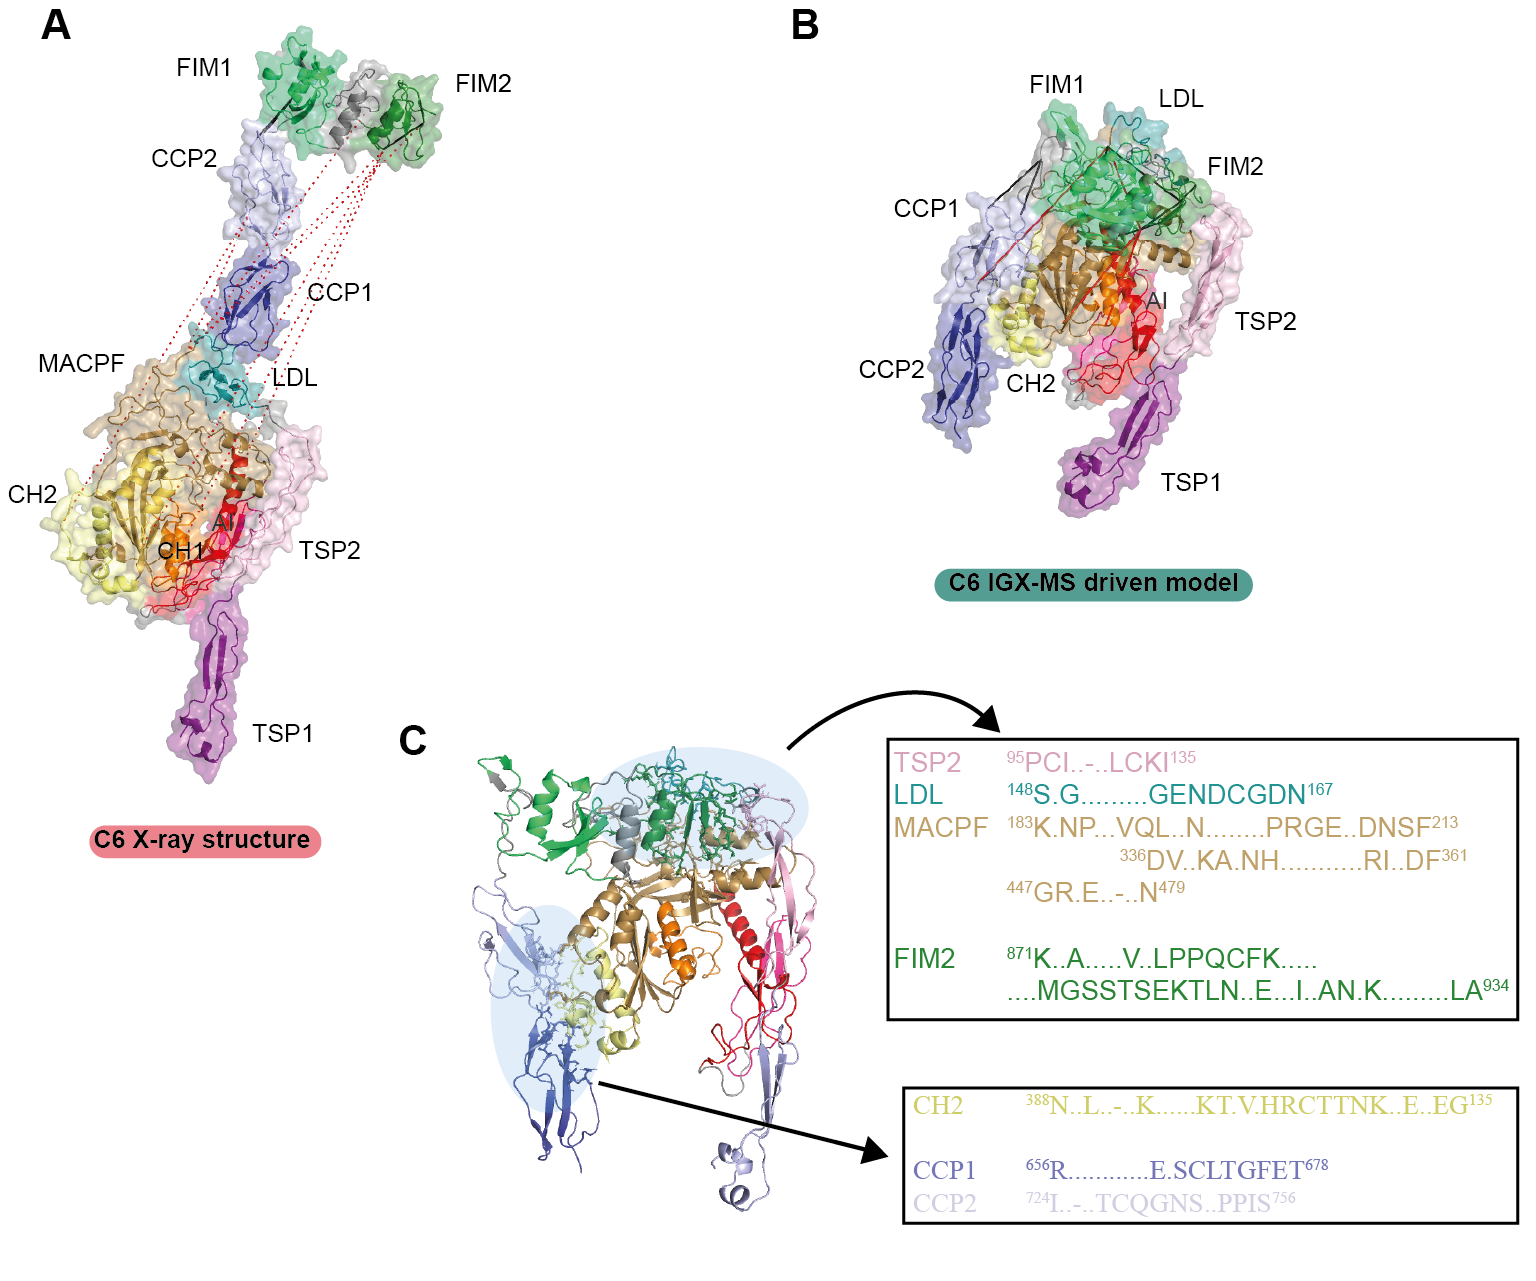
\includegraphics[]{Chapter.2/Figures/SI_Figure6.png} 
        \caption{\textbf{Comparison of the monomeric C6 X-ray structure and IGX-MS driven structural model, wherein the C5b-binding region becomes docked to the main body.} \textbf{A.} Cross-links identified for residues in the C5b-binding region plotted onto the C6 X-ray structure (PDB ID: 3T5O). Cross-links that were used to dock the C5b-binding domain (CCP1-2, FIM1-2) to the LDL- and MACPF domain are shown as dotted lines. Black lines indicate cross-links within the distance restraints ($\leq$ 30 Å). Red lines indicate cross-links exceeding the distance restraints ($\geq$30 Å). \textbf{B.} IGX-MS driven structural model of free C6. Cross-links obtained for the C5b-binding region are plotted onto the final model of C6. Solid black lines indicate distances below 30 Å, and red dotted lines indicate links with a distance larger than 30 Å. \textbf{C.} Interaction interface analysis for C5b-binding and the LDL-, MACPF domains. Blue circles indicate binding interfaces, for which interacting residues were identified (shown as sticks). The identified interacting residues of the different domains are shown in the black boxes.}
        \label{fig:ch2_app_fig8}
    \end{figure*}

    \begin{figure*}[hbt!]
        \center
        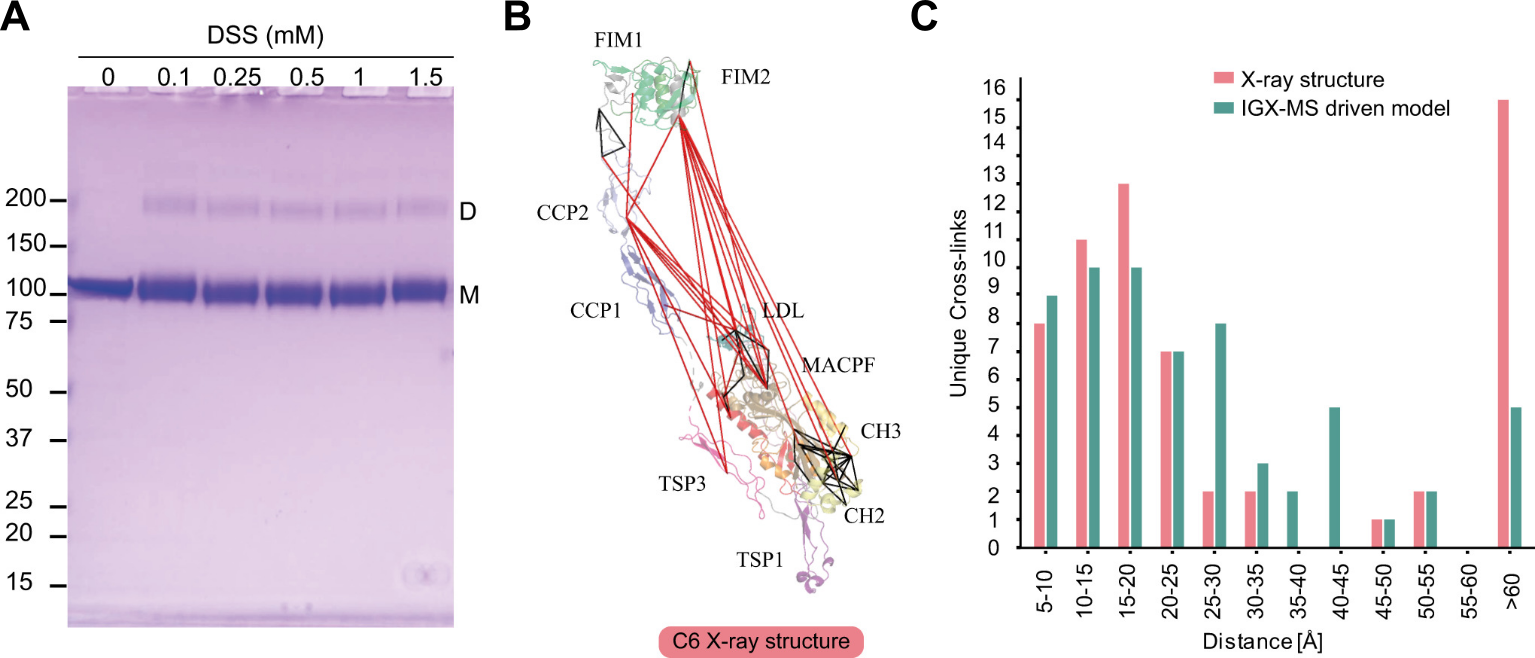
\includegraphics[]{Chapter.2/Figures/EV_Figure3.png} 
        \caption{\textbf{In-solution XL-MS of C6.} \textbf{A.} DSS concentration optimization for cross-linking C6 in-solution monitored by SDS-PAGE. The upper band ($\sim$200 kDa) indicates a C6 dimer that is formed upon cross-linking whereas the more abundant lower band ($\sim$100 kDa) represents monomeric C6. \textbf{B.} Obtained cross-links for monomeric C6 plotted on the available X-ray structure of C6 (PDB ID: 3T5O). The red lines indicate distances > 30 Å. The different domains of C6 are indicated in black. \textbf{C.} Distribution of lysine C$\alpha$-C$\alpha$ distances of unique cross-links identified by in-solution XL-MS for monomeric C6 when plotted on the reported X-ray structure (pink bars, PDB ID: 3T5O) and the IGX-MS driven refined structural model (green bars). The average distance of all cross-links is 41.7 Å when using the X-ray structure which reduces to 26.2 Å for the IGX-MS driven structural model.}
        \label{fig:ch2_app_fig9}
    \end{figure*}

    \begin{figure*}[hbt!]
        \center
        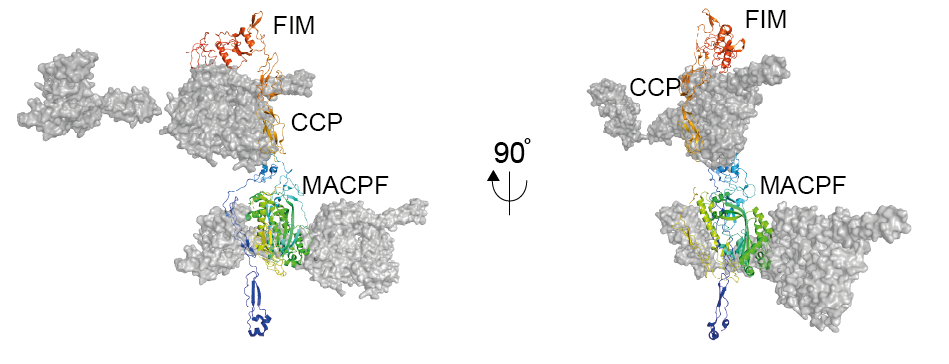
\includegraphics[]{Chapter.2/Figures/SI_Figure7.png} 
        \caption{\textbf{Possible interactions between adjacent C6 molecules in the deposited X-ray crystal structure.} The total electron density acquired for the X-ray structure of C6 (PDB ID: 3T5O) reveals closely packed neighboring C6 molecules. A single C6 molecule is shown here in a rainbow-colored cartoon in two orientations. The surface (grey) of two adjacent C6 molecules in the electron density maps shows the interaction of the C-terminal CCP and FIM domains of one C6 molecule with the MACPF domain of another C6 molecule.}
        \label{fig:ch2_app_fig10}
    \end{figure*}

\end{subappendices}

\clearpage
\section*{References}
\bibliographystyle{Style_settings/bibstyle_pnas}
\bibliography{Chapter.2/chapter2_bib_form}

\end{document}